% My Bachelor's thesis

\documentclass[
11pt, % The default document font size, options: 10pt, 11pt, 12pt
%oneside, % Two side (alternating margins) for binding by default, uncomment to switch to one side
english, % ngerman for German
singlespacing, % Single line spacing, alternatives: onehalfspacing or doublespacing
%draft, % Uncomment to enable draft mode (no pictures, no links, overfull hboxes indicated)
%nolistspacing, % If the document is onehalfspacing or doublespacing, uncomment this to set spacing in lists to single
%liststotoc, % Uncomment to add the list of figures/tables/etc to the table of contents
%toctotoc, % Uncomment to add the main table of contents to the table of contents
%parskip, % Uncomment to add space between paragraphs
%nohyperref, % Uncomment to not load the hyperref package
headsepline, % Uncomment to get a line under the header
%chapterinoneline, % Uncomment to place the chapter title next to the number on one line
%consistentlayout, % Uncomment to change the layout of the declaration, abstract and acknowledgements pages to match the default layout
]{MastersDoctoralThesis} % The class file specifying the document structure

\usepackage[utf8]{inputenc} % Required for inputting international characters
\usepackage[T1]{fontenc} % Output font encoding for international characters
\usepackage{algorithm}
\usepackage{minted}
\usepackage{xcolor}
\usepackage{gentium}
\usepackage{graphicx}
\usepackage{pdfpages}
\usepackage{caption}
\usepackage{subcaption}
\usepackage{grffile}
\usepackage{longtable}
\usepackage{wrapfig}
\usepackage{rotating}
\usepackage[normalem]{ulem}
\usepackage{amsmath}
\usepackage{textcomp}
\usepackage{tabularx}
\usepackage{booktabs}
\usepackage{amssymb}
\usepackage{capt-of}
\usepackage{hyperref}
\usepackage{float}
%\usepackage[compact]{titlesec}
%\usepackage{mathpazo} % Use the Palatino font by default
\usepackage[backend=biber]{biblatex} % Use the bibtex backend with the authoryear citation style (which resembles APA)

\addbibresource{bibliography.bib} % The filename of the bibliography

\usepackage[autostyle=true]{csquotes} % Required to generate language-dependent quotes in the bibliography

%----------------------------------------------------------------------------------------
%	MARGIN SETTINGS
%----------------------------------------------------------------------------------------

\geometry{
	paper=a4paper, % Change to letterpaper for US letter
	inner=2.5cm, % Inner margin
	outer=3.8cm, % Outer margin
	bindingoffset=.5cm, % Binding offset
	top=1.5cm, % Top margin
	bottom=1.5cm, % Bottom margin
	%showframe, % Uncomment to show how the type block is set on the page
}

%----------------------------------------------------------------------------------------
%	THESIS INFORMATION
%----------------------------------------------------------------------------------------

\thesistitle{Machine Learning techniques in the searches for resonant signatures at the LHC} % Your thesis title, this is used in the title and abstract, print it elsewhere with \ttitle
\supervisor{Dr. Halil Saka} % Your supervisor's name, this is used in the title page, print it elsewhere with \supname
%\examiner{} % Your examiner's name, this is not currently used anywhere in the template, print it elsewhere with \examname
\degree{Physics} % Your degree name, this is used in the title page and abstract, print it elsewhere with \degreename
\author{Konstantinos Papadimos} % Your name, this is used in the title page and abstract, print it elsewhere with \authorname
\addresses{} % Your address, this is not currently used anywhere in the template, print it elsewhere with \addressname

\subject{Particle Physics} % Your subject area, this is not currently used anywhere in the template, print it elsewhere with \subjectname
\keywords{} % Keywords for your thesis, this is not currently used anywhere in the template, print it elsewhere with \keywordnames
\university{University of Cyprus} % Your university's name and URL, this is used in the title page and abstract, print it elsewhere with \univname
\department{Department of Physics} % Your department's name and URL, this is used in the title page and abstract, print it elsewhere with \deptname
%\group{\href{http://researchgroup.university.com}{Research Group Name}} % Your research group's name and URL, this is used in the title page, print it elsewhere with \groupname
\faculty{Faculty of Pure and Applyed Sciences} % Your faculty's name and URL, this is used in the title page and abstract, print it elsewhere with \facname

\AtBeginDocument{
\hypersetup{pdftitle=\ttitle} % Set the PDF's title to your title
\hypersetup{pdfauthor=\authorname} % Set the PDF's author to your name
\hypersetup{pdfkeywords=\keywordnames} % Set the PDF's keywords to your keywords
}

\begin{document}

\frontmatter % Use roman page numbering style (i, ii, iii, iv...) for the pre-content pages

\pagestyle{plain} % Default to the plain heading style until the thesis style is called for the body content

%----------------------------------------------------------------------------------------
%	TITLE PAGE
%----------------------------------------------------------------------------------------

\begin{titlepage}
\begin{center}

\vspace*{.06\textheight}
{\scshape\LARGE \univname\par}\vspace{1.5cm} % University name
\textsc{\Large Bachelor Thesis}\\[0.5cm] % Thesis type

\HRule \\[0.4cm] % Horizontal line
{\huge \bfseries \ttitle\par}\vspace{0.4cm} % Thesis title
\HRule \\[1.5cm] % Horizontal line
 
\begin{minipage}[t]{0.4\textwidth}
\begin{flushleft} \large
\emph{Author:}\\
\href{http://www.johnsmith.com}{\authorname} % Author name - remove the \href bracket to remove the link
\end{flushleft}
\end{minipage}
\begin{minipage}[t]{0.4\textwidth}
\begin{flushright} \large
\emph{Supervisor:} \\
\href{http://www.jamessmith.com}{\supname} % Supervisor name - remove the \href bracket to remove the link  
\end{flushright}
\end{minipage}\\[3cm]
 
\vfill

\large \textit{A thesis submitted in fulfillment of the requirements\\ for the degree of \degreename}\\[0.3cm] % University requirement text
\textit{in the}\\[0.4cm]
\facname\\\deptname\\[2cm] % Research group name and department name
 
\vfill

{\large \today}\\[4cm] % Date
%\includegraphics{Logo} % University/department logo - uncomment to place it
 
\vfill
\end{center}
\end{titlepage}

%----------------------------------------------------------------------------------------
%	ABSTRACT PAGE
%----------------------------------------------------------------------------------------

\begin{abstract}
This work presents a study of the interplay between multivariate and single variate classification techniques, and energy scale uncertainties in the search for heavy and light diobject resonances at the LHC. The performance of a Boosted Decision Tree (BDT) model and a fit-based analysis is explored under various cases of energy scale uncertainties.

The study concludes that a multivariate classification method, like the BDT model, is better suited when systematic uncertainties are introduced to the problem, as univariate classification techniques can be challenging in such cases.\ldots
\end{abstract}

%----------------------------------------------------------------------------------------
%	LIST OF CONTENTS/FIGURES/TABLES PAGES
%----------------------------------------------------------------------------------------

\tableofcontents % Prints the main table of contents

%\listoffigures % Prints the list of figures

%\listoftables % Prints the list of tables

%----------------------------------------------------------------------------------------
%	THESIS CONTENT - CHAPTERS
%----------------------------------------------------------------------------------------

\mainmatter % Begin numeric (1,2,3...) page numbering

\pagestyle{thesis} % Return the page headers back to the "thesis" style

% Include the chapters of the thesis as separate files from the Chapters folder
% Uncomment the lines as you write the chapters

\section{Theoritical Overview}
\label{sec:org2ae82f1}
\subsection{Units in particle physics}
\label{sec:org2338bc0}
Particle physics, study the properites of subatomic particles and their interactions. To describe such microscopic phenomena and quantities, an appropriate system of units must be adopted, for if the SI system of units was to be used, one would have to deal with large exponents. More over, it is more practical to utilize a system that is based on the typical length and time scales found in particle physics[modern particle phyics].

The foundamental constants of the special theory of relativity, as well as quantum mechanics are \(\hbar\), c, and  GeV and they can be used as a basis to form a system of units, the Natural Units. Natural units can be further simplified by chosing:
\[ c = \hbar = 1\]
The table below sumarizes the relationship between natural units and S.I

\begin{table}[h!]
\centering
\begin{tabular}{ |p{3cm}|p{4cm}|p{3cm}|  }
 \hline
 \multicolumn{3}{|c|}{Relationship between natural units and S.I} \\
 \hline
 \hline
Quanity & Natural units($ \hbar = c = 1 $) & S.I \\
 \hline
Energy & GeV & $Kg m^{2}s^{-2}$ \\
Momentum & GeV& $ Kg m^{2}s^{-2}$ \\
Mass & GeV & Kg\\
Time & $GeV^{-1}$ & s\\
Length & $GeV^{-1}$ & m\\
 \hline
\end{tabular}
\caption{Some basic quantites in S.I and in Natural units .}
\label{table:natural_units}
\end{table}

\subsection{Special Relativity}
\label{sec:orgd8ae263}

\subsubsection{Four-Vectors - Lorentz transformations}
\label{sec:orgec107fd}

Let S and S' be two inertial reference systems, with S' moving at (a relativistic) 2velocity \(u\) relative to S. The coordinates are chosen such that the motion is along the x-axis in both reference systems. The clocks of both S and S' are synchronized so that when \(x = x' = 0\), \(t = t' = 0\).
For an event with coordinates (x, y, z, t) in S, the coordinates in S' are given by the Lorentz transformations:

\begin{equation}
\begin{matrix}
(x')^{0} = \gamma(x^{0} - \beta x^{1}) \\
(x')^{1} = \gamma(x^{1} - \beta x^{0}) \\
(x')^{2} = x^{2} \\
(x')^{3} = x^{3}
\end{matrix}
\end{equation}
where \(\beta \equiv \frac{u}{c}\text{,   } x^{0}\equiv ct\text{,    } x^{1}\equiv x\text{,   } x^{2}\equiv y\text{,   } x^{3}\equiv z\)

The elements \(x^{i}\text{, i = 0, 1, 2, 3}\) define the position four vector. Mathematicaly four vectors are 4 dimentional, rank 1 tensors that transform according to lorentz transformations

With the introduction of four vectors, using Einstein's summation convention, lorentz transformations can be written as:
\begin{equation}
(x')^{i} = \Lambda^{i}_{j}x^{j}
\end{equation}
Where \(\Lambda\), is the Lorentz transformation matrix, a rank 2 tensor:

\begin{equation}
\Lambda = \begin{pmatrix}
 \gamma & -\gamma \beta &  0 & 0 \\
  -\gamma \beta & \gamma &   0 & 0 \\
  0 & 0& 1 &0\\
  0 & 0& 0 &1\\
  \end{pmatrix}
  \end{equation}

The following quantity does not change under lorentz transformation:
\begin{equation}
I^{2} = -(x^{0})^{2} + (x^{1})^{2} + (x^{2})^{2} +(x^{3})^{2} = -(x'^{0})^{2} + (x'^{1})^{2} + (x'^{2})^{2} +(x'^{3})^{2}
\end{equation}
or written in a more compact form:
\begin{equation}
I = g_{\mu \nu}x^{\mu}x^{\nu} = x^{\mu}x_{\mu}
\end{equation} 
where \(g_{\mu\nu}\) is the Minkowski (metric) tensor:

\begin{equation}
g_{\mu \nu} = \begin{pmatrix}
-1 & 0 & 0 & 0\\
0 & 1 & 0 & 0\\
1 & 0 & 1 & 0\\
1 & 0 & 0 & 1\\
\end{pmatrix}
\end{equation}
Such a quantity as I is called \textbf{invariant}

The introduction of four vectors and the metric tensor, yield the Minkowski Space Time where points need 4 coordinates to be fully described(1, time like and 3 space like ) and the distance between them is beeing defined by the Minkowski tensor. The necessity of four vectors, in order to describe non scalar quantities(such as velocity and momentum) in minkowski space time, is therefore evident.

\subsubsection{Energy and Momentum}
\label{sec:org15fe0da}

According to the principle of relativity, the laws of physics must be the same in all inertial reference systems. Hence, if momentum is conserved  in one inertial frame of reference, it must also be conserved in all others. It is evident that the momentum of a moving particle must be defined in an appropriate manner, to satisfy the principle of relativity \cite{gParticles}. The four momentum is therefore defined as:
\begin{equation}
p^{\mu} = m\eta^{\mu}
\end{equation}
Where \(\eta^{\mu} = \frac{dx^{\mu}}{dt'}\), the four velocity of the particle.

The timelike component of four momentum, expresssed in natural units  is \(p^{0} = \gamma m\). The 3 space like components, constitue the vector momentum, \(\vec{p} = \gamma m\vec{\beta}\).
The relativistic energy is defined as:
\begin{equation}
E = \gamma m = p^{0}
\end{equation}
Thus, the components of four momentum are:
\begin{equation}
p^{\mu} = (E, \vec{p})
\end{equation}

At this point we are able to calculate the invariant "interval" \(p^{\mu}p_{\mu}\) :
\begin{equation}
p^{\mu}p_{\mu} = E^{2} - |\vec{p}|^{2} = m^{2}
\end{equation}
What is invariant in the case of momentum four vector, is the particle's mass. This quantity is called \textbf{invariant mass} of a particle as all observers, in different frames of references, agree upon its value. It is the invariant mass of particles that we can(or we try to) measure, in CERN as well. 

\subsection{The standard model}
\label{sec:org8632faf}

The Standard Model (SM)of particle physics is a theoretical framework that describes the fundamental particles and their interactions through the strong, electromagnetic, and weak forces. Each force is described by a corresponding quantum field theory(QFT). Namely, electromagnetic and weak interactions are described by the electroweak theory and the strong interactions by quantum chromodynamics(QCD). The interactions between particles in each QFT, are described in terms of the exchange of a spin-1 gauge boson. The photon, is the gauge boson of QED, while the gluon, which like the photon has no mass, is the force-carrying particle in the strong interaction. The charged \(W^{+} \text{and }W^{-}\) bosons mediate the weak charged current interaction, which is responsible for \(\beta\) decay and fusion, while the weak neutral current interaction, is mediated by the electrically neutral Z boson. These interactions are also governed by the principles of symmetry and conservation, which dictate that certain properties, such as charge and energy, are conserved during particle interactions

The fundamental particles that comprise all matter according to SM are the already mentioned gauge bosons, quarks, and leptons. The quarks and leptons are organized into three generations, with each generation containing two types of leptons and two types of quarks. The leptons are either negatively charged, with a charge of -1, or electrically neutral. The quarks, on the other hand, have fractional charges of either -1/3 or +2/3, and are characterized by their color, which can be blue, green, or red. Additionally, for each elementary fermion, there is a corresponding antifermion with the same mass and spin but with an opposite electric charge.

Completing the picture of fundamental particles is the scalar boson, the Higgs boson, responsible for giving mass to the other particles. A brief summary of the fundamental particles is presented in Figure \ref{fig:particles}.

\begin{figure}[h]
\centering
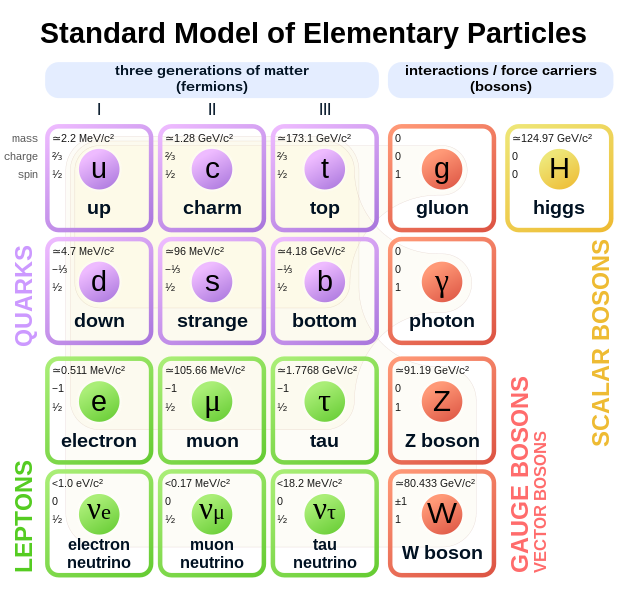
\includegraphics[width=0.35 \textwidth, ext=.png type=png]{/home/kpapad/UG_thesis/Thesis/Dissertation/src/figures/627px-Standard_Model_of_Elementary_Particles.svg.png}
\caption{Summary of the elementary particles. All matter around us is made up by 12 fermions!}
\label{fig:particles}
\end{figure}


The SM has undergone extensive testing through high-energy experiments at CERN, with its predictions confirmed with a high degree of precision. However, the model has limitations, such as its inability to account for dark matter or the observed imbalance between matter and antimatter in the universe.

Despite its limitations, the Standard Model remains a cornerstone of modern physics, and its continued study and refinement is essential to advancing our understanding of the universe at its most fundamental level.
\subsection{Collisions and resonances}
\label{sec:org874321a}
\subsection{Maybe some elements of the theory behind our monte carlo simulations}
\label{sec:orgfe09146}


\section{Accelerators and Detectors: the LHC and the CMS}
\label{sec:org3878a16}
\subsection{The Large Hadron Collider}
\label{sec:org5906b28}
Our knowledge in the field of high energy physics has been largely obtained through fixed target experiments that used proton and electron accelerators. However, over the last decades, the significance of colliding beam experiments has been rising. Such experiments involve two particle beams that rotate in opposite directions and collide at multiple points around the ring. The key advantage of colliding beam machines is their ability to produce new particles due to the high center of mass energy created during the collision. This energy increases linearly as E, rather than as \(E^{1/2}\), in fixed target experiments, and almost all of it is utilized in generating new particles[modern particle physics].

One great example of a colliding beam machine is The Large Hadron Collider (LHC).  The LHC has been instrumental in many groundbreaking discoveries, with the most famous one beeing the Higgs boson, and has helped scientists to further our understanding of the fundamental nature of the universe. The LHC encompasses a 27-kilometre ring consisting of superconducting magnets with numerous accelerating structures along its length.

Within the accelerator, a strong magnetic field is accelerating the two counterrotating proton beams to velocities near that of the speed of light uppon collision.  The thousands of  superconducting magnets, responsible of the generation of the magnetic field, are of varying sizes and types. Dipole magnets, 1232 in total and 15 meters in length, are utilized to bend the beams and quadrupole magnets, 392 in total and 5-7 meters long, focus the beams. Prior to collision, another type of magnet is used to compress the particles, increasing the likelihood of collisions \href{https://www.lhc-closer.es/taking\_a\_closer\_look\_at\_lhc/0.momentum}{source}.
\subsection{The Compact Muon Solenoid}
\label{sec:orgccfbfe1}
The main goal of  the Compact Muon Solenoid (CMS), as a general purpose particle detector, is to  to reconstruct the Feynman diagram associated with any interaction that might happen inside the LHC. The first and foremost interactions that happen are the collisions between the beams, which generate individual interactions known as \emph{events}. Even though most of the particles associated with an event are unstable, their final decay products, are stable enough to reach the detector and be measured. In the rest of the chapter I will give a brief overview of the CMS detector and discus how does it detect particles.
\subsubsection{Overview}
\label{sec:org3cfeb42}
The CMS detector consists of 5 compartments, each with unique functionality, that are organised in several coaxial layers. The Silicon Tracker, located in the innermost part of CMS, includes silicon pixel vertex detectors and silicon strip detectors, which trace the position and momentum of charged particles. The Electromagnetic Calorimeter (ECAL), the second layer, is composed of PbWO4 crystals and intended to detect photons and electrons. The Hadronic Calorimeter (HCAL), the third layer, is designed to identify hadrons. The Superconducting Solenoid Magnet, the fourth layer, is an solenoid coil that generates a constant magnetic field of 4 T along the direction of the  beam. Due to the deflection of the trajectories of charged particles by the magnet, it becomes possible to measure their momentum. The final, outer most layer, is responsible for the measurement of muon the tracks. Figure \ref{fig:CMS_detector} provides a sectional view of the CMS detector[\url{https://cms.cern/news/cms-detector-design}].
\begin{figure}[hb]
\centering
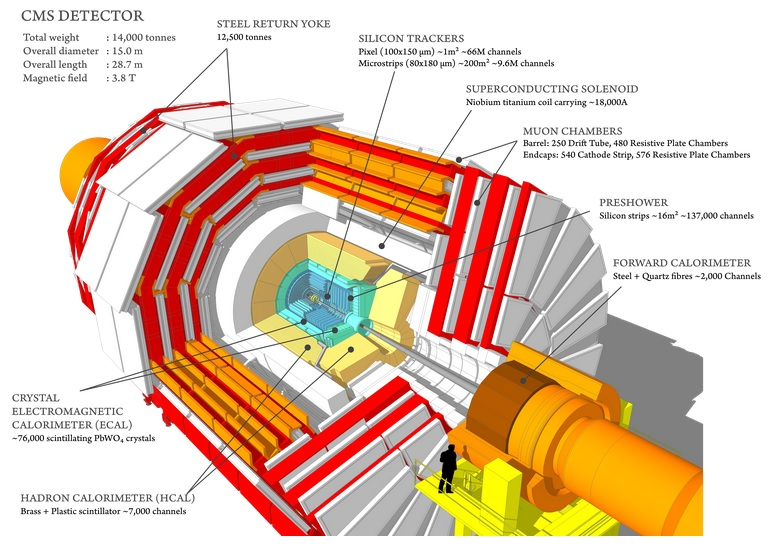
\includegraphics[width=0.8 \textwidth, ext=.png type=jpg]{/home/kpapad/UG_thesis/Thesis/Dissertation/src/figures/cms_detector.jpg}
\caption{A cross-sectional perspective of the CMS detector}
\label{fig:CMS_detector}
\end{figure}

\subsubsection{Coordinate convention at the CMS}
\label{sec:orge8fa37a}
Given the solenoid geometry of the CMS detector, it is more convenient to use a spherical type of coordinates\(\left(r, \phi, \theta \right)\). The origin is located at the collision point and the z axis is parallel to the beam as shown in figure \ref{fig:CMSCoords}. In this system, the momentum of a particle(or any other vector) can be analyzed in a component parallel to the z axis and one component perpendicular to the z axis(Transverse mometnum). Transverse mometnum is defined as follows:
\begin{equation}
|\vec{P_{T}}| = \sqrt{P_{x}^{2} + P_{y}^{2}} = |\vec{P}|\sin{\phi}
\end{equation}
Where \(|\vec{P}| = \sqrt{P_{x}^{2} + P_{y}^{2} + P_{z}^{2}}\). The CMS detector, measures the transverse energy(\href{https://www.lhc-closer.es/taking\_a\_closer\_look\_at\_lhc/0.momentum}{source} ) of particles, and thus it is useful to work with the transverse momentum \(P_{T}\). The azimuth angle  \(\phi \in \left[0, 2\pi\right)\) coordinate is the angle between \(P_{t}\) and x axis and the polar angle  \(\theta \in \left[0, \pi   \right]\) is the angle between the momentum vector and the z axis.

\begin{figure}[ht]
\centering
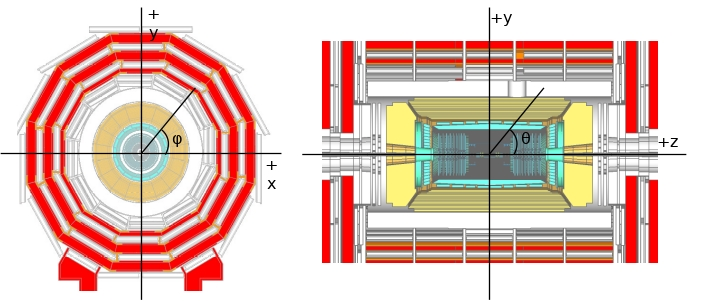
\includegraphics[width=0.7 \textwidth, ext=.png type=jpg]{/home/kpapad/UG_thesis/Thesis/Dissertation/src/figures/cms_coords.jpg}
\caption{CMS coordinates}
\label{fig:CMSCoords}
\end{figure}


Due to the relativistic nature of the phenomena taking place inside LHC, it is more usefull to work with lorentz invariant quantities [V. Chiochia (2010) Accelerators and Particle Detectors from University of Zurich]. Thus, instead of working with the polar angle it is more convenient to introduce the lorentz invariant  \emph{pseudorapidity} \(\eta\in \left [ -\infty, +\infty \right ]\).  Pseudorapidity is defined as:
\begin{equation}
\eta \equiv -\ln{\left [ \tan\left (\frac{\theta}{2} \right ) \right]  }
\end{equation}

The cartesian\(p_{x}\text{, } p_{y}\text{, }p_{z}\) momentum components are related to the \(P_{T}\text{, }\eta\text{, }\phi\)  components by the following transformation relations:
\begin{equation}
\begin{matrix}
p_{x} = P_{T}\cos{\phi} \\
p_{y} = P_{T}\sin{\phi} \\
p_{z} = P_{T}\sinh{\eta}\\
|\vec{P}| = P_{T}\cosh{\eta} 
\end{matrix}
\end{equation}

\subsubsection{Position tracking and momentum measurements: Silicon Tracker}
\label{sec:org2c477d8}
The Silicon tracker measures the positions of charged particles at a number of points, thus it is able to record their trajectory. Given the radius of curvature of the particle's track(due to the 4T magnetic field of the super conducting solenoid), the tracker provides sufficient information, to reconstruct the momentum of the particle. More over, the geometrical location of the trajectory gives direct information regarding the position of the particle. Therefore, the silicon tracker measurements  provide  information regarding the \(P_{T}\text{, } \eta\text{ and }\phi\) of the particles that it detects.

\begin{figure}[ht]
\centering
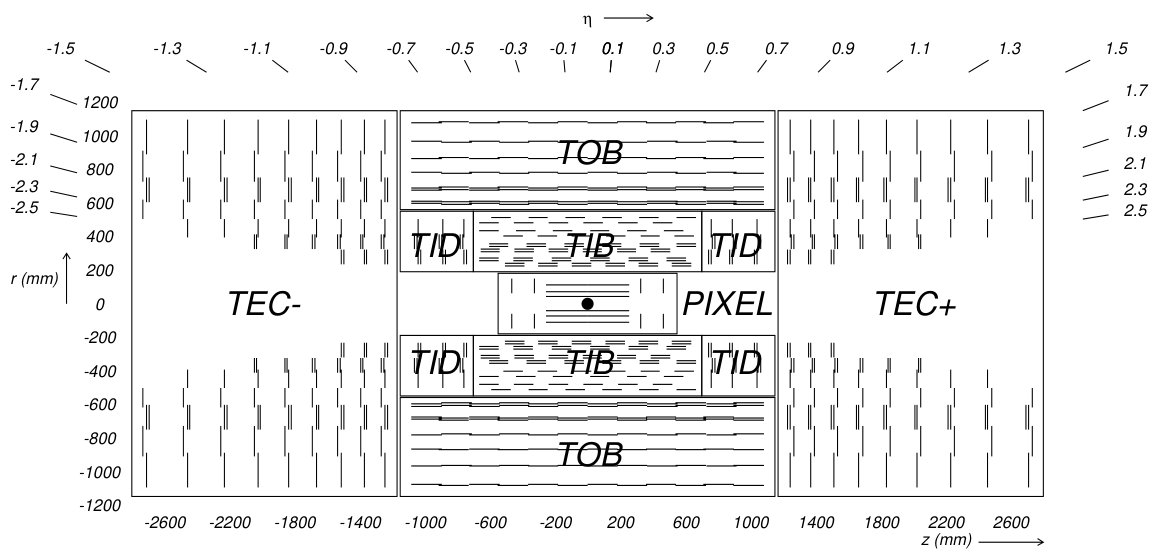
\includegraphics[width=0.9 \textwidth, ext=.png type=jpg]{/home/kpapad/UG_thesis/Thesis/Dissertation/src/figures/cms_tracker.jpg }
\caption{Schemtic illustration of a crossection of the CMS Tracker }
\label{fig:si_tracker}
\end{figure}


A schematic representation of the Sillicon Tracker's corss section, can be viewed on figure \ref{fig:si_tracker}. The tracker consists of a silicon pixel detector and a silicon strip detector. The silicon pixel detector is composed of two sub-detectors. Namely, the barrel which consists of three layers covering the region \(|\eta| < 2.2\) and at \(r = 4.4\text{, }7.3\text{ and }10,2\text{cm}\). The end caps, are two discs of pixel modues, located one on each side, that complete the design of the silicon pixel detector. The pixel detector improrves the trajectory and position measurements, by providing two-dimensional measurements of the charged particles' hit positions. (\href{https://cds.cern.ch/record/1129810}{source}).

The silicon strip detector, covers the radial region \(r \in \left[ 20, 116 \right]\text{cm}\). and  is comprised of four inner barrel (TIB) layers and two inner endcaps (TID). The TIBs are assembled in shells and each TID consists of three small discs. The outer barrel (TOB) encompasses both TIB and TID and contains six concentric layers. The tracker is closed off on either end by two endcaps (TEC). Measurements at the silicon strip detector give information regarding the path of each particle allows the distinction of separate particle trajectories.

\subsubsection{Energy Measurements: Calorimeters}
\label{sec:orgeca8eed}
Apart from measuring position and momentum, determining the energy of particles produced in LHC collisions is crucial. In the Compact Muon Solenoid (CMS) experiment, this information is obtained from particle interactions with matter in the calorimeters. Particles that are stable enough to reach the detector without decaying are either leptons, photons, or hadrons. The interactions between electrons, photons, and matter are of electromagnetic nature, while those between hadrons (charged or neutral) and matter are strong interactions. Therefore, the CMS experiment employs two types of calorimeters: the Electromagnetic Calorimeter (ECAL), located at the innermost layer, which measures the energy of photons and electrons, and the Hadron Calorimeter (HCAL), situated at the outer shells of the calorimeter section.

\begin{itemize}
\item Electromagnetic Calorimeter (ECAL)
\label{sec:org54126fa}

Figure \ref{fig:cms_ecal}(\href{https://www.slideserve.com/mac/requirements-and-status-of-the-cms-ecal-calorimeter}{source}) provides a view of the Electromagnetic calorimeters inside the CMS. The ECAL is composed of lead tungstate (PbWO4) crystals and is designed with a central barrel section (EB) and two endcaps (EE) that cover a range of pseudorapidities up to \(1.48\leq|\eta| \leq 3.0\)(\href{https://iopscience.iop.org/article/10.1088/1742-6596/587/1/012001}{source}). The crystals are highly dense and scintillate when high-energy photons or electrons interact with them. When a particle passes through the ECAL, it deposits its energy in the form of electromagnetic showers, which cause the crystals to emit light. The emitted light is then captured and amplified in order to estimate the energy of the incoming particle. The high-density crystals of the ECAL make it possible to accurately measure the energy of photons and electrons with high precision and resolution. 

\begin{figure}[ht]
\centering
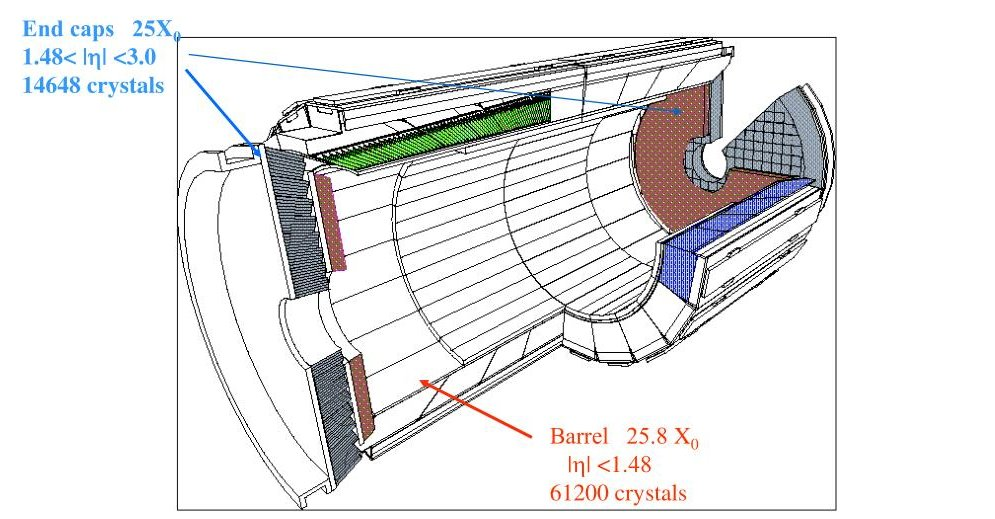
\includegraphics[width=0.9 \textwidth, ext=.png type=jpg]{/home/kpapad/UG_thesis/Thesis/Dissertation/src/figures/cms_ecal.jpg }
\caption{Schemtic illustration of the Ecal parts inside CMS }
\label{fig:cms_ecal}
\end{figure}


\item Hadron Clorimeter (HCAL)
\label{sec:orgbfeffb5}

The hadrons that manage to reach the detector, fly off the ECAl and interact with the Hadron Calorimeter. The HCAL consists of alternating layers of absorber material and plastic scintillator tiles that detect particles generated by the hadrons as they interact with the absorber.  When particles pass through the HCAL, they interact with the absorber material, producing showers of particles that create signals in the scintillator tiles. These signals are then read out and processed to measure the energy of the incoming hadrons. The HCAL has both a barrel section(HB), with pseudorapidity coverage at \(|\eta|<1.3\) and endcap(HE), covering a range of pseudorapidities \(1.3\leq|\eta| \leq 3.0\). The HCAL is highly effective at measuring the energy of hadrons due to its high-density absorber material and precise arrangement of scintillator tiles
(\href{https://www.slac.stanford.edu/econf/C060717/papers/L012.PDF}{source)}
\end{itemize}

\subsubsection{Detecting Muons}
\label{sec:org8c95f86}
In the outer regions of the CMS detectors, are located the muon chambers. They are the final part of the detector and are designed soley for the detection of muons, which due to their large mass(207 times greater than the electron mass) muons travel a longer distance in matter than electrons. Thus, their energy cannot be measured in ECAL. 

The muon chambers consist of 250 drift tubes (DTs) and 540 cathode strip chambers (CSCs), which track the positions of the particles. Additionally, there are 610 resistive plate chambers (RPCs) and 72 gas electron multiplier chambers (GEMs), making a total of 1400 chamber units . The use of multiple layers of detectors and different types of chambers makes the system robust and able to filter out background noise.

\begin{figure}[ht]
\centering
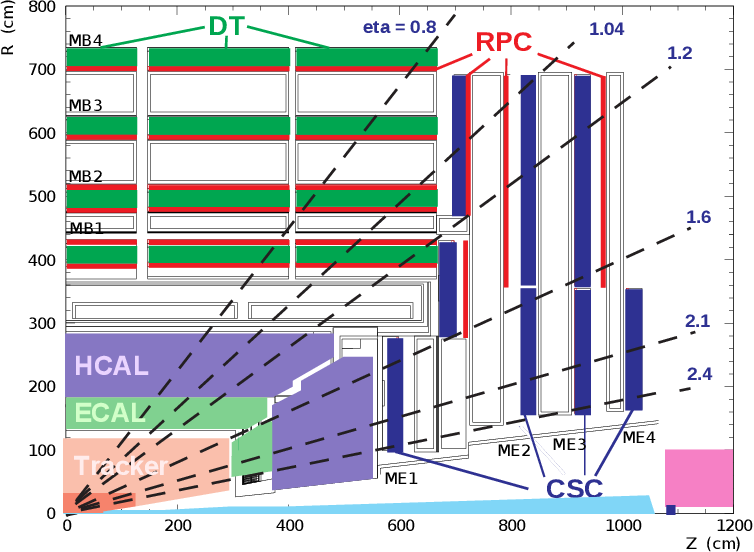
\includegraphics[width=0.9 \textwidth, ext=.png type=png]{/home/kpapad/UG_thesis/Thesis/Dissertation/src/figures/cms_MuonChambers.png }
\caption{A quarter sectional view of the CMS muon chambers. The beamline is perpendicular to the plane of the page}
\label{fig:muon_chambers}
\end{figure}

Figure \ref{fig:muon_chambers} illustrates the arrangement of the four different kinds of chambers. In the "barrel region," which surrounds the beam line, the DTs and square-shaped RPCs are grouped in coaxial cylinders. The CSCs, trapezoidal RPCs, and GEMs are located at the end cap region of the barrel . This arrangement allows for accurate measurements of the muons' trajectories and momenta in different regions of the detector.(\href{https://cms.cern/index.php/detector/detecting-muons}{source})

\section{Machine Learning for Classification}
\label{sec:org837d169}
The main goal Machine Learning is set to achieve, is the development of algorythms equiped with the capabillity of learning from data automatically. In particular, an artificially intelligent system must have the ability to identify objects in its surroundings, as well as anticipate the actions of its environment, in order to make informed decisions. Due to this, machine learning techniques tend to be more oriented towards forecasting, rather than prediction.
\subsection{Decision trees and Supervised Learning}
\label{sec:org9e96dfd}
The distinction between different particles, can be regarded as a classification problem where the target, is the prediction of a categorical output variable(i.e. lepton, boson), based on one or more input variables(i.e momenta components). Classification problems in  machine learning can be solved with supervised learning. In such procedure, a training data set is being used for the development(training) of a model that is able to perform the classification task. The output of the model is then beeing tested and evaluated on previously unseen data.

Before presenting any specific method of solving classification problems It is important to present an overview of the key elements in supervised learning.

\subsubsection{Supervised learning}
\label{sec:orgc2bcda3}
Let us pose the following problem:
Given a data set \(D= (\vec{X}, \vec{y})\), where \(\vec{X}\) is a matrix of the independet variables and \(\vec{y}\) is a vector of dependent variables, we want to find a model \(f(\vec{x} ; \vec{\theta})\),  that can predict an output from a set of input variables. Moreover, we  want to be able to judge the performance of the model on a given data set. To do that we need to define a cost function \(C(\vec{y}, f(\vec{X}; \vec{\theta}))\), such that the model will have to find the parameters \(\theta\) that minimize the cost function.\cite{Mehta_2019}

This the mathimatical pustulation of a supervised learning problem. I will now, in brief, discuss the role and interpretation of each of the 'ingredients' stated above.

\begin{itemize}
\item Model
\label{sec:org31e7a41}

The model, is a mathematical function \(f\text{ : } \vec{x} \rightarrow y\) of the parameters \(\theta\). Given a set of parameters, the output of the function, the prediction \(y_{i}\), is derived from the input variables \(\vec{x}\).
The parameters are undefined. The task of the training is to estimate the set of parameters from the training data set.
In a classification problem(something is of type a or it is not), it is possible to use the logistic transformation of the function output, to obtain the probability of the positive class.

\item Cost function
\label{sec:orgac31e22}

The cost function, also known as an objective function, is represented by mathematical function and it measures how well a model fits the training data. The cost function is used to train the model by finding the best set of parameters \(\theta\) that minimize the function.
In machine learning, the objective function, usually consists of two parts: a training loss function (L) and a regularization term (\(\Omega\)).

\[
obj(\theta) = L(\theta) + \Omega(\theta)
\]

The training loss function measures how predictive the model is with respect to the training data. A common choice of training loss function is the logistic loss, which is used for logistic regression(classification) and is given by

\[
L(\theta) = \sum_{i}[ y_{i}\ln(1+e^{-\hat{y_{i}}})+(1-y_{i}\ln(1+e^{\hat{y}_{i}}))]
\]
where \(y_{i}\) is the true label and \(\hat{y_{i}}\) is the predicted label.

The regularization term, \(\Omega(\theta)\), controls the complexity of the model, which helps to avoid overfitting. Overfitting occurs when a model is too complex and starts to extract local features from the training data. The model thus, looses its generalization power to new unseen data. Regularization helps to prevent overfitting by adding a penalty term to the cost function, which discourages the model from having too many parameters or too complex a structure.

The following figure gives an example of overfitting due to a very complex and very simple model.
\begin{center}
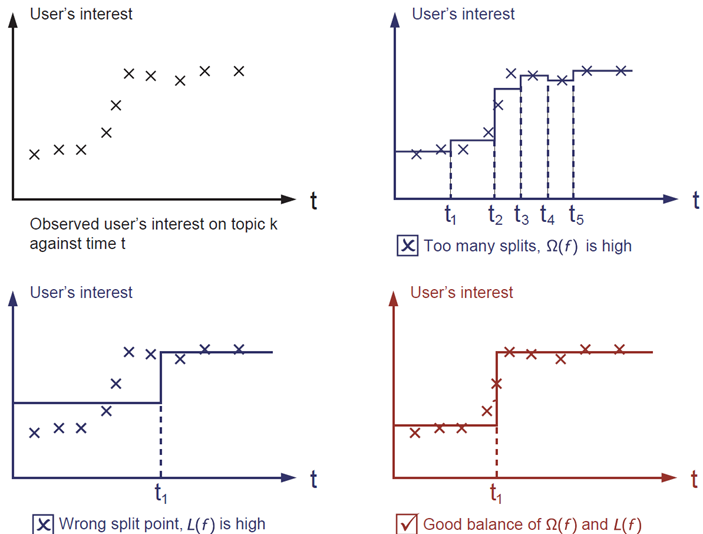
\includegraphics[width=.9\linewidth]{/home/kpapad/UG_thesis/Thesis/Dissertation/src/figures/boosted_trees_fig1.png}
\end{center}
\end{itemize}

\subsubsection{Decision Trees}
\label{sec:orgc68262f}
A decision tree is a flowchart-like tree structure, where each internal node represents a feature(or attribute), the branch represents a decision rule, and each leaf node represents the outcome.

Formally, a decision tree can be represented as a set of rules or conditions in the form of:

\texttt{f(X) = \{condition1, condition2,..condition\_n\}}

where each condition is a tuple of the form (feature, threshold, comparison operator) and the final outcome is represented by the leaf node.

For example, consider the decision tree of figure x that classify fruits based on color, shape, size, and taste. Let X be the input \texttt{X = \{"red", "smal", "sour"\}}. Then \texttt{f(X) = "grape"} 
\begin{center}
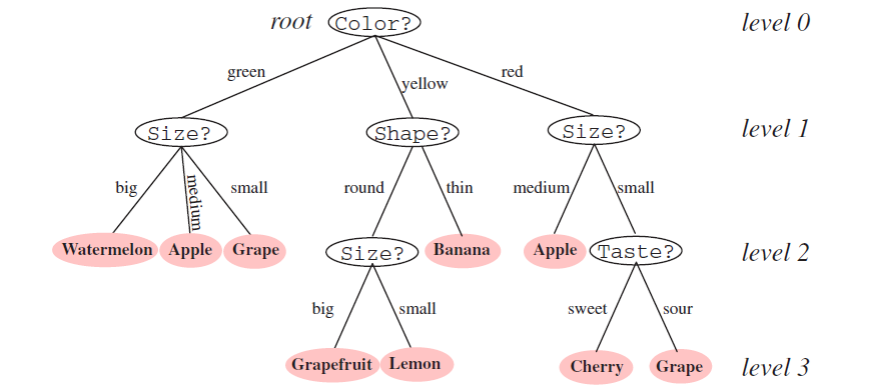
\includegraphics[width=.9\linewidth]{/home/kpapad/UG_thesis/Thesis/Dissertation/src/figures/boosted_trees_fig2.png}
\end{center} 

\begin{itemize}
\item Decision Tree Ensembles
\label{sec:org8a2fddb}

The tree ensemble model consists of a set of classification and regression trees (CART).
Let \(\mathcal{F}\) be the set of all possible CART's and \(f_{k} \in \mathcal{F}\), a function that represents a CART. The model in discussion then, can be written as:
\[
\hat{y_{i}} = \sum_{k=1}^{K} f_{k}(x_{i}),\text{ } f_{k} \in \mathcal{F}
\]

If \(\hat{y_{i}}\) represents the prediction of the tree, given an input variable \(x_{i}\), the real label of \(x_{i}\) will be denoted as \(y_{i}\)  . The objective function will be of the form:
\[
obj(\theta) = \sum_{i=1}^{n} l(y_{i}, \hat{y_{i}}) + \sum_{i=1}^{t}\omega(f_{i})
\]

where \(\omega(f_{i})\) is the complexity of a given tree  and l is the loss function.

\item Tree boosting
\label{sec:orgbee4670}

As stated earlier, the model is beeing trained, to learn those trees \(f_{k}\) that minimize the objective. The resulting model then, will be an ensemble of those functions \(f_{k}\).
The optimization of the objective, is a problem that cannot be solved with the traditional methods. Instead, the model is being iteratively trained in an additive manner.\cite{Chen_2016}
let the prediction value at the t-th iteration be \(\hat{y}^{(t)}_{i}\). In the next iteration(t+1), the chosen function \(f_{t+1}\), is such that if added to the model, the resulting prediction \(\hat{y}^{(t+1)}_{i}\) will minimize the cost function:
\[
\hat{y}^{(0)}_{i} = 0 \]
\[
\hat{y}^{(1)}_{i} =\hat{y}^{(0)}_{i} + f_{1}(x_{i}) 
\]
\[
\hat{y}^{(2)}_{i} =\hat{y}^{(1)}_{i} + f_{2}(x_{i}) 
\]

\[
\dots
\]
\[
\hat{y}_{i}^{(t)} = \hat{y}_{i}^{(t-1)} + f_{t}(x_{i})= \sum_{k=1}^{K} f_{k}(x_{i})
\]
The objective at step t is:
\[
obj^{(t)} = \sum_{i=1}^{n} l(y_{i}, \hat{y_{i}}^{(t)}) + \sum_{i=1}^{t}\omega(f_{i}) = \sum _{i=1}^{n} l(y_{i}, \hat{y}_{i}^{(t-1)} + f_{t}(x_{i})) + \omega(f_{i}(t))
\]

Taylor expanding the loss function \(l(y_{i}, \hat{y}_{i}^{(t-1)} + f_{t}(x_{i}))\), around \(f_{t}\), up to the second order and neglecting terms, referring to previous rounds, the specific objective becomes:

\[
\sum_{i=1}^{n}\left [ g_{i}f_{t}(x_{i})+\frac{1}{2}h_{i}f^{2}_{t} (x_{i}) \right ] + \omega(f_{t})
\]

Where
\[
g_{i} = \partial_{\hat{y}_{i}^{(t-1) }} l(y_{i}, \hat{y}_{i}^{(t-1)} )
\]
\[
h_{i} = \partial^{2}_{\hat{y}_{i}^{(t-1) }} l(y_{i}, \hat{y}_{i}^{(t-1)} )
\]

This is the minimization goal for \(f_{t}\) . \cite{xgboost}
\end{itemize}

\chapter{Search for heavy \(Y \rightarrow XX\)}
\label{sec:org96b6be0}
\label{sec:Search_Y_to_XX}
\section{The \(Y \rightarrow XX\)channel}
\label{sec:org0fd1492}
\label{sec:The_YtoXX_channel}
The \(Y \rightarrow XX\) dataset is composed of simulated events that represent the generic process of a resonance Y decaying into an XX pair, in the mass range between 100 and 300 GeV. The background consists of 50,839 events, while the signal comprises 5,946 events. The particular set is made up of miscellaneous pre-existing Monte Carlo (MC) samples, and the selected events contain only leptonic final states (one lepton and one antilepton of the same flavor). For the purpose of this study, only generator-level events were used, and given that we are not interested in any particular process, but rather in the most general case, no kinematic constraints were placed in the event selection. It should be noted that despite the fact that the parent MC samples contain lepton pairs in the final states, the resulting set can represent any diobject production in the selected mass range. The following table summarizes the features of the dataset in question:

\begin{table}[h!]
\centering
\begin{tabular}{ |p{3cm}|p{10cm}|  }
 \hline
Feature & Description \\
 \hline
$Pt_{1}$ &  The transverse momentum of the first particle in the XX pair \\
 \hline
$\eta_{1}$ &  The psudorapidity of the first particle in the XX pair \\
 \hline
$\phi_{1}$ &   azimuth angle of the first particle in the XX pair \\
 \hline
$Pt_{2}$ &  The transverse momentum of the second particle in the XX pair \\
 \hline
$\eta_{2}$ &  The psudorapidity of the second particle in the XX pair \\
 \hline
$\phi_{2}$ &   azimuth angle of the second particle in the XX pair \\
 \hline
\end{tabular}
\caption{Summary of the data set features }
\label{table:DataSetFeatures}
\end{table}

The mass spectrum for the \(Y \rightarrow XX\) decay, can be seen in figure \ref{fig:diX}

\begin{figure}[h]
\centering
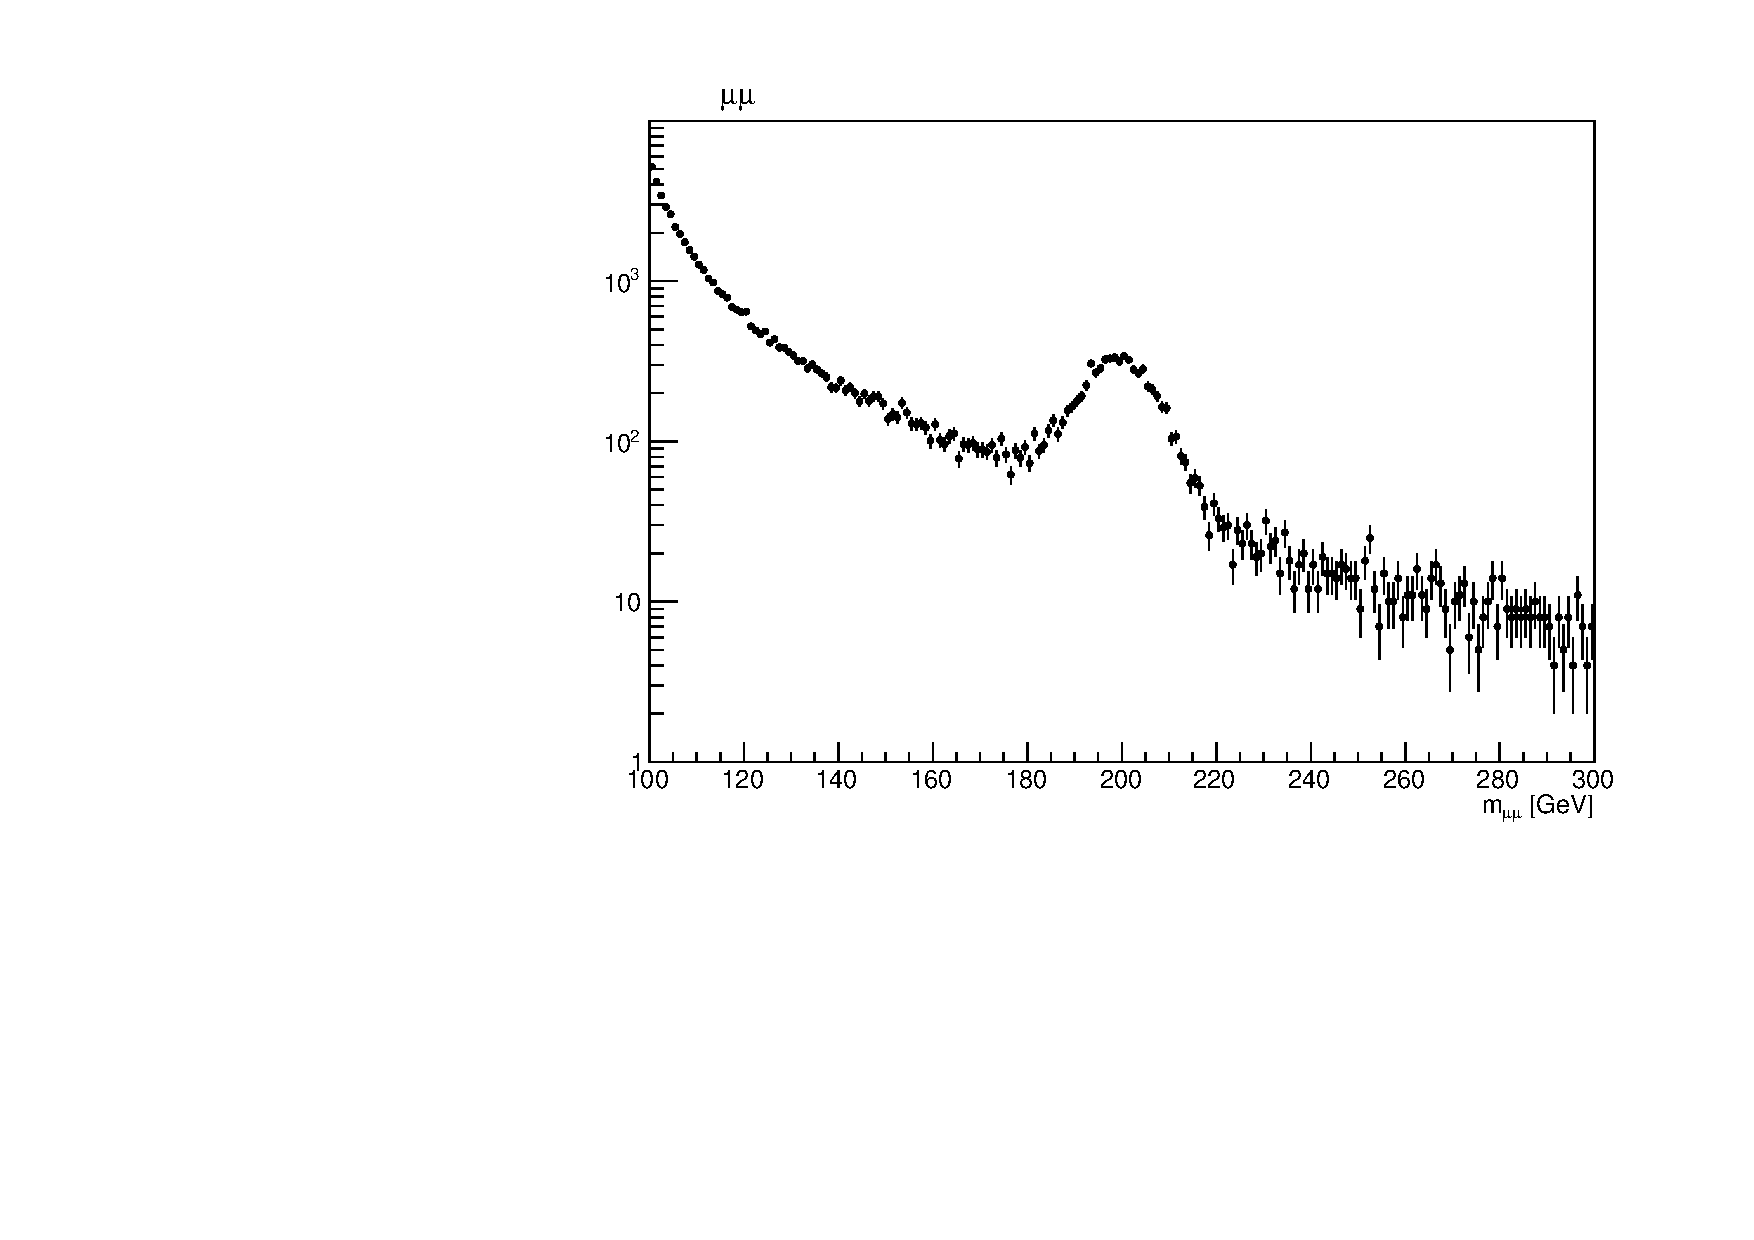
\includegraphics[width=0.5 \textwidth]{/home/kpapad/UG_thesis/Thesis/Analysis/out/Plots/DYJets_test2.pdf}
\caption{The $Y\rightarrow XX$ invariant mass spectrum}
\label{fig:diX}
\end{figure}

\section{Energy scale uncertainties}
\label{sec:org37b0e2d}
\label{sec:Energy_scale_uncertainties}
Energy scale uncertainties have an effect on the transverse momenta \(P_t\) of the produced \(XX\) pair. Such uncertainties are modeled as random noise (Gaussian smearing) to the signal component. To smear the data by \(x\%\), we iterate over every signal event and multiply the transverse momenta by numbers sampled from a Gaussian distribution of \(\mu = 1\) and \(\sigma = x/100\)(each \(P_t\) is multiplied by a different number).

In the present study, we compare the performance of a BDT-based analysis and a fit-based analysis on a given dataset, for various cases of smearing (various values of \(\sigma\)). Table \ref{table:Smearings} summarizes the smearing percentages used for this analysis. The values are chosen such that we examine both cases of mild noise (\(0-5\%\)) up to extreme noise (\(50\%\)). Nevertheless, it should be noted that what is considered as an extreme case or a mild case of smearing is not defined in an absolute manner but rather is related to the mass range of the data upon which the blur is applied.

\begin{table}[h!]
\centering
\begin{tabular}{ |c|  }
 \hline
Percentage of smearing \\
 \hline
$0\%$\\
$5\%$\\
$10\%$\\
$15\%$\\
$20\%$\\
$30\%$\\
$40\%$\\
$50\%$\\
\hline
\end{tabular}
\caption{Summary of the smearing cases that will be studied in this work }
\label{table:Smearings}
\end{table}

\section{Analysis Method I: Training a BDT Classifier}
\label{sec:org2ab78e2}
\label{sec:Analysis_method1}
\subsection{The Train/Test/Application data sets}
\label{sec:orgdba9d84}
\label{sec:Train_test_application_sets}
For the BDT training (and due to the lack of an infinite number of events), the original dataset had to be split into three parts. The training set is used to train the classifier. As the reader may have noticed, the signal events in the original dataset are much less than the background events. This class imbalance makes the training of the model much harder, and for that reason, the training set has been enriched with more (unseen) signal events, so that the two classes have the same number of events. The testing set is used to evaluate the training. For that purpose, the two signal and background classes also have the same number of events. Finally, the application set is used for the analysis. Through trial and error, we noticed that working with smaller statistics enhances the magnitude of statistical fluctuations in the analysis. To avoid such confusion, the application set contains a part of the testing set to ensure large statistics. This doesn't interfere with the training, since the BDT has never seen the testing events during training. Finally, it should be mentioned that in order to have an "apples-to-apples" comparison between the BDT-based analysis and the Fit-based analysis, the application set will be analyzed in both cases. For that reason, the smearing cases that will be discussed for the rest of this chapter will concern only the application set.

Table \ref{table:TrainTestApp} summarizes the number of events used in each dataset.

\begin{table}[h!]
\centering
\begin{tabular}{ |p{3cm}|p{3cm}|p{4cm}|  }
 \hline
Data Set & No.Signal Events & No. Background Events \\
 \hline
Training & 3882 & 3882 \\
Testing & 3881 & 3881 \\
Application & 2973 & 20827 \\
 \hline
\end{tabular}
\caption{Sumarry of the Train Test Application number of events}
\label{table:TrainTestApp}
\end{table}
\subsection{Training}
\label{sec:org02a9777}
\label{sec:Training}
One of the key aspects of a successful training is the feature space that is being used. Although the Train/Test sets consist of the features described in Table \ref{table:DataSetFeatures}, those features are not optimal for the particular classification problem. The feature space that is found to be optimal for the problem in question consists of five features and is summarized in Table \ref{table:TrainFeatures} and Figure \ref{fig:TrainFeaturesPlot}.

\begin{table}[h!]
\centering
\begin{tabular}{ |p{3.5cm}|p{11cm}| }
 \hline
Feature & Description \\
 \hline
$Pt_{1}$ &  the transverse momentum of the first particle in the XX pair. \\
 \hline
$Pt_{2}$ &the transverse momentum of the second particle in the XX pair. \\
 \hline
$\Delta\phi = \phi_{2} - \phi_{1}$ & the difference in the azimuthal angles between the two particles in the XX pair. \\
 \hline
$\Delta\eta = \eta_{2} - \eta_{1}$ & the difference in the pseudorapidity values between the two particles in the XX pair. \\
 \hline
$\Delta R = \sqrt{\Delta\eta^{2} + \Delta\phi^{2}}$ & the separation in the eta-phi plane between the two particles in the XX pair. \\
 \hline
\end{tabular}
\caption{Sumarry of the features used for training }
\label{table:TrainFeatures}
\end{table}

\begin{figure}[h!]
\centering
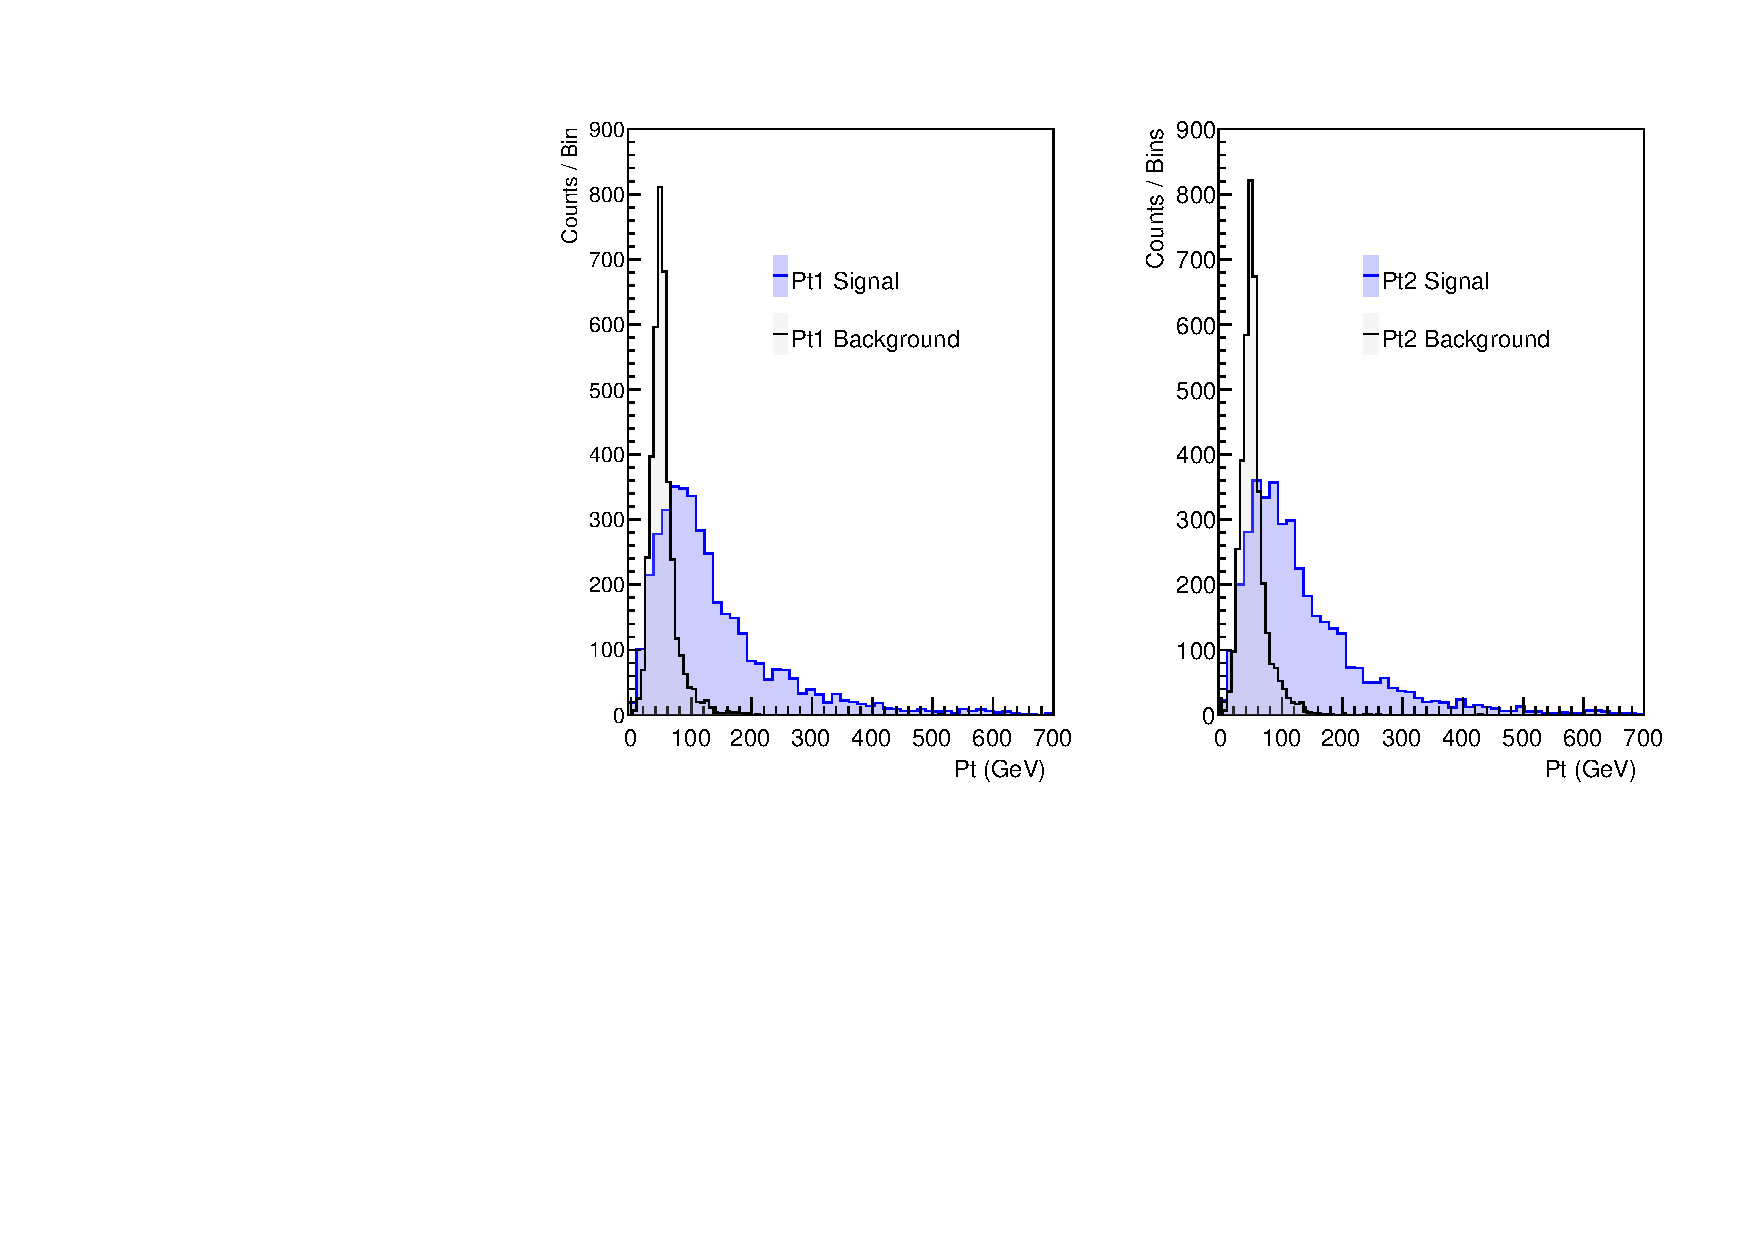
\includegraphics[page=1,width=\textwidth]{/home/kpapad/UG_thesis/Thesis/Analysis/out/Plots/WPhiJets_M200M100300Deltas_varsplot.pdf}
\includegraphics[page=2,width=\textwidth]{/home/kpapad/UG_thesis/Thesis/Analysis/out/Plots/WPhiJets_M200M100300Deltas_varsplot.pdf}
\caption{Sumarry of the features used for training }
\label{fig:TrainFeaturesPlot}
\end{figure}

To assess the performance of the trained model, the Area Under the Receiver Operating Curve (ROC-AUC) is used as a metric. However, it is important to note that in addition to evaluating the model's performance, we also consider the possibility of overfitting. To quantify overfitting, we examine the ratio of the number of training events to the number of testing events at a particular BDT score. If the model is not overtrained, the performance on the training and testing set will be approximately the same, and therefore, the ratio will fluctuate around 1 across the BDT score range.

Figure \ref{fig:BDTplot} displays the BDT score plot of the training and testing set, as well as the corresponding ROC curves. The performance of the model on the testing set yields an AUC score of 0.98. Looking at the Training/Testing ratios, one can notice that they fluctuate around one. The absence of a profound trend in both signal and background ratios implies that the model is not severely overfitted.
\begin{figure}[h!]
\centering
\begin{subfigure}{0.49\textwidth}
\centering
\includegraphics[page=5, width=\linewidth]{/home/kpapad/UG_thesis/Thesis/Bdt/out/Plots/WPhiJets_M200M100300DeltasPConf12BDTplot.pdf}
\caption{}
\end{subfigure}
\begin{subfigure}{0.49\textwidth}
\centering
\includegraphics[page=3, width=\linewidth]{/home/kpapad/UG_thesis/Thesis/Bdt/out/Plots/WPhiJets_M200M100300DeltasPConf12BDTplot.pdf}
\caption{}
\end{subfigure}
\caption{A: The BDT score of the Testing and Training sets. B: The roc curves for the training and testing sets}
\label{fig:BDTplot}
\end{figure}
\newpage
\subsection{Application}
\label{sec:orgf09d0f1}
\label{sec:Application}
The application of the model to the application set is a rather straightforward process. The data are simply "fed" to the model, and the latter performs the classification. The ROC curves for the performance of the trained model on the data for each of the smearing cases of table \ref{table:Smearings} are illustrated in figure \ref{subfig:SmearingROC}.

\begin{figure}[h]
\centering
\begin{subfigure}{0.49\textwidth}
\centering
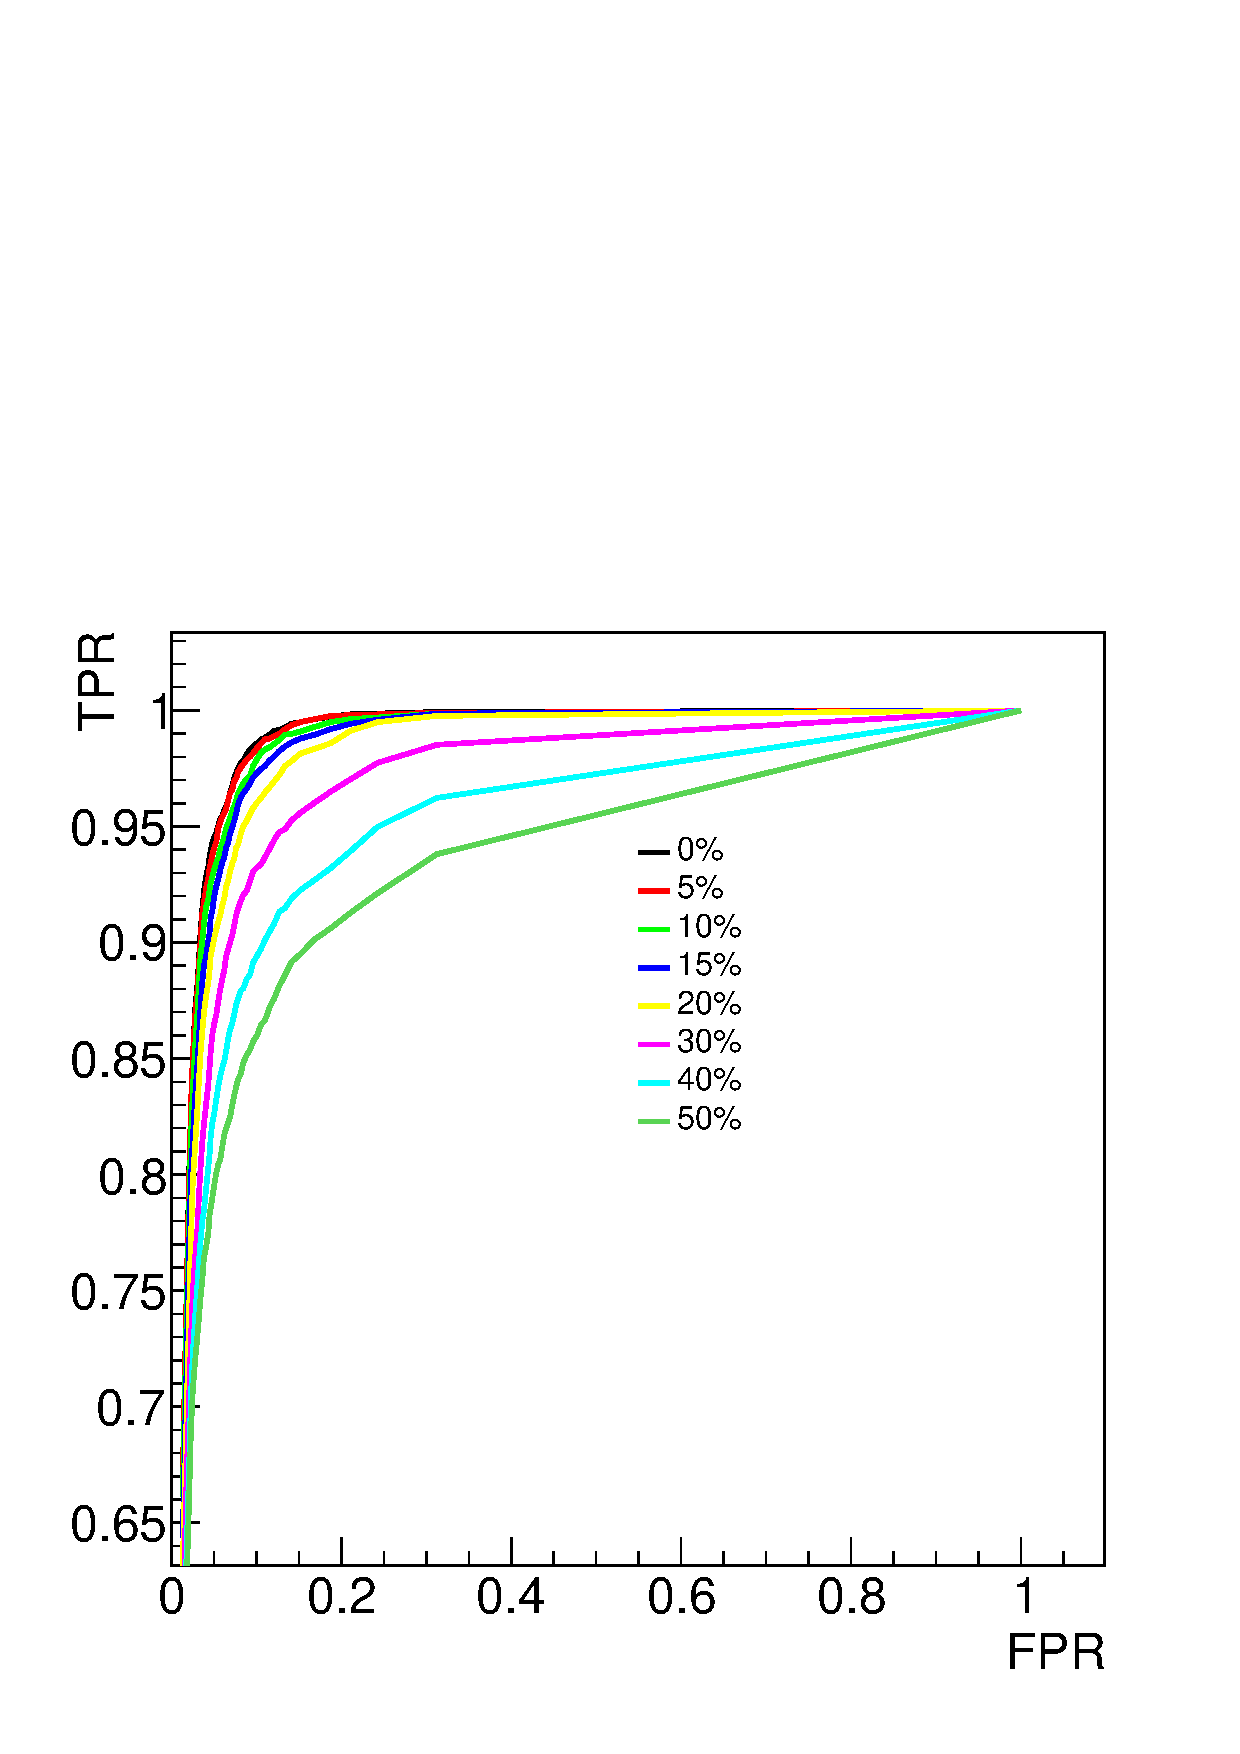
\includegraphics[page=1,width=\linewidth]{/home/kpapad/UG_thesis/Thesis/Bdt/src/WPhiJets_M200M100300_ROCs.pdf}
\caption{}
\label{subfig:SmearingROC}
\end{subfigure}
\begin{subfigure}{0.49\textwidth}
\centering
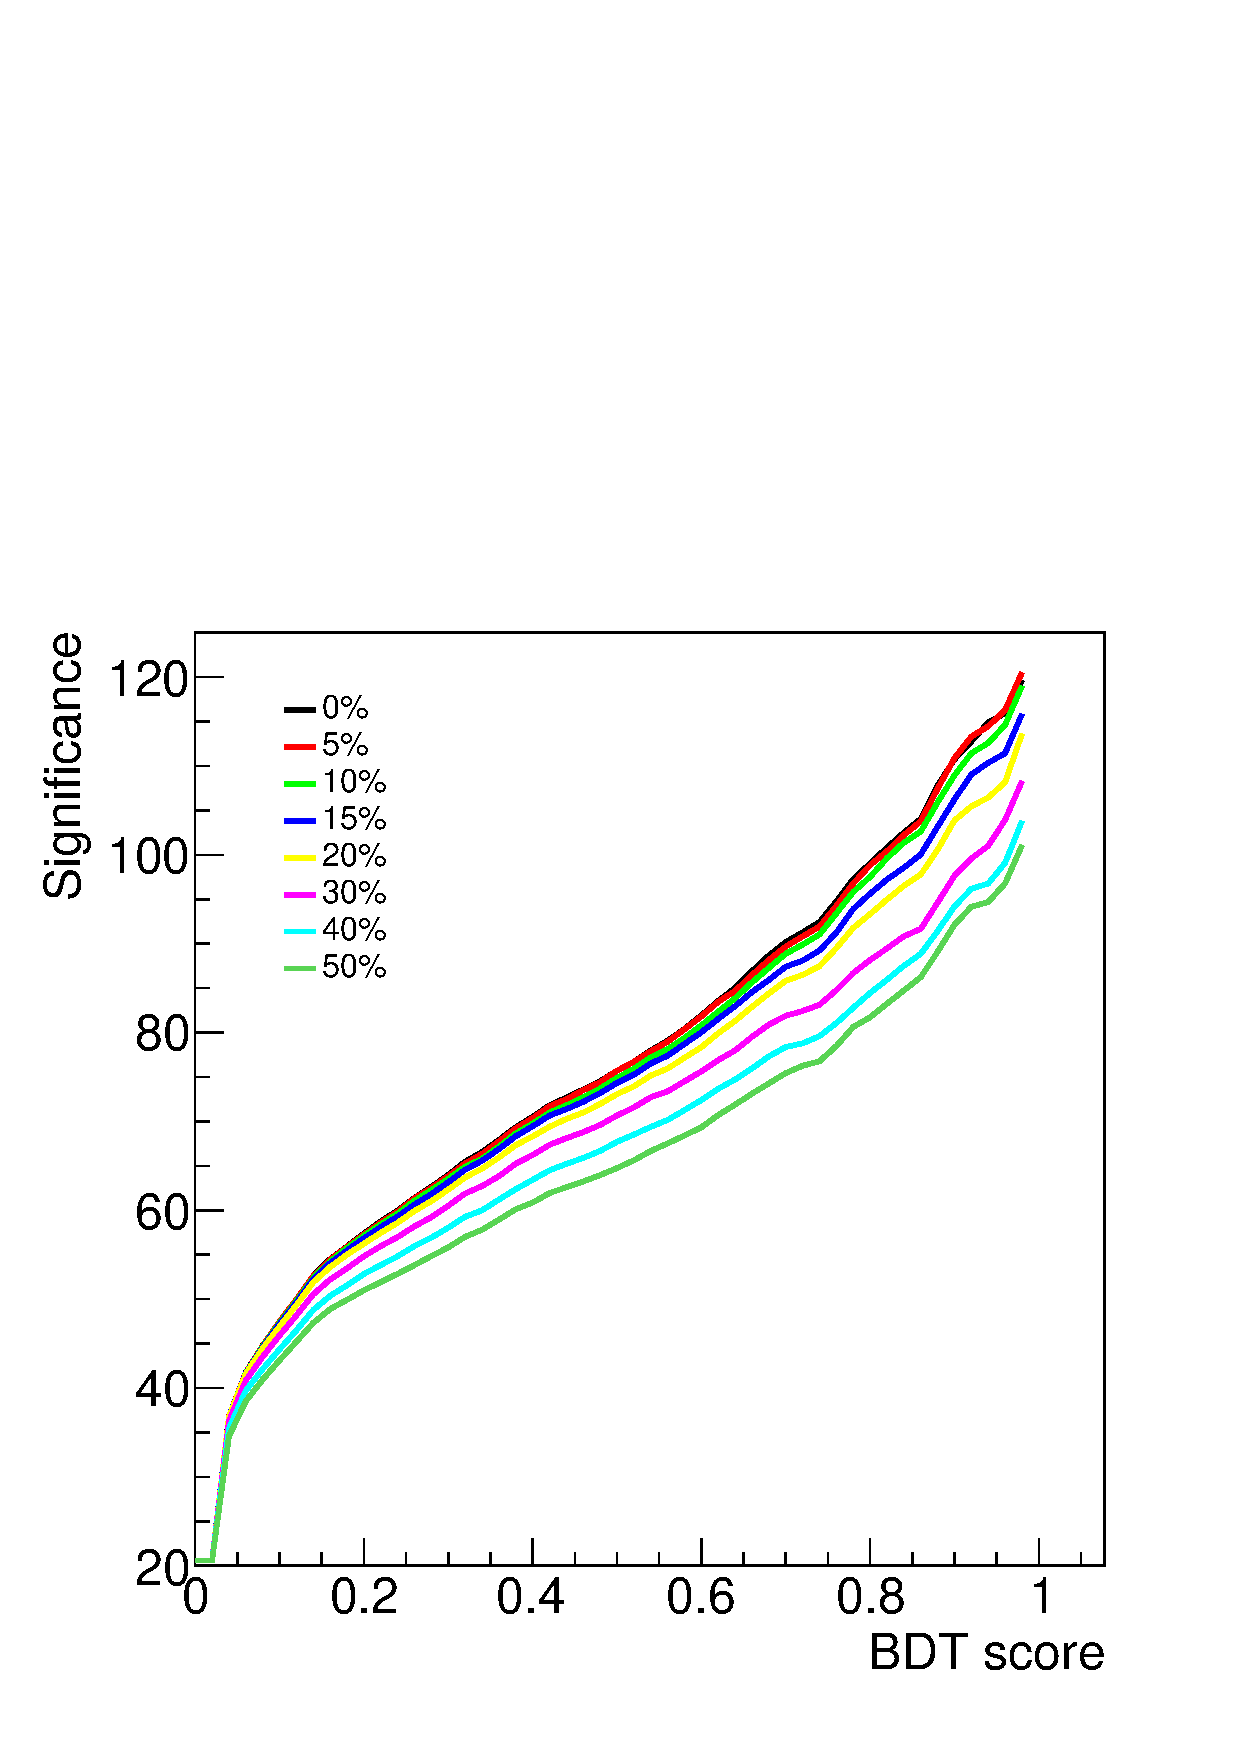
\includegraphics[page=1,width=\linewidth]{/home/kpapad/UG_thesis/Thesis/Bdt/src/WPhiJets_M200M100300_Significance.pdf}
\caption{}
\label{subfig:SigScan}
\end{subfigure}
\caption{a: Summary of the ROC curves for the performance of the model on the data for each smearing case. b: Significances calculated across the BDT score range for the smearing cases of Table \ref{table:Smearings}. The way that these curves are made is analogous to the calculation of the ROC curve.}
\end{figure}

To find the optimal BDT score to place the cut, the whole BDT score range is scanned, and the significance is evaluated in the range [c,1], \(\forall c\in[0,0.98]\) with step size 0.02, same as the bin width of the BDT score histogram(it is pointless to calculate the significance at a single point since it will be 0). The scan of significance for every case of smearing is illustrated in figure \ref{subfig:SigScan}.

Looking at the plot, the cut that gives the best significance is c = 0.98 (the region will be [0.98,1]). Moreover, it is of interest to consider a wider region as well, for the reason that more signal is accepted despite the rejection of less background. To make this argument a bit clearer, let us consider figure \ref{fig:BDTplot}a. At BDT score \textasciitilde{} 7 and onwards, the amount of background events in each bin remains somewhat constant (within statistical fluctuations) while the signal events increase rapidly. It is therefore interesting for our analysis to see how this behavior reflects on the evolution of significance for the various cases of smearing. Looking at figure \ref{subfig:SigScan} again, we conclude that a cut at c = 0.86 is good enough for our purpose.

The results can be seen in Figure \ref{fig:SigEvolBDT} which compares the evolution, in terms of smearing percentage, of the significance for the cuts c = 0.98 and c = 0.86. Table \ref{table:SigBkgBDT} presents the amount of signal and background events present for the two cuts.

\begin{figure}[h!]
\centering
\includegraphics[page=2,width=0.5\textwidth]{/home/kpapad/UG_thesis/Thesis/Bdt/src/WPhiJets_M200M100300_Significance.pdf}
\caption{Evolution of significance for the smearing cases of table \ref{table:Smearings}. }
\label{fig:SigEvolBDT}
\end{figure}


\begin{table}[ht]
\centering
\begin{tabular}{|p{2cm}|p{3cm}|p{3cm}|p{3cm}|p{3cm}|}
 \hline
Smearing \%  & No. Sig. Events at BDT cut = 0.86 & No. Bkg.Events at BDT cut = 0.86 & No. Sig. Events at BDT cut = 0.98 & No. Bkg.Events at BDT cut = 0.98  \\
\hline
0 & 2622.0 & 635.0 & 1977.0 & 273.0 \\
5 & 2615.0 & 635.0 & 1991.0  & 273.0 \\
10 & 2586.0 & 635.0 & 1966.0 & 273.0 \\
15 & 2521.0 & 635.0 & 1914.0 & 273.0 \\
20 & 2464.0 & 635.0 & 1877.0 & 273.0 \\
30 & 2310.0 & 635.0 & 1789.0 & 273.0 \\
40 & 2239.0 & 635.0 & 1715.0 & 273.0 \\
50 & 2173.0 & 635.0 & 1670.0 & 273.0 \\
 \hline
\end{tabular}
\caption{Signal and background events at BDT cut 0.86 and 0.98 for different smearing percentages.}
\label{table:SigBkgBDT}
\end{table}
\newpage
\clearpage
\section{Analysis Method II: Fit based analysis}
\label{sec:orgb3ebefa}
\label{sec:Analysis_method2}
\subsection{Invariant mass reconstruction}
\label{sec:org2532a44}
\label{sec:Invariant_mass_reconstruction}
The invariant mass of the XX pair is calculated using the features in Table \ref{table:DataSetFeatures}. The resulting spectrum is shown in Figure \ref{fig:AppMass}.

\begin{figure}[h!]
\centering
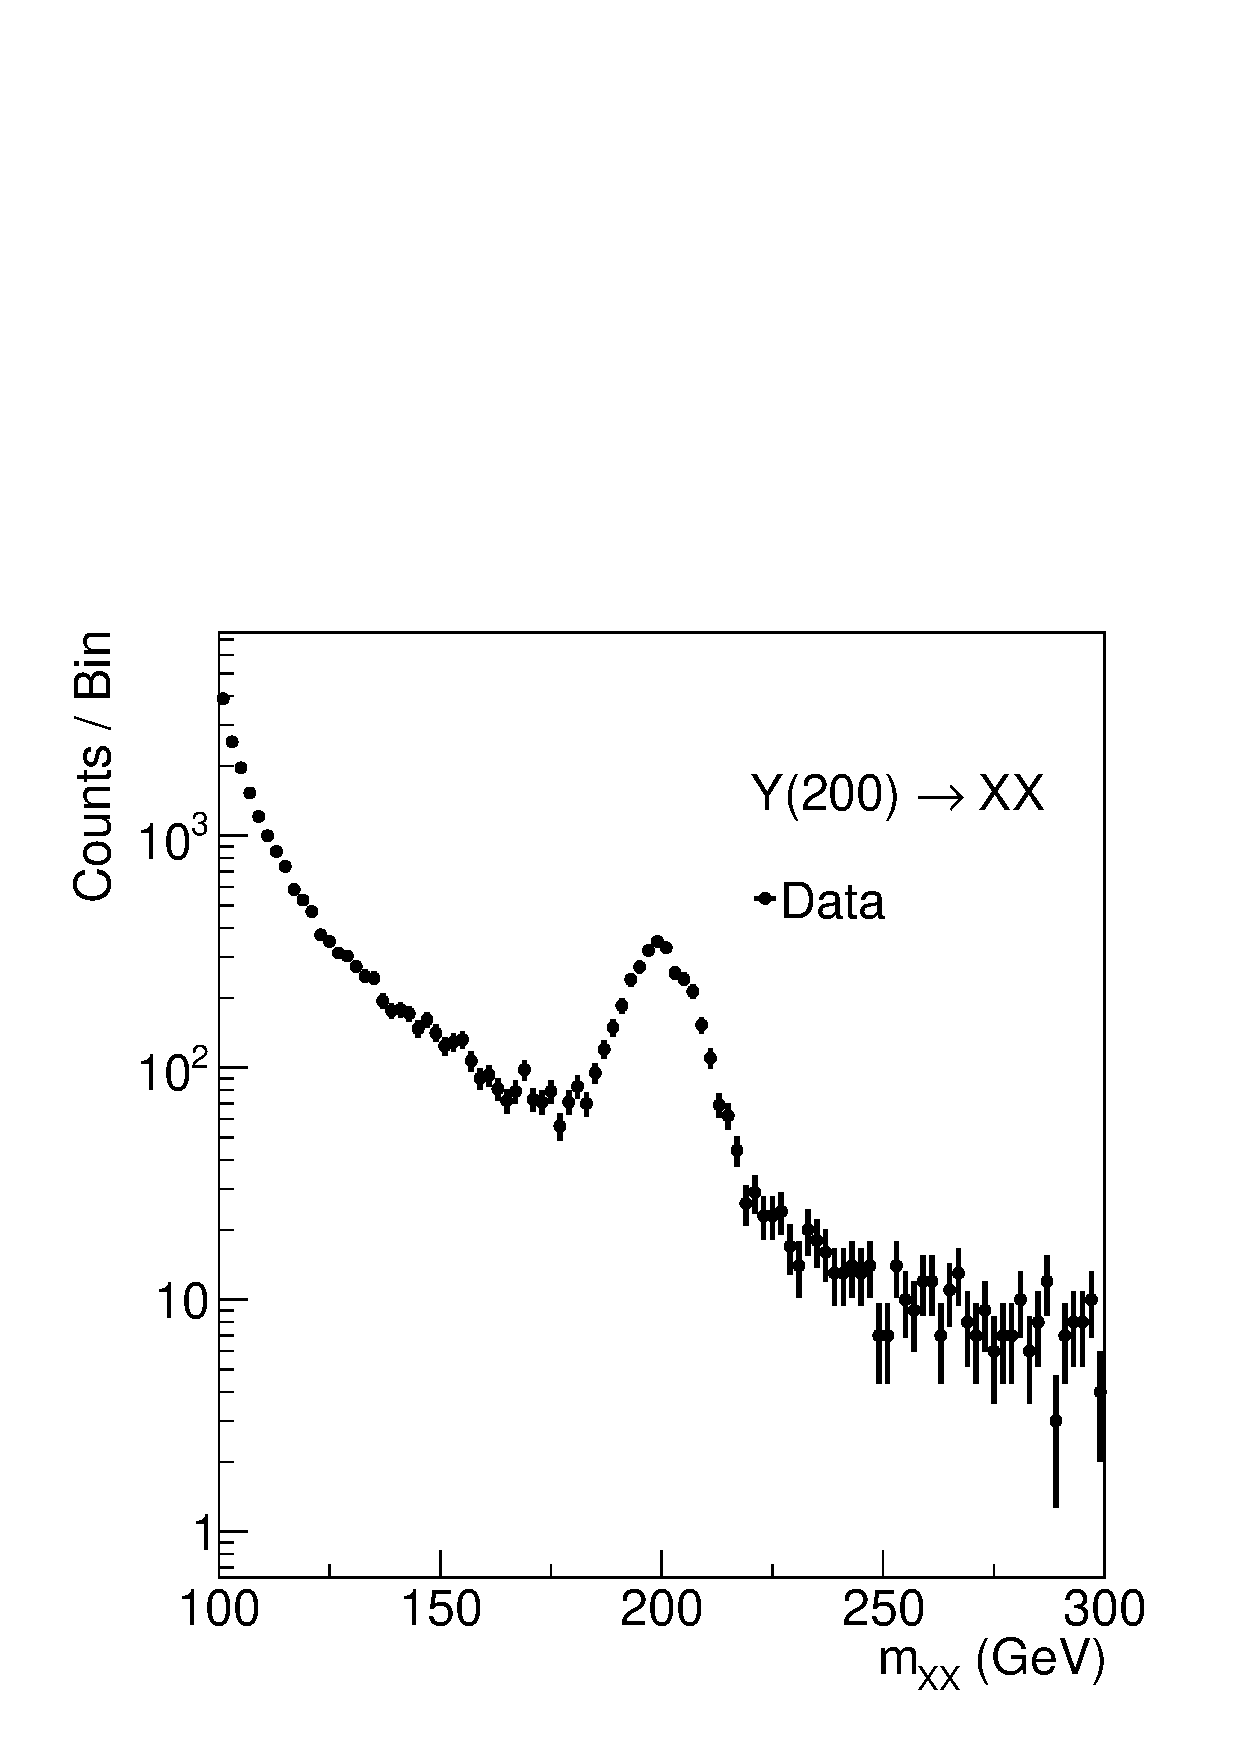
\includegraphics[page=1,width=0.5\textwidth]{/home/kpapad/UG_thesis/Thesis/Analysis/out/Plots/WPhiJets_M200M100300_Application_MassSpectrum.pdf}
\caption{The invariant mass spectrum of the application set}
\label{fig:AppMass}
\end{figure}

Events with invariant mass \(m_{XX} < 120\text{GeV}\) make the background fit significantly harder without contributing significantly to the analysis. Therefore, such events are excluded from this study, and the working mass spectrum is limited to the range \([120, 300]\text{GeV}\).
\subsection{Background Fitting}
\label{sec:org780d746}
\label{sec:Background_fitting}
As discussed in previous sections, the applied smearing only affects the signal component of the application set. For this reason, and to simplify the analysis, the background shape is fitted separately and kept constant throughout the signal fits.

Despite this simplification, determining the shape of the background was not a trivial process. Through trial and error, the function shown in Equation \ref{eq:bkgFitFunc} was found to be the best fit.
\begin{equation}
bkg(x) = \alpha + \beta x^{-1/2} + \gamma x^{-1} + \delta x^{3/2}
\label{eq:bkgFitFunc}
\end{equation}
The parameters \(\alpha\), \(\beta\), \(\gamma\), and \(\delta\) are free parameters of the fit. The modeled background is illustrated in Figure \ref{fig:BKGfit}.

\begin{figure}[h!]
\centering
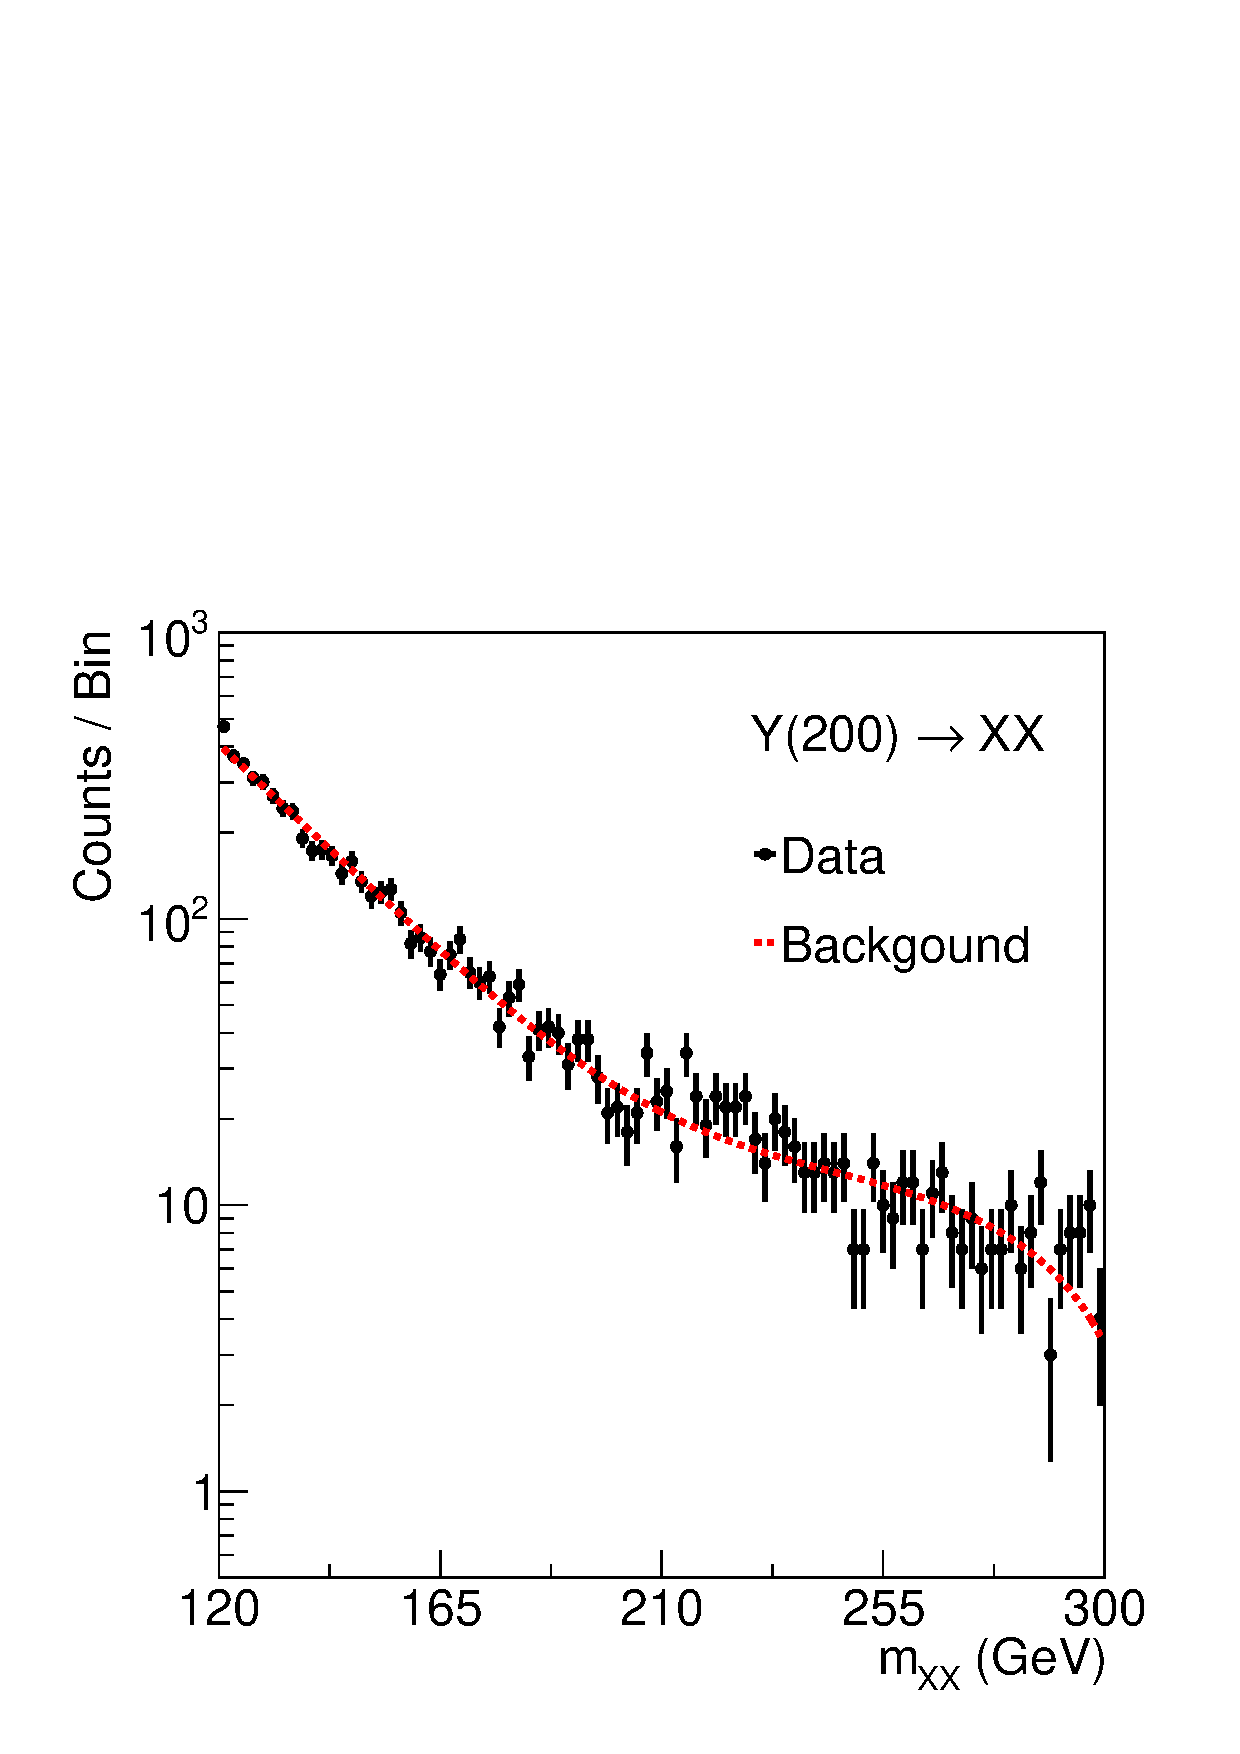
\includegraphics[page=1,width=0.5\textwidth]{/home/kpapad/UG_thesis/Thesis/Analysis/out/Plots/WPhiJets_M200M100300_Application_bkgFit.pdf}
\caption{The fitted background}
\label{fig:BKGfit}
\end{figure}
\subsection{Signal Fitting}
\label{sec:org3f69715}
\label{sec:Signal_fitting}
The signal is fitted using a Gaussian function with \(\sigma\) and magnitude as free parameters, and \(\mu = 200\text{GeV}\) (the mass of the resonance). Figure \ref{fig:fits} shows the fitted invariant mass spectra for smearing percentages of \(0\%\), \(5\%\), \(10\%\), \(15\%\), and \(20\%\). As illustrated in Figure \ref{fig:extremeSmearings}, the signal mass in the extreme cases of \(30\%\text{, }40\%\) and \(50\%\) smearing is indistinguishable from the background. Therefore, attempting to fit those spectra would be a pointless exercise.
\subsection{Signal from background separation}
\label{sec:orgec7f99c}
\label{sec:Signal_from_background_separation}
As with the BDT method, we want the region of interest that yields the best significance. To do so, we scan various mass windows around the center of the signal. We scanned six different regions (in the \(0\%\) case), beginning from \(\pm 0.5\sigma\) up to \(\pm 3\sigma\) with a step of \(0.5\sigma\). The results can be seen in Figure \ref{fig:Scan0}. It is evident that the region \(\pm 1.5\sigma\) provides the best performance in terms of significance.
\begin{figure}[h!]
\centering
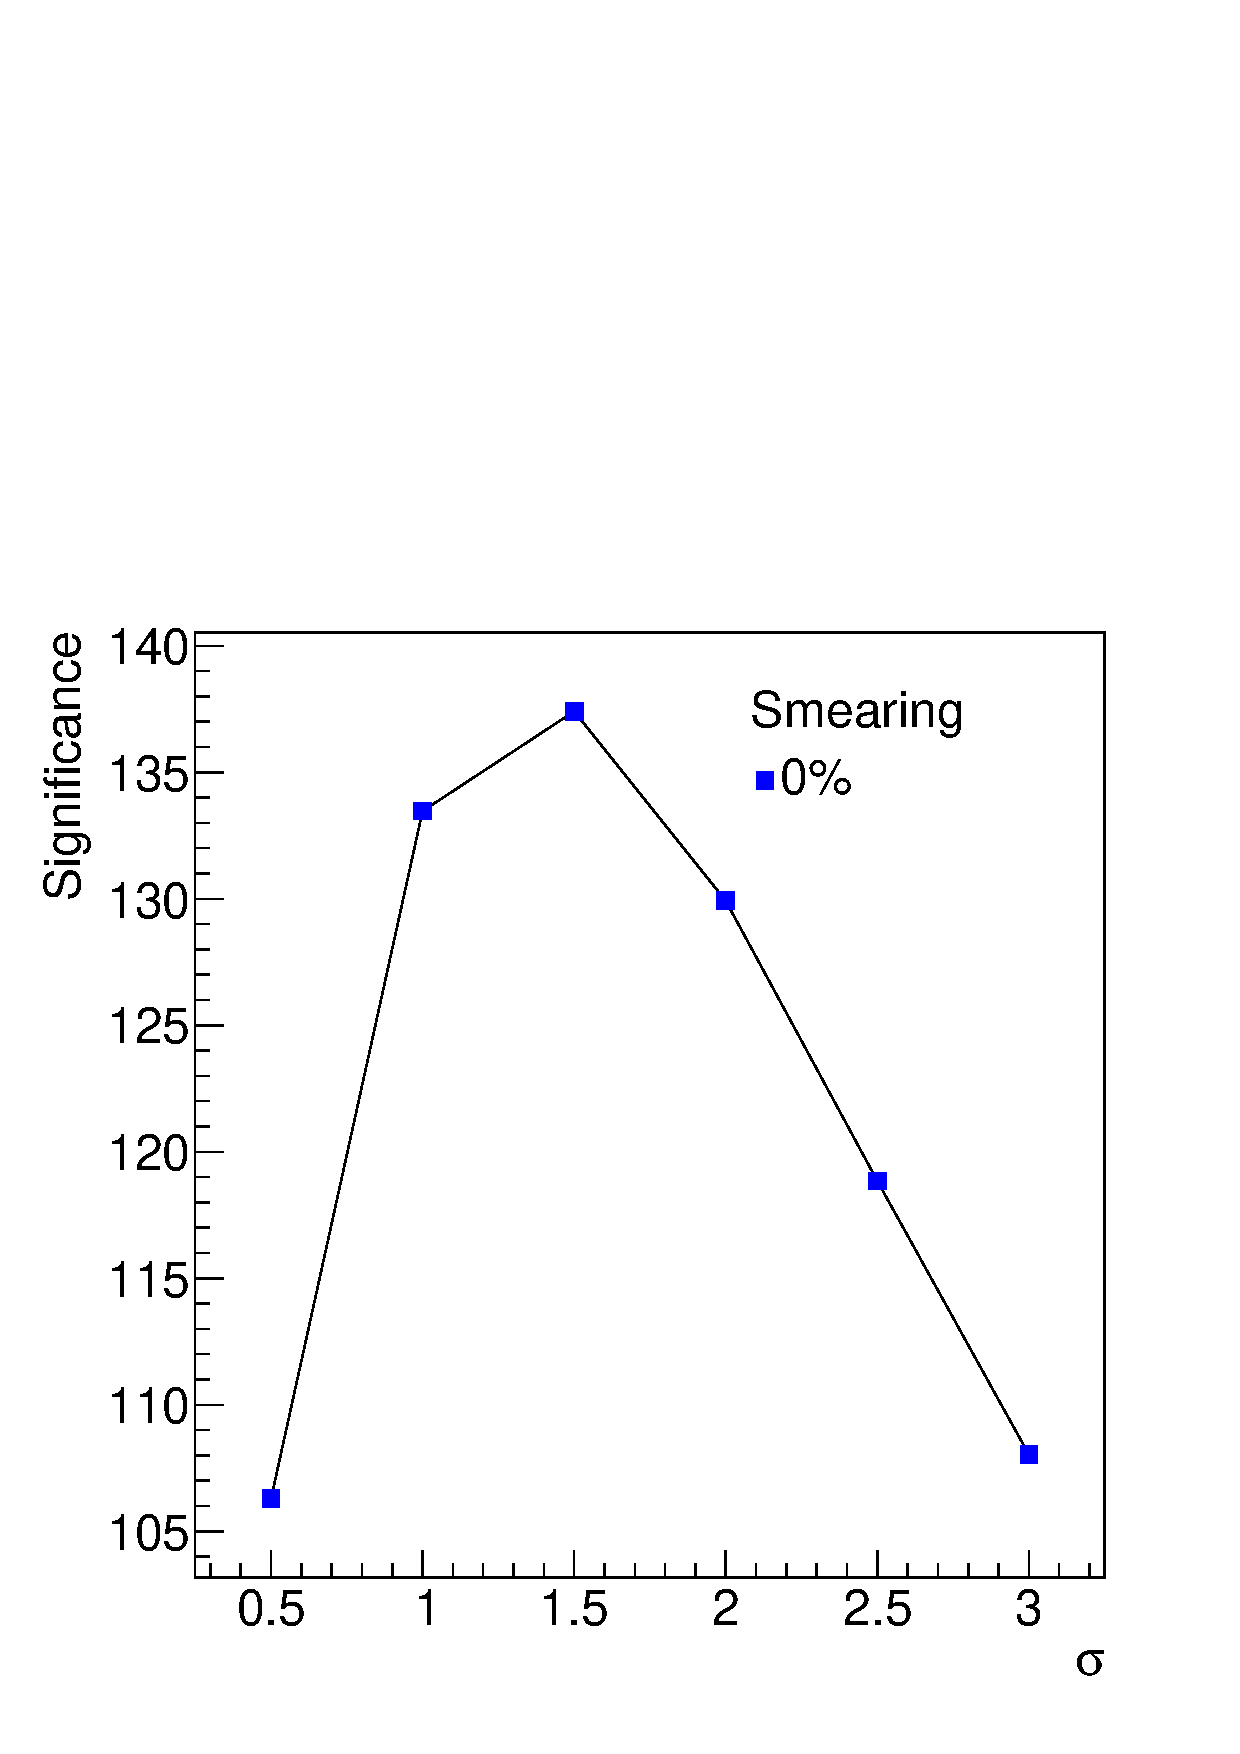
\includegraphics[page=1,width=0.5\textwidth]{/home/kpapad/UG_thesis/Thesis/Analysis/src/WPhiJets_M200M100300_Significance0.pdf}
\caption{Scan of significance for various values of $\sigma$, in the $0\%$ smearing case. We see that the regrion $\pm 1.5\sigma$ around $\mu=200GeV$, gives the best significance.}
\label{fig:Scan0}
\end{figure}

We can then study how the significance changes in the selected region for the various smearing cases in two ways, based on the interpretation of the \(\pm 1.5\sigma\) region. One can interpret \(\sigma\) as the Gaussian spread of the \(0\%\) case and calculate every significance value in the same mass window, resulting in a fixed window study. On the other hand, one can interpret \(\sigma\) as the Gaussian spread of each smearing case. That is, the significance will still be calculated at a \(\pm 1.5\sigma\), but the range will be different based on the different values of \(\sigma\) for every fit, resulting in an adaptive window study. For completeness, we did both studies, and the results are presented in Figure \ref{fig:AdaFixedSig}. Table \ref{table:AdaSigmas}, summarizes the the values of \(\sigma\) (resulting from the fits), and the corresponding mass window for the adaptive widnow search, while table \ref{table:NumSigBkg}, summarizes the amount of signal and background events present in the region of interest of both studies(fixed and adaptive window).
\begin{figure}[h!]
\centering
\includegraphics[page=3,width=0.5\textwidth]{/home/kpapad/UG_thesis/Thesis/Bdt/src/WPhiJets_M200M100300_Significance.pdf}
\caption{Copmarison of the significance evolution as caclulated in the fixed widow and adaptive window case.} 
\label{fig:AdaFixedSig}
\end{figure}
\begin{table}[htbp]
\centering
\begin{tabular}{|p{2cm}|p{2cm}|c|}
 \hline
Smearing \%  & $\sigma$ in GeV & Invarian Mass $\pm 1.5\sigma$ window  in GeV \\
\hline
0 & 7.62 & 23.01\\
5 & 11.15 & 33.47 \\ 
10 & 16.33 & 48.98 \\ 
15 & 22.90 & 68.70 \\ 
20 & 28.87 & 86.60 \\ 
 \hline
\end{tabular}
\caption{Summary of the invariant mass windows used used in adapitve window study. Note that the resulting window of $0\%$ smearing corresponds to the fixed window case as well.}
\label{table:AdaSigmas}
\end{table}
\begin{table}[h!]
\centering
\begin{tabular}{|p{2cm}|p{3cm}|p{3cm}|p{3cm}|p{3cm}|}
 \hline
Smearing \%  & No. Sig. Events (fixed window) & No. Bkg.Events (fixed window) & No. Sig. Events (adaptive window) & No. Bkg.Events (adaptive window)  \\
\hline
0 & 2426 & 311 & 2426 & 311 \\
5 & 2012 & 311 & 2506 & 476 \\
10 & 1511 & 311 & 2539 & 752 \\
15 & 1118 & 311 & 2524 & 1202 \\
20 & 884 & 311 & 2465 & 1662 \\
 \hline
\end{tabular}
\caption{Signal and background events in the 23Gev fixed window region and in the $\pm 1.5\sigma$ adaptive window region, for different smearing percentages.}
\label{table:NumSigBkg}
\end{table}

\section{Results}
\label{sec:orgacc4269}
So far, in sections \ref{sec:Analysis_method1} and \ref{sec:Analysis_method2}, we have studied how does a multivariate and a singlevariate calssifcation technique responds to energy scale uncertainties, in a signal from background sepparation task, in the heavy mass region. In this section, we are going to summarize the results and provide commentary regarding each method, in terms of performance and robustness. Moreover will will draw a comparizon between the two methods.

\begin{figure}[h!]
\centering
\includegraphics[page=4,width=0.5\textwidth]{/home/kpapad/UG_thesis/Thesis/Bdt/src/WPhiJets_M200M100300_Significance.pdf}
\caption{ Comparison of the perfomance of the BDT and Fit based analysis, in terms of sifnificance,  as a function of the smearing cases. We can see that BDT based analysis, is more robust.}
\label{fig:BdtFitSig}
\end{figure}

Figure \ref{fig:BdtFitSig}, compares the significance yielded by each method, as a function of smearing. 
Even though, at \(0\%\) of smearing, the fit based method, yields a better significance than the BDT method, the bdt is more robust in general. To explain this, on must pay close attention to the feature space used for the training. The classifier learns not only the energy related Pts of the X particles, but also the geometrical features, \(\Delta\phi\text{, }\Delta R\text{ and }\Delta\eta\). As discribed in section \ref{sec:Energy_scale_uncertainties}, smearing has an effect only on the Pt variables, while the spatial features remain invariant under such process. That is, the BDT model, learns to classify the signal, using features that do not change through out the smearing process, and is therefore able to deliver a better performance, when compared to the fit based analysis, which only makes use of the invariant mass, a feature that gets heavilly altered by uncertainties on the energy scale as figures \ref{fig:fits} and \ref{fig:extremeSmearings} indicate. 

\begin{figure}[hbpt]
\centering
\begin{subfigure}{0.45\textwidth}
\centering
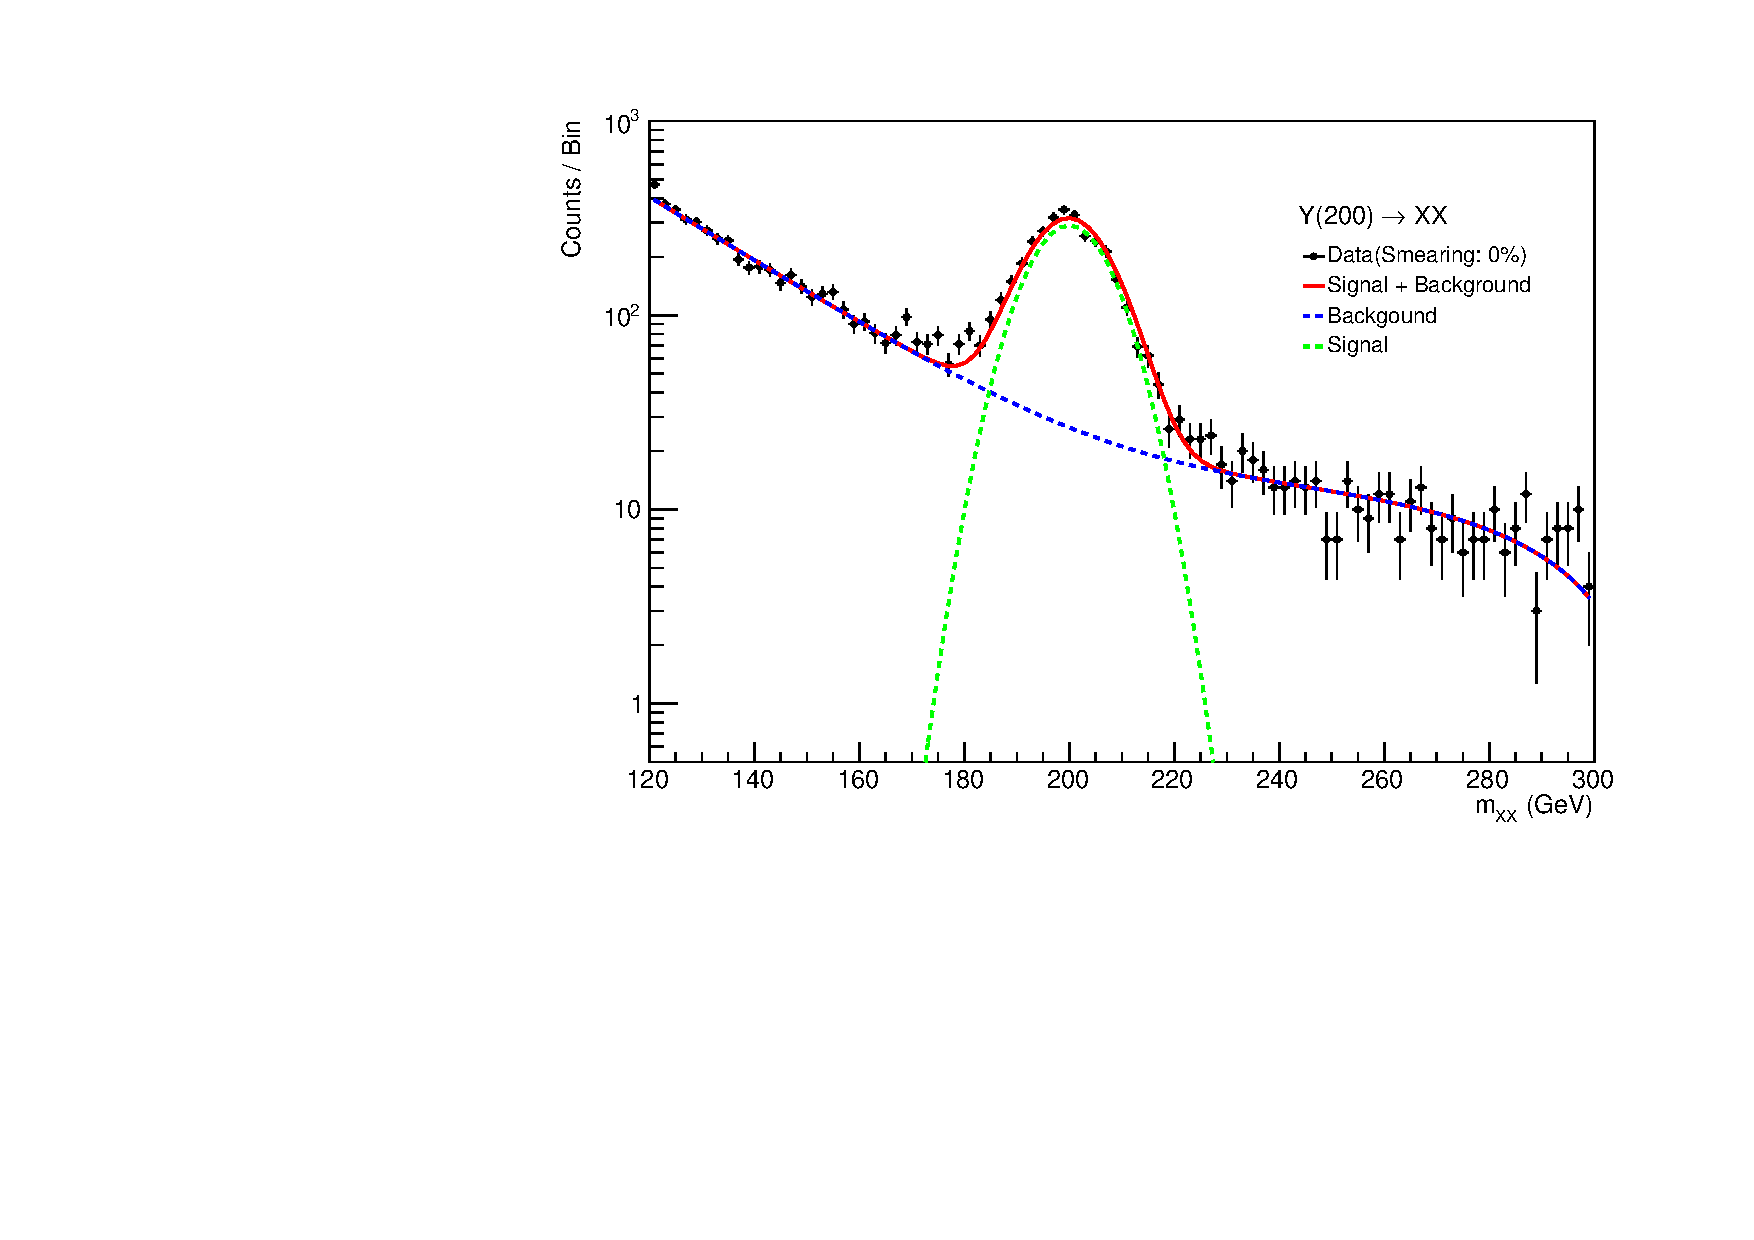
\includegraphics[page=1,width=\linewidth]{/home/kpapad/UG_thesis/Thesis/Analysis/src/WPhiJets_M200M100300_FitALL.pdf}
\caption{}
\end{subfigure}
\begin{subfigure}{0.45\textwidth}
\centering
\includegraphics[page=2,width=\linewidth]{/home/kpapad/UG_thesis/Thesis/Analysis/src/WPhiJets_M200M100300_FitALL.pdf}
\caption{}
\end{subfigure}

\begin{subfigure}{0.45\textwidth}
\centering
\includegraphics[page=3,width=\linewidth]{/home/kpapad/UG_thesis/Thesis/Analysis/src/WPhiJets_M200M100300_FitALL.pdf}
\caption{}
\end{subfigure}
\begin{subfigure}{0.45\textwidth}
\centering
\includegraphics[page=4,width=\linewidth]{/home/kpapad/UG_thesis/Thesis/Analysis/src/WPhiJets_M200M100300_FitALL.pdf}
\caption{}
\end{subfigure}

\begin{subfigure}{0.45\textwidth}
\centering
\includegraphics[page=5,width=\linewidth]{/home/kpapad/UG_thesis/Thesis/Analysis/src/WPhiJets_M200M100300_FitALL.pdf}
\caption{}
\end{subfigure}
\caption{Fits for the following smearing cases a: $0\%$, b:$5\%$, c:$10\%$, d:$15\%$, e:$20\%$}
\label{fig:fits}
\end{figure}

\begin{figure}[hbpt]
\centering
\begin{subfigure}{0.45\textwidth}
\centering
\includegraphics[page=6,width=\linewidth]{/home/kpapad/UG_thesis/Thesis/Analysis/src/WPhiJets_M200M100300_FitALL.pdf}
\caption{}
\end{subfigure}
\begin{subfigure}{0.45\textwidth}
\centering
\includegraphics[page=7,width=\linewidth]{/home/kpapad/UG_thesis/Thesis/Analysis/src/WPhiJets_M200M100300_FitALL.pdf}
\caption{}
\end{subfigure}

\begin{subfigure}{0.45\textwidth}
\centering
\includegraphics[page=8,width=\linewidth]{/home/kpapad/UG_thesis/Thesis/Analysis/src/WPhiJets_M200M100300_FitALL.pdf}
\caption{}
\end{subfigure}
\caption{Invariant mass spectra for the extreme smearing cases of : a:$30\%$, b:$40\%$ and c:$50\%$. The signal seems indistinguishable from the background in these cases, and therefore a fit based saparation cannot work.}
\label{fig:extremeSmearings}
\end{figure}

\newpage
\chapter{Search for light \(Y \rightarrow XX\)}
\label{sec:org59adc41}
\label{sec:Light_search_Y_to_XX}
\section{The light \(Y\rightarrow XX\) channel}
\label{sec:orgabd932d}
\label{Light_y_to_xx}
Similar to the previous study, the dataset used in the present analysis, is composed from a variety of pre-existing Monte Carlo (MC) samples, out of which only generator-level dileptonic final states are selected. The diobject invariant mass is in the range between 50 and 75 GeV, and no further kinematic constraints were placed in the event selection. Finally, the features of the set are summarized in Table \ref{table:DataSetFeatures}, and the invariant mass spectrum of the current decay is illustrated in figure \ref{fig:LightMassSpectrum}. It should be noted that in the study of such a generic process, there is no clear argument regarding a specific signal-to-background number of events ratio. Thus, the number of background and signal events is selected in a somewhat arbitrary manner, with the only condition being the minimization of statistical fluctuations.
\begin{figure}[h]
\centering
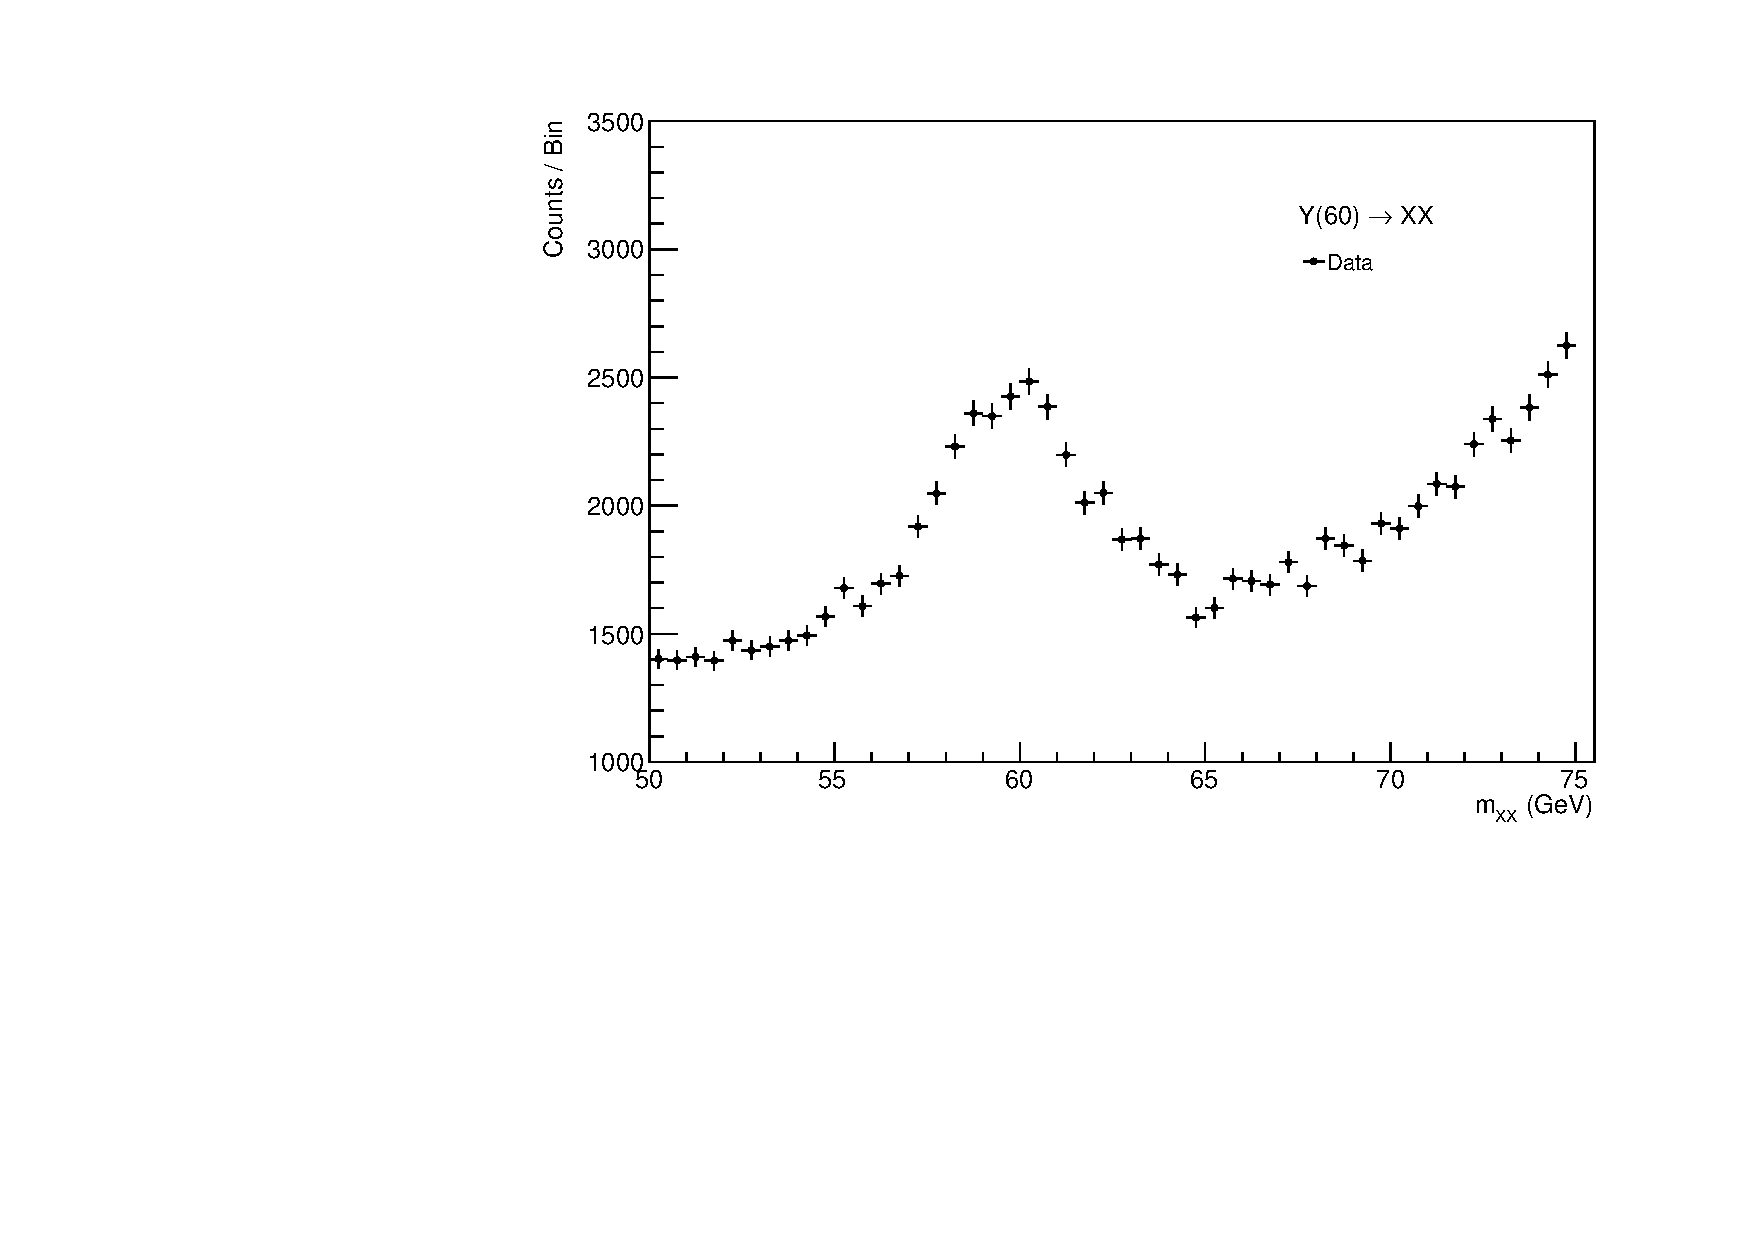
\includegraphics[width=0.5 \textwidth]{/home/kpapad/UG_thesis/Thesis/Analysis/out/Plots/DYJets_M60M5080_MassHist.pdf}
\caption{The $Y\rightarrow XX$ invariant mass spectrum}
\label{fig:LightMassSpectrum}
\end{figure}

\section{Energy scale uncertainties}
\label{sec:orga50049c}
\label{sec:Light_energy_scale_uncertainties}
The implementation of energy scale uncertainties in the present dataset is, once again, the same as in the heavy mass study presented in section \ref{sec:Energy_scale_uncertainties}, with the only difference being the percentage of smearing applied. For the particular invariant mass range, the available number of events is significantly lower, and therefore the effect of energy scale uncertainties on the mass is more significant. For that reason, we applied less smearing to the dataset, but nevertheless, we will study cases of mild and extreme smearing. Table \ref{table:LightSmearings} summarizes the cases that will be studied in the following sections.
\begin{table}[h!]
\centering
\begin{tabular}{ |c|  }
 \hline
Percentage of smearing \\
 \hline
$0\%$\\
$5\%$\\
$7\%$\\
$10\%$\\
$12\%$\\
\hline
\end{tabular}
\caption{Summary of the smearing cases that will be studied in the light mass search. }
\label{table:LightSmearings}
\end{table}
\section{Analysis method I: Training a BDT Classifier}
\label{sec:org6370180}
\subsection{The Train/Test/Application data sets}
\label{sec:org4e2ad68}
\label{sec:Light_train_test_application}
The number of training, testing, and application events is summarized in table \ref{table:LightTrainTestAppEvents}. Comparable to  section \ref{sec:Train_test_application_sets}, a part of the testing events was injected into the application set. However, due to a lack of extra signal, no additional events were used for the Training and Testing set.
\begin{table}[h!]
\centering
\begin{tabular}{ |p{3cm}|p{3cm}|p{4cm}|  }
 \hline
Data Set & No.Signal Events & No. Background Events \\
 \hline
Training & 3638 & 3638 \\
Testing & 3638 & 3638 \\
Application & 3638 & 29077 \\
 \hline
\end{tabular}
\caption{Sumarry of the Train Test Application number of events}
\label{table:LightTrainTestAppEvents}
\end{table}

\begin{figure}[h!]
\centering
\begin{subfigure}{0.49\textwidth}
\centering
\includegraphics[page=5, width=\linewidth]{/home/kpapad/UG_thesis/Thesis/Bdt/out/Plots/WPhiJets_M60M5080DeltasPConf13BDTplot.pdf}
\caption{}
\label{subfig:LightBdtPlot}
\end{subfigure}
\begin{subfigure}{0.49\textwidth}
\centering
\includegraphics[page=3, width=\linewidth]{/home/kpapad/UG_thesis/Thesis/Bdt/out/Plots/WPhiJets_M60M5080DeltasPConf12BDTplot.pdf}
\caption{}
\label{subfig:LightROCCurves}
\end{subfigure}
\caption{A: The BDT score of the Testing and Training sets. B: The roc curves for the training and testing sets}
\end{figure}

\newpage
\subsection{Training}
\label{sec:org02d5e1e}
\label{sec:LightTraining}
The feature space that results in the best model is still that of table \ref{table:TrainFeatures}. An illustration of the current features is shown in figure \ref{fig:LightFeatures}.
\begin{figure}[h!]
\centering
\includegraphics[page=1,width=\textwidth]{/home/kpapad/UG_thesis/Thesis/Analysis/out/Plots/WPhiJets_M60M5080DeltasVarsPlots.pdf}
\includegraphics[page=2,width=\textwidth]{/home/kpapad/UG_thesis/Thesis/Analysis/out/Plots/WPhiJets_M60M5080DeltasVarsPlots.pdf}
\caption{Sumarry of the features used for training }
\label{fig:LightFeatures}
\end{figure}

Figure \ref{subfig:LightBdtPlot} illustrates the BDT score of the trained model on the training and testing sets, while the corresponding ROC curves are shown in figure \ref{subfig:LightROCCurves}. The model's performance is assessed using the ROC curve and the AUC score. To evaluate overfitting, the ratio of the number of training events to the number of testing events at a particular BDT score is examined. Looking at figure \ref{subfig:LightBdtPlot}, the ratio of testing and training events fluctuates around one, indicating that the model is not severely overfit. Moreover, the AUC score that this model yields on the training events is 0.90, significantly lower than that of the model that was trained for the classification of the heavy mass dataset.

\subsection{Application}
\label{sec:orgf98812d}
\label{sec:Light_application}
The model's classification performance, on the classification sets, can be assessed by looking at figure \ref{fig:LightROCSIG}, which illustrates the ROC curves and the corresponding significances as a function of the BDT score, for the smearing cases of table \ref{table:LightSmearings}. It is evident that the model is not outstandingly affected by smearing, and thus, there is no point in selecting any other than the BDT score that yields the best significance. That is, placing the cut at BDT score = 0.96. The significance as a function of smearing, for the given cut can be seen in figure \ref{fig:LightSigEvolBDT}. Table \ref{table:LightNumSIGBKG} summarizes the amount of signal and background events present, for the selected cut.
\begin{figure}[h]
\centering
\begin{subfigure}{0.49\textwidth}
\centering
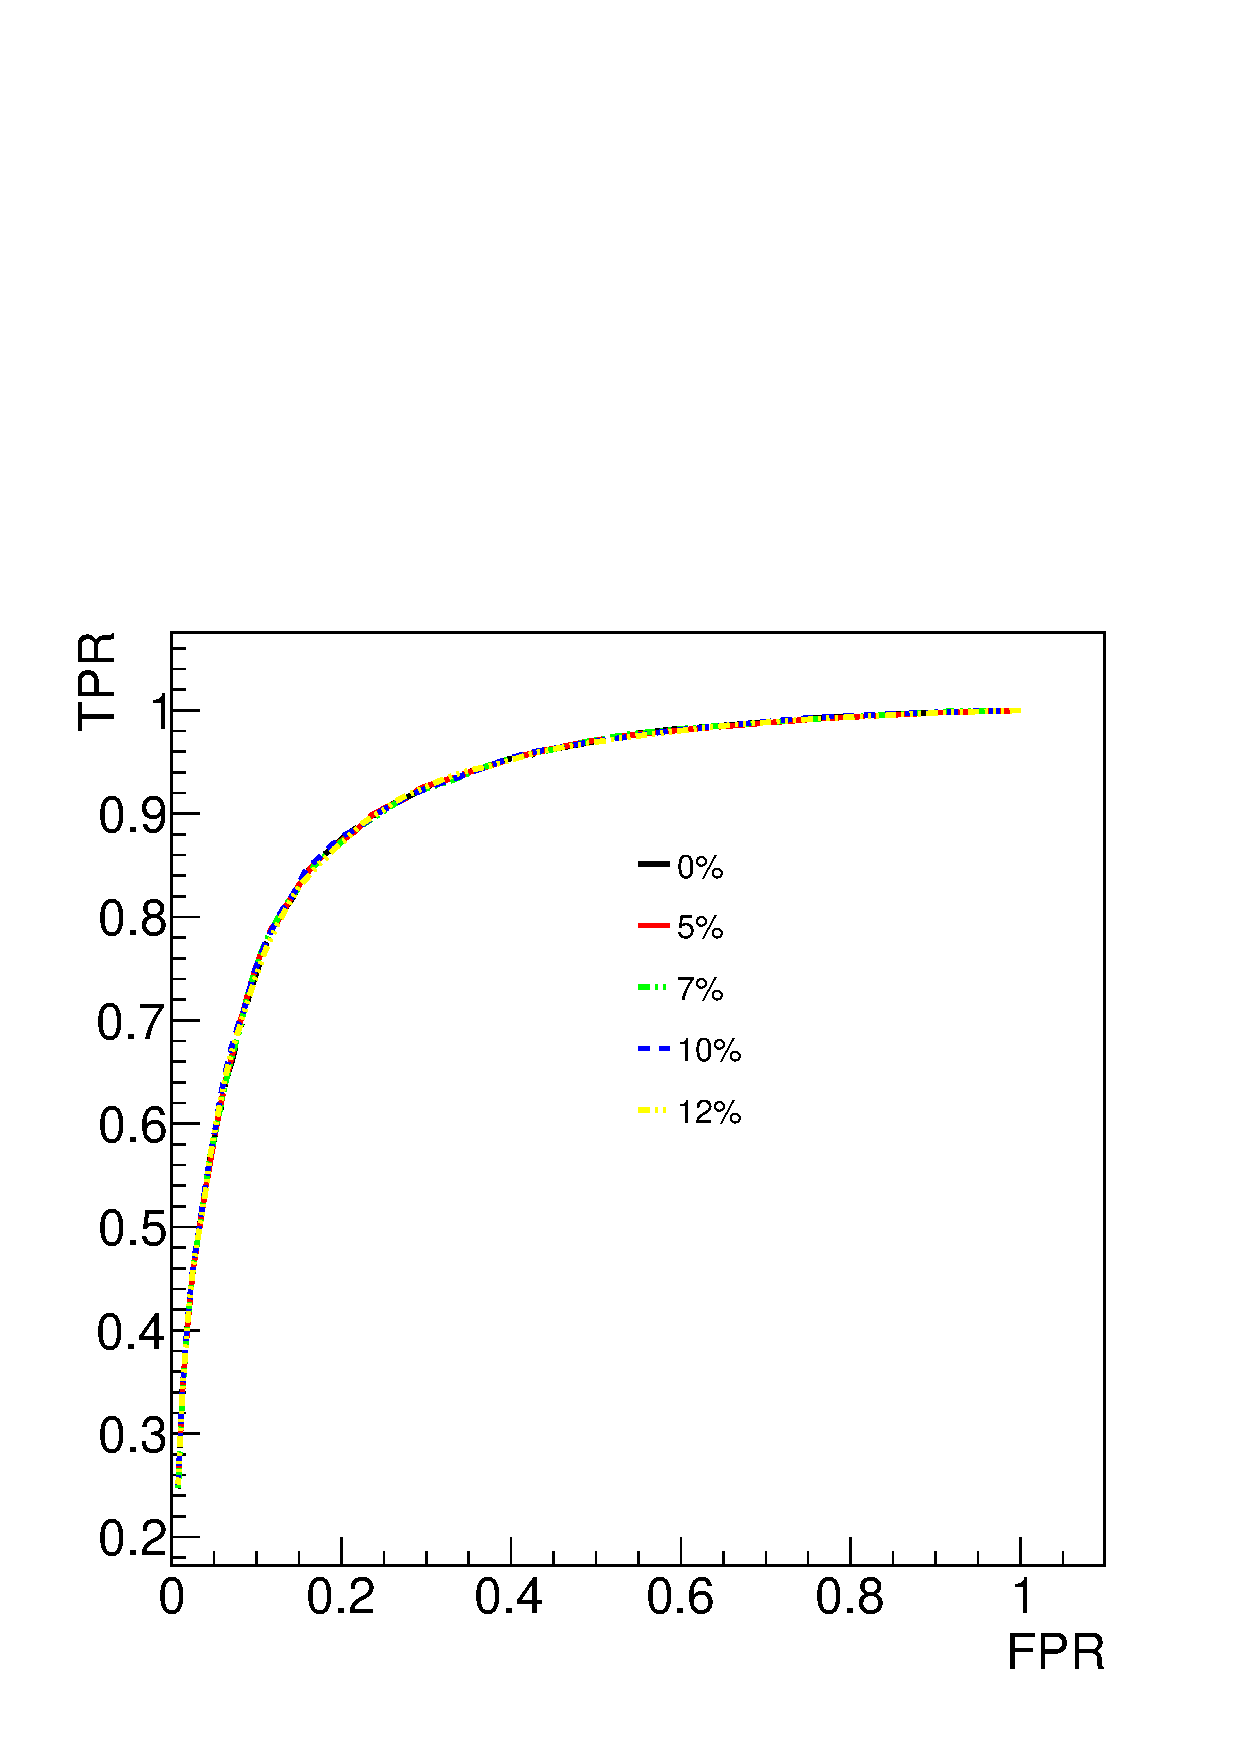
\includegraphics[page=1,width=\linewidth]{/home/kpapad/UG_thesis/Thesis/Bdt/src/WPhiJets_M60M5080_ROCs.pdf}
\caption{}
\end{subfigure}
\begin{subfigure}{0.49\textwidth}
\centering
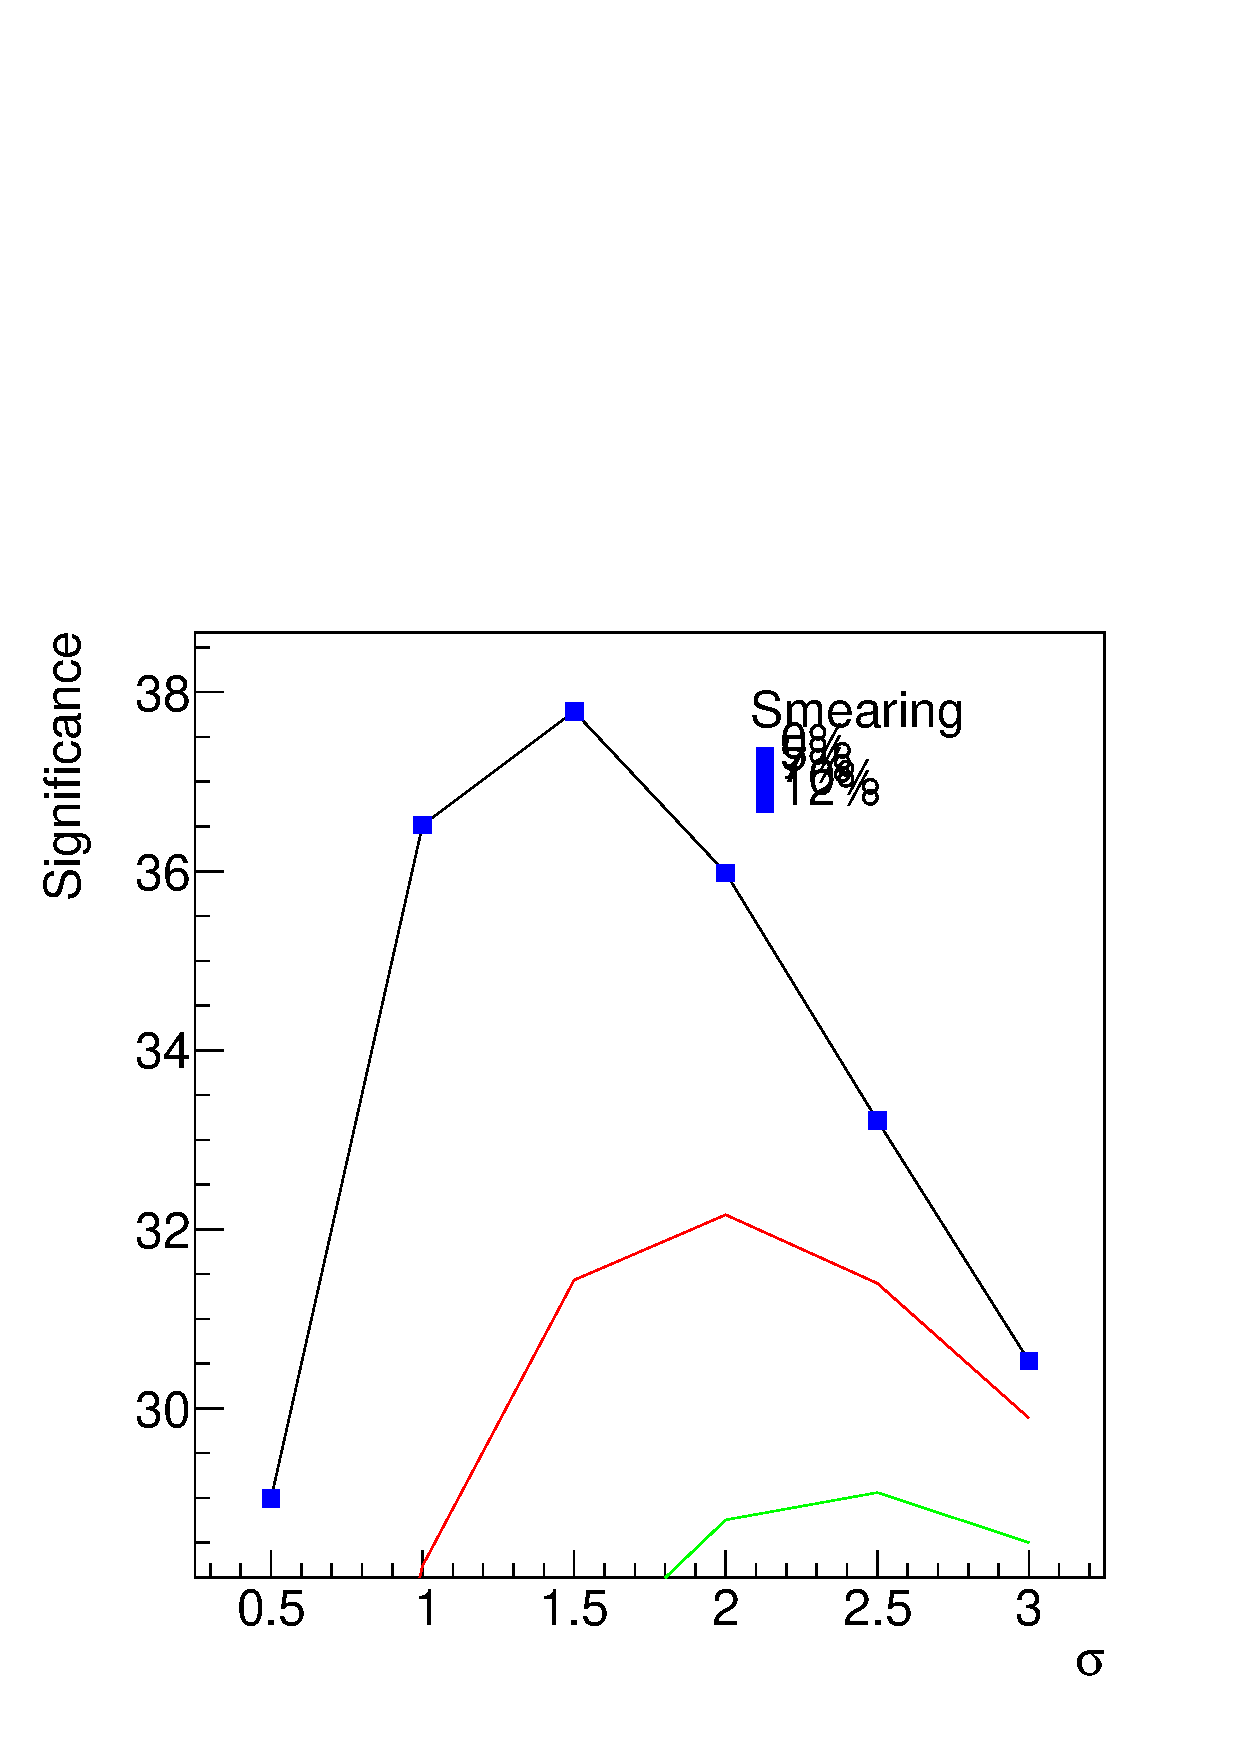
\includegraphics[page=1,width=\linewidth]{/home/kpapad/UG_thesis/Thesis/Bdt/src/WPhiJets_M60M5080_Significance.pdf}
\caption{}
\end{subfigure}
\caption{a: Summary of the ROC curves for the performance of the model on the data for each smearing case. b: Significances calculated across the BDT score range for the smearing cases of Table \ref{table:LightSmearings}. It is rather obvious that the perfomance of the classifier is the same for all the cases of smearing. }
\label{fig:LightROCSIG}
\end{figure}

\begin{table}[ht]
\centering
\begin{tabular}{|p{2cm}|p{3cm}|p{3cm}|}
 \hline
Smearing \%  & No. Sig. Events at BDT cut = 0.96 & No. Bkg.Events at BDT cut = 0.96 \\
\hline
0 & 1252 & 371 \\
5 & 912 & 371 \\
7 & 1235 & 371 \\
10 & 1246 & 371 \\
12 & 1243 & 371 \\
 \hline
\end{tabular}
\caption{Signal and background events at BDT cut 0.96 for different smearing percentages.}
\label{table:LightNumSIGBKG}
\end{table}

\begin{figure}[h!]
\centering
\includegraphics[page=2,width=0.5\textwidth]{/home/kpapad/UG_thesis/Thesis/Bdt/src/WPhiJets_M60M5080_Significance.pdf}
\caption{Evolution of significance for the smearing cases of table \ref{table:Smearings}. }
\label{fig:LightSigEvolBDT}
\end{figure}

\newpage
\section{Analysis Method II: Fit based analysis}
\label{sec:orgedb2280}
\label{sec:LightAnalysis_method2}
\subsection{Invariant mass reconstruction}
\label{sec:orgce79419}
\label{sec:Light_invariant_mass_reconstruction}
 The invariant mass spectrum is shown in Figure \ref{fig:LightAppMass}, and  is calculated using the features in Table \ref{table:DataSetFeatures}. 
\begin{figure}[h]
\centering
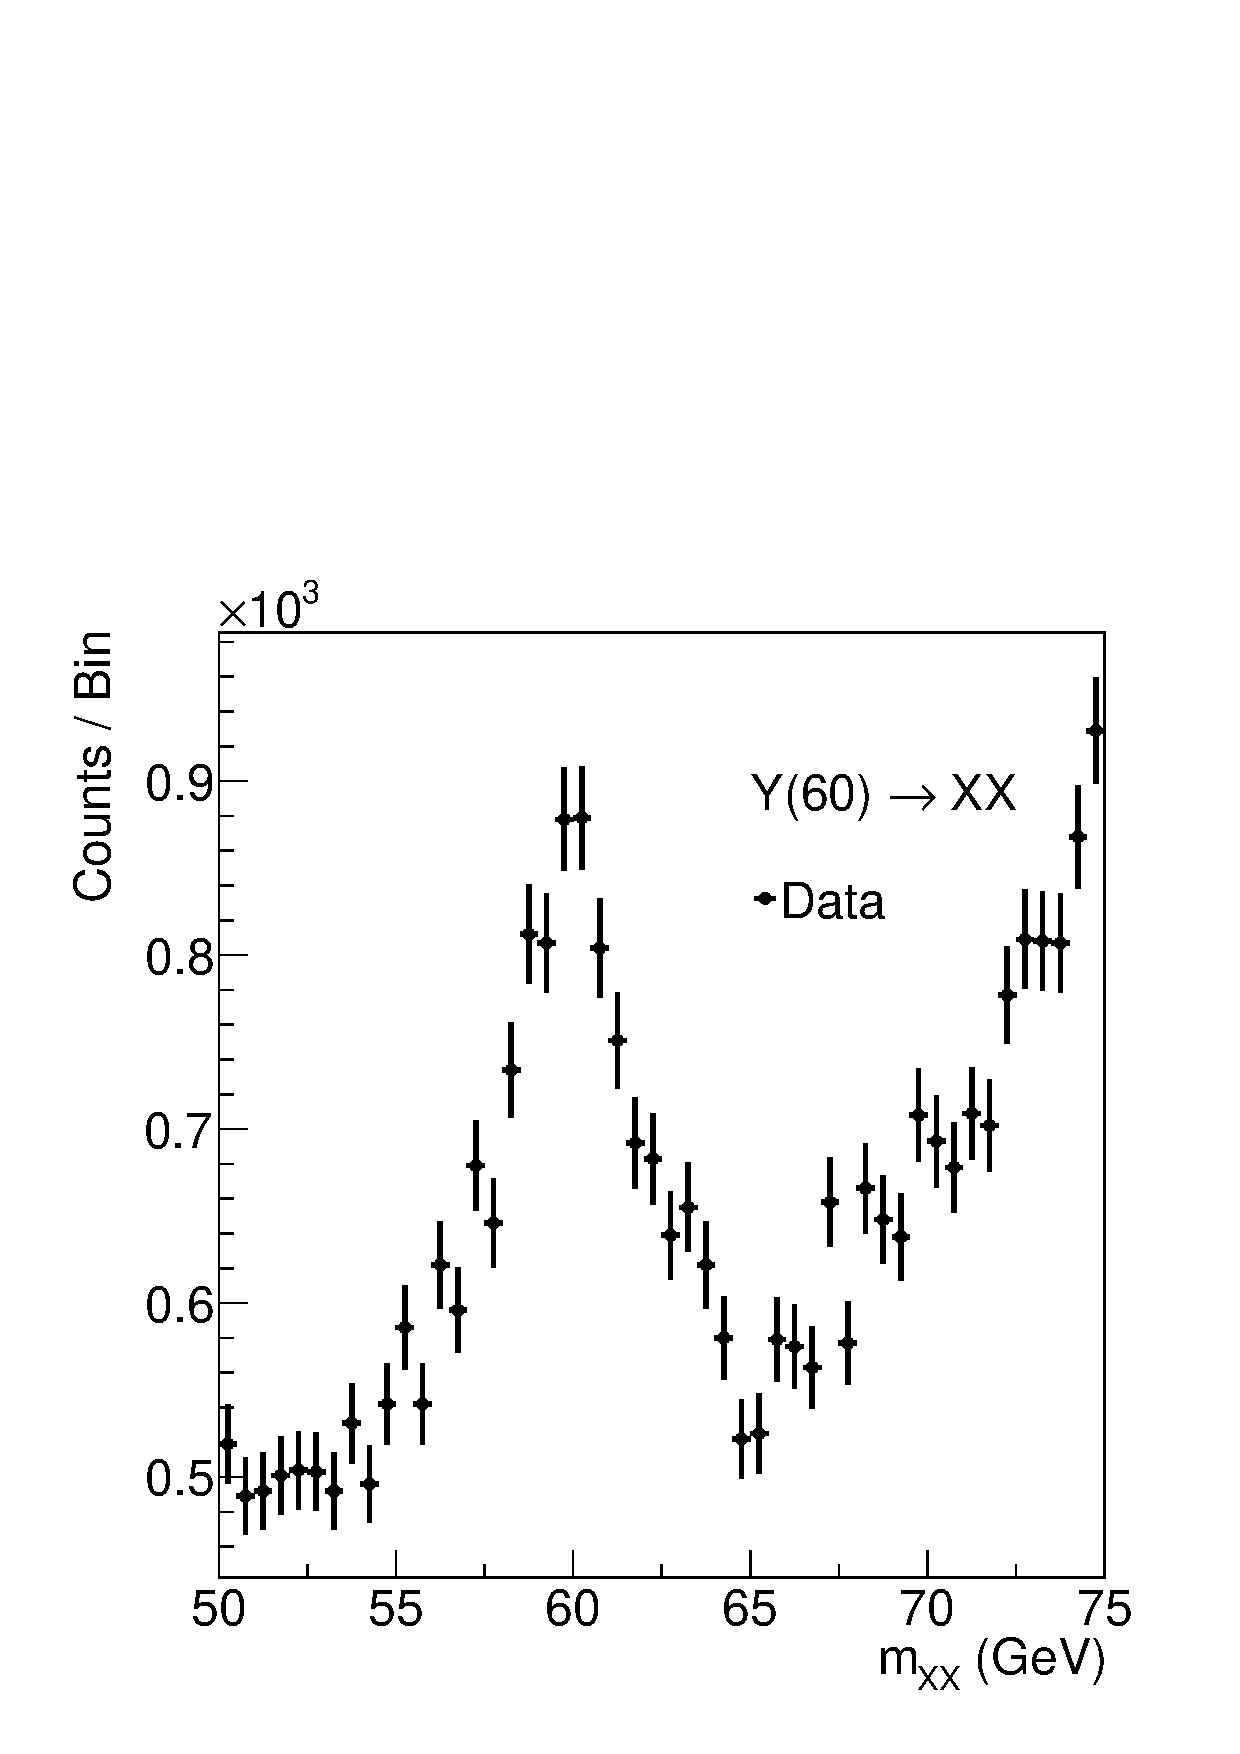
\includegraphics[page=1,width=0.5\textwidth]{/home/kpapad/UG_thesis/Thesis/Analysis/out/Plots/WPhiJets_M60M5080_Application_MassSpectrum.pdf}
\caption{The invariant mass spectrum of the application set}
\label{fig:LightAppMass}
\end{figure}

The reader may have noticed that the amount of signal present seems rather disproportionate to the amount of background. However, as discussed earlier, smearing has a significant effect on the present dataset due to low statistics. If it were not for the larger signal component, the invariant mass would have been completely smeared, even with very little smearing.
\subsection{Background Fitting}
\label{sec:orge8fa574}
\label{sec:Light_background_fitting}
We proceed with fitting the mass, using the simplification discussed in section \ref{sec:Background_fitting}. That is, the background shape is fitted separately and kept constant throughout the signal fits.

The background shape is described by the function shown in Equation \ref{eq:LightbkgFitFunc}.
\begin{equation}
bkg(x) =  \alpha + \beta x + \gamma x^2 + \delta x^3,
\label{eq:LightbkgFitFunc}
\end{equation}
The parameters \(\alpha\), \(\beta\), \(\gamma\), and \(\delta\) are free parameters of the fit. The modeled background is illustrated in Figure \ref{fig:LightBKGfit}.
\begin{figure}[h]
\centering
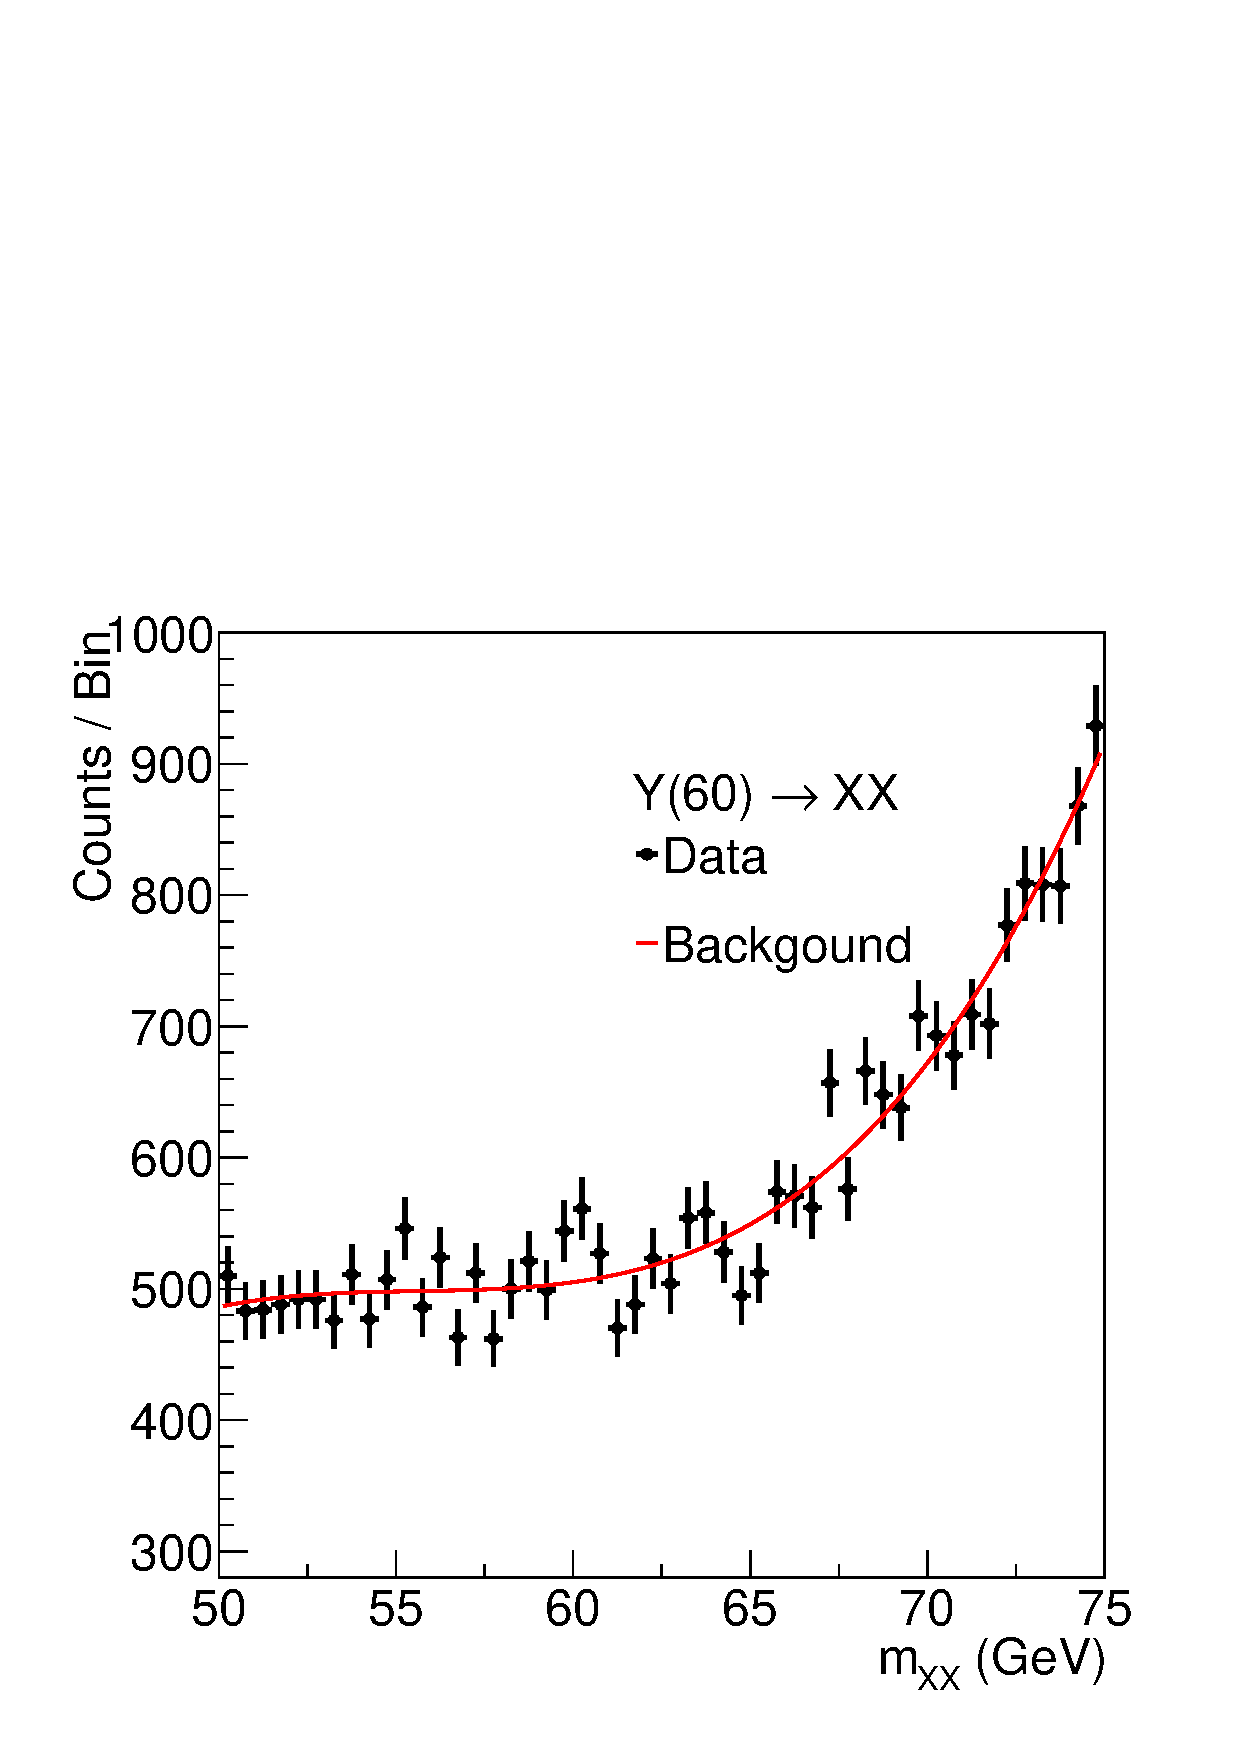
\includegraphics[page=1,width=0.5\textwidth]{/home/kpapad/UG_thesis/Thesis/Analysis/out/Plots/WPhiJets_M60M5080_Application_bkgonly_Fit.pdf}
\caption{The fitted background}
\label{fig:LightBKGfit}
\end{figure}
\subsection{Signal Fitting}
\label{sec:orgd9ebfef}
\label{sec:Light_signal_fitting}
To fit the signal, a Gaussian function with \(\sigma\) and magnitude as free parameters, and \(\mu = 60\text{GeV}\), is used. Figure \ref{fig:Lightfits} shows the fitted invariant mass spectra for smearing percentages of \(0\%\), \(5\%\), \(7\%\), \(10\%\), and \(12\%\). As shown in Figure \ref{fig:Lightfits}, smearing cases above \(12\%\) would completely smear the signal component, and the fit analysis method would have failed.
\subsection{Signal from background separation}
\label{sec:orgb4ae30e}
\label{sec:Light_signal_from_background_separation}
The signal from the background separation process in this study is the same as that in section \ref{sec:Signal_from_background_separation}. We scan various mass windows around the center of the signal to find the region that yields the best significance. Moving with a step of \(0.5\sigma\), we scanned six different regions from \(\pm 0.5\sigma\) up to \(\pm 3\sigma\). Looking at the results in figure \ref{subfig:LightScan0}, the region \(\pm 1.5\sigma\) provides the best performance in terms of significance.
\begin{figure}[h]
\centering
\begin{subfigure}{0.45\textwidth}
\centering
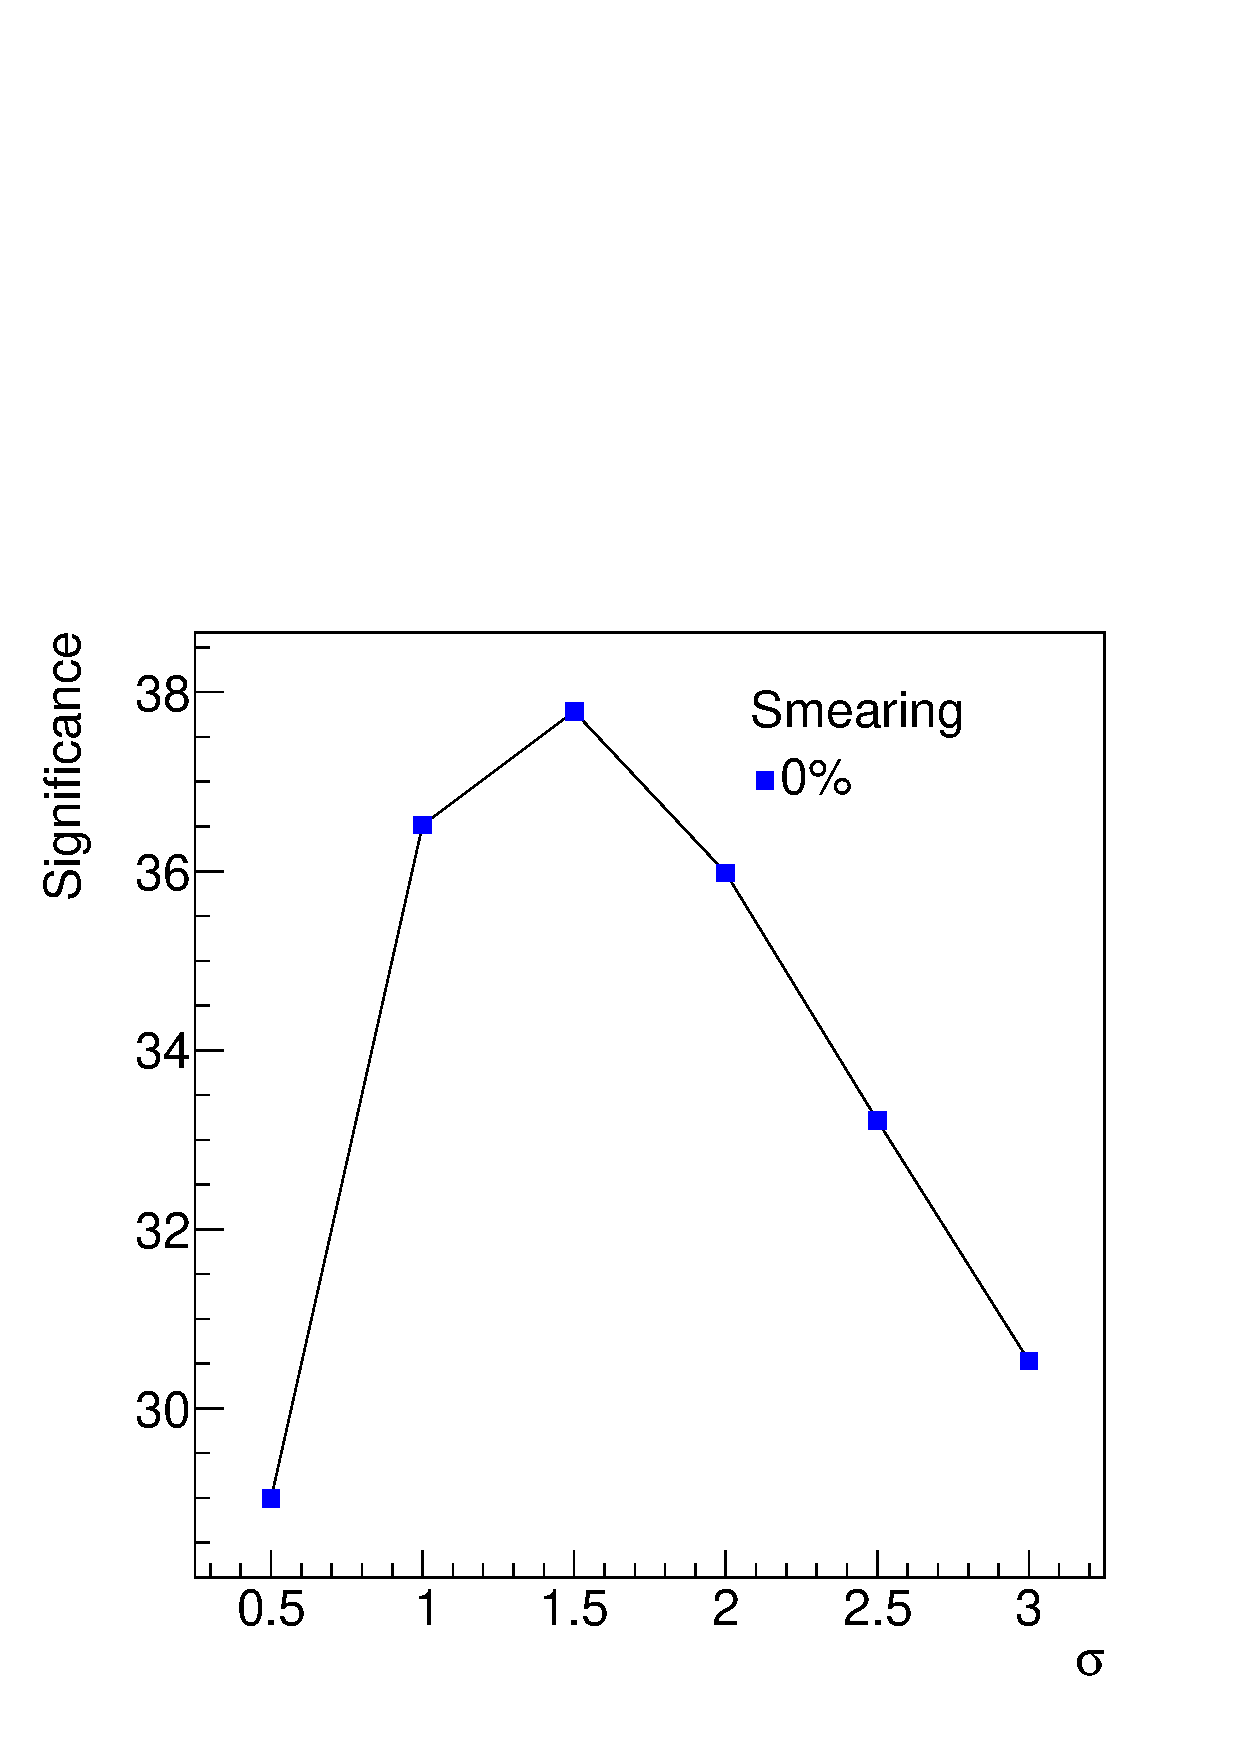
\includegraphics[page=1,width=\linewidth]{/home/kpapad/UG_thesis/Thesis/Analysis/src/WPhiJets_M60M5080_Significance0.pdf}
\caption{}
\label{subfig:LightScan0}
\end{subfigure}
\begin{subfigure}{0.45\textwidth}
\centering
\includegraphics[page=3,width=\linewidth]{/home/kpapad/UG_thesis/Thesis/Bdt/src/WPhiJets_M60M5080_Significance.pdf}
\caption{}
\label{subfig:LightAdaFixedSig}
\end{subfigure}
\caption{a: Scan of significance for various values of $\sigma$, in the $0\%$ smearing case. We see that the regrion $\pm 1.5\sigma$ around $\mu=60GeV$, gives the best significance, b: Copmarison of the significance evolution as caclulated in the fixed widow and adaptive window case.}
\end{figure}

We study the changes in significance as a function of smearing, in the fixed window and adaptive window interpretations discussed in section \ref{sec:Signal_from_background_separation}. The actual values of \(\sigma\), and the corresponding mass window for the adaptive window search, are summarized in table \ref{table:LightAdaSigmas}. The results are presented in Figure \ref{subfig:LightAdaFixedSig}, and Table \ref{table:LightNumSigBkg}, which summarizes the amount of signal and background events present in the region of interest for both studies (fixed and adaptive window).
\begin{table}[h]
\centering
\begin{tabular}{|p{2cm}|p{2cm}|c|}
 \hline
Smearing \%  & $\sigma$ in GeV & Invarian Mass $\pm 1.5\sigma$ window  in GeV \\
\hline
0 & 2.1267 & 6.38 \\
5 & 2.9933 & 8.98 \\
7 & 3.6933 & 11.08 \\
10 & 4.84 & 14.52 \\
12 & 5.5133 & 16.54 \\
 \hline
\end{tabular}
\caption{Summary of the invariant mass windows used used in adapitve window study. Note that the resulting window of $0\%$ smearing corresponds to the fixed window case as well.}
\label{table:LightAdaSigmas}
\end{table}

\begin{table}[h!]
\centering
\begin{tabular}{|p{2cm}|p{3cm}|p{3cm}|p{3cm}|p{3cm}|}
 \hline
Smearing \%  & No. Sig. Events (fixed window) & No. Bkg.Events (fixed window) & No. Sig. Events (adaptive window) & No. Bkg.Events (adaptive window)  \\
\hline
0 & 3040 & 6474 & 3040 & 6474 \\
5 & 2529 & 6474 & 3069 & 9150 \\
7 & 2183 & 6474 & 3091 & 11364 \\
10 & 1770 & 6474 & 3131 & 15049 \\
12 & 1553 & 6474 & 3080 & 17263 \\
 \hline
\end{tabular}
\caption{Signal and background events in the 6.38Gev fixed window region and in the $\pm 1.5\sigma$ adaptive window region, for different smearing percentages.}
\label{table:LightNumSigBkg}
\end{table}

\newpage
\section{Results}
\label{sec:org7065c84}
The study of multivariate and single variate classification techniques in a signal from background separation task, in the lower mass region, returned interesting results, which are going to be discussed in the present section. 
\begin{figure}[h]
\centering
\includegraphics[page=4,width=0.5\textwidth]{/home/kpapad/UG_thesis/Thesis/Bdt/src/WPhiJets_M60M5080_Significance.pdf}
\caption{ Comparison of the perfomance of the BDT and Fit based analysis, in terms of sifnificance,  as a function of the smearing cases. We can see that BDT based analysis, is more robust.}
\label{fig:LightBdtFitSig}
\end{figure}

A comparison between the significance yielded by each method, as a function of smearing, is presented in Figure \ref{fig:LightBdtFitSig}. What is striking is the performance, in terms of significance, of the two methods. It is evident that the BDT classifier provides the best performance, while being more or less unaffected by energy scale uncertainties. To further investigate this compelling result, we can take a look at the model's feature importance (a score that indicates how useful or valuable each feature was in the construction of the boosted decision trees within the model), presented in Figure \ref{fig:LightFeatureImportance}. Even though the actual meaning of the score is different depending on the training algorithm, the feature whose role is the most significant in the classification task, is the \(\Delta\phi\) of the particles, a variable that as already mentioned, is not affected by smearing.

On the other hand, the performance of the fit model is similar to that of the heavy mass search. The significance it returns drops as the invariant mass smearing percentage increases, until it reaches a "breaking point".
\begin{figure}[h!]
\centering
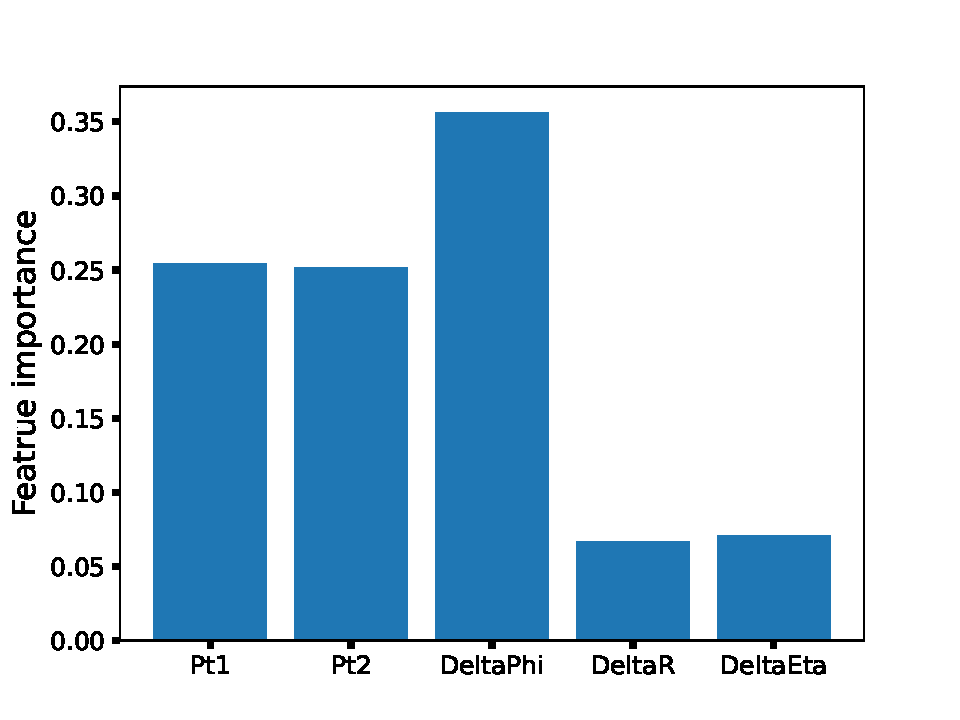
\includegraphics[page=1,width=0.5\textwidth]{/home/kpapad/UG_thesis/Thesis/Bdt/out/Plots/feature_importance_lm.pdf}
\caption{The feature importance of the BDT classifier. The model's performance on smeared data is rather stable, due to its strong dependance on $\Delta\phi$, a variable that remains invariant under smearing. }
\label{fig:LightFeatureImportance}
\end{figure}

\begin{figure}[htbp]
\centering
\begin{subfigure}{0.45\textwidth}
\centering
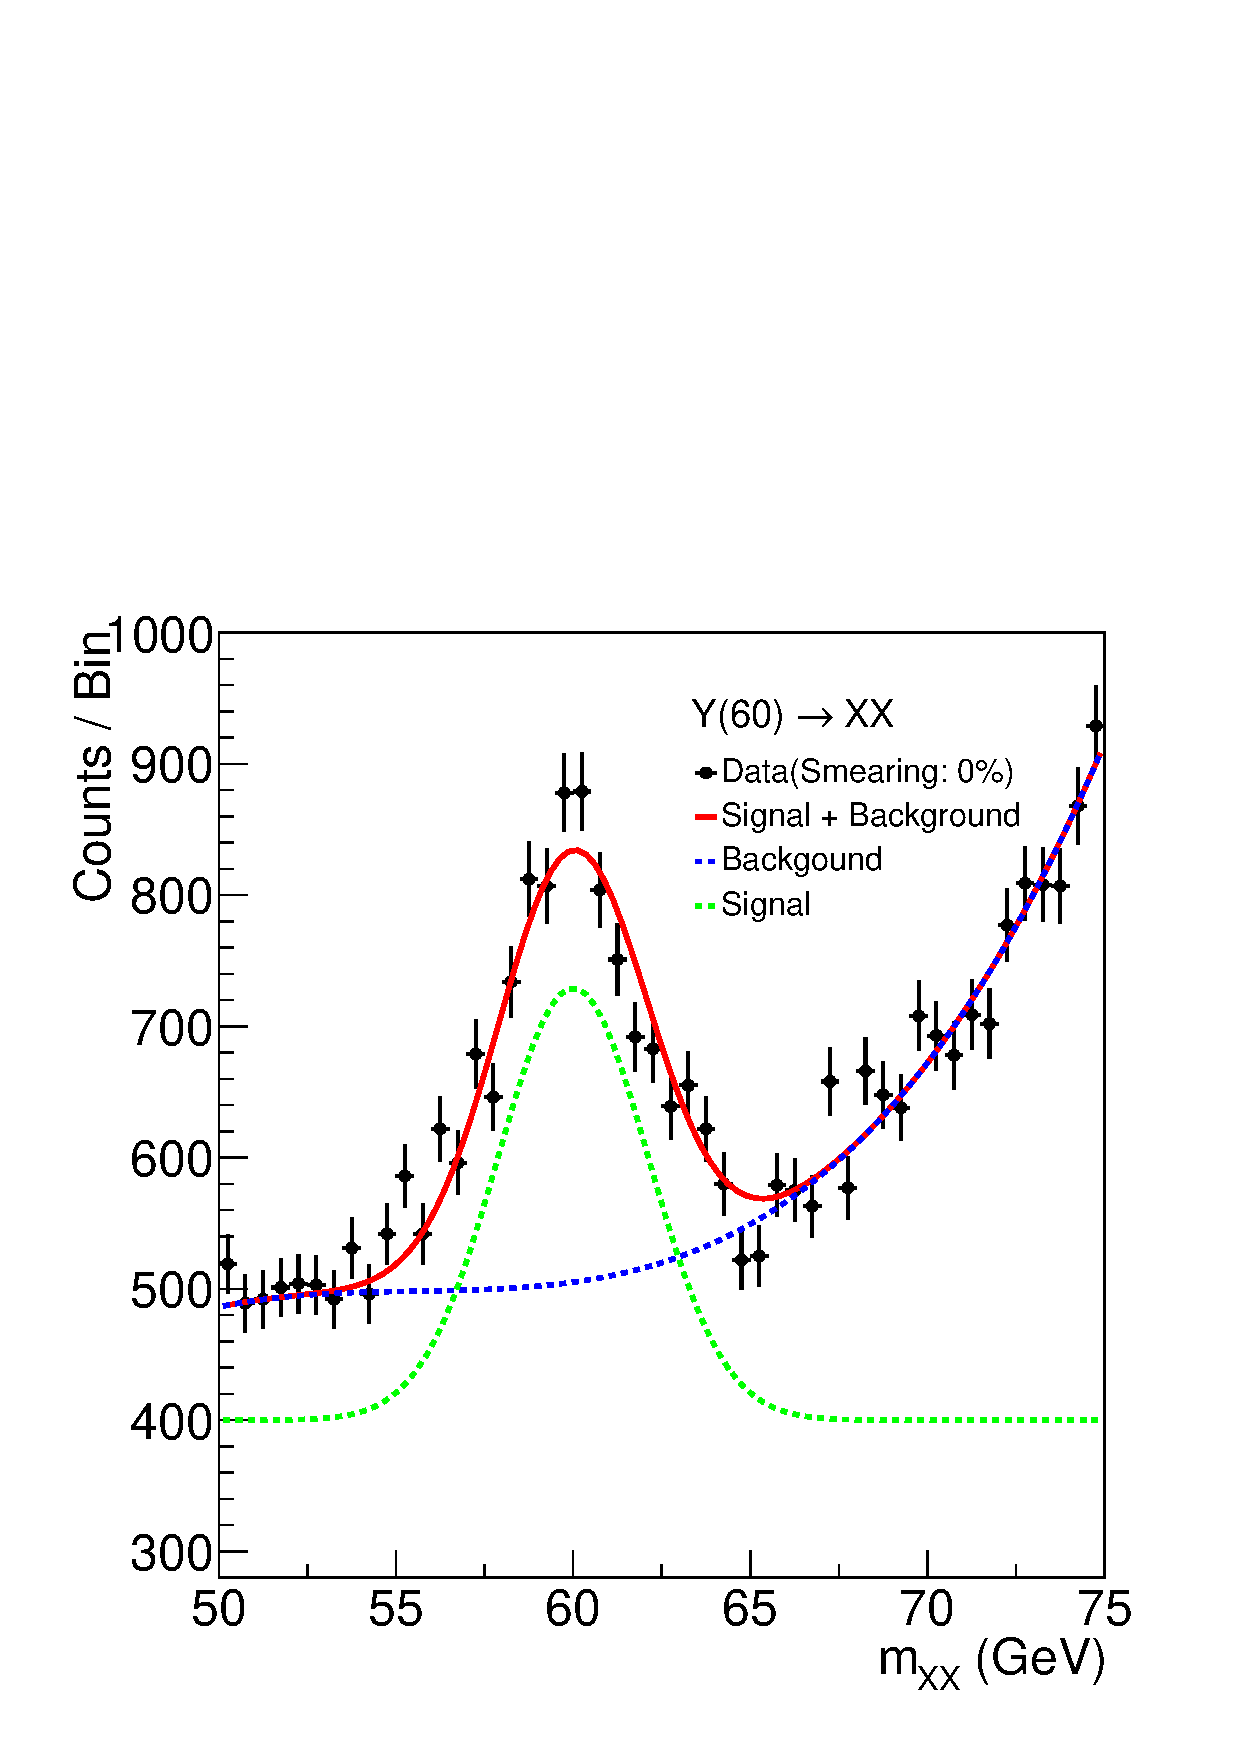
\includegraphics[page=1,width=\linewidth]{/home/kpapad/UG_thesis/Thesis/Analysis/src/WPhiJets_M60M5080_FitALL.pdf}
\caption{}
\end{subfigure}
\begin{subfigure}{0.45\textwidth}
\centering
\includegraphics[page=2,width=\linewidth]{/home/kpapad/UG_thesis/Thesis/Analysis/src/WPhiJets_M60M5080_FitALL.pdf}
\caption{}
\end{subfigure}

\begin{subfigure}{0.45\textwidth}
\centering
\includegraphics[page=3,width=\linewidth]{/home/kpapad/UG_thesis/Thesis/Analysis/src/WPhiJets_M60M5080_FitALL.pdf}
\caption{}
\end{subfigure}
\begin{subfigure}{0.45\textwidth}
\centering
\includegraphics[page=4,width=\linewidth]{/home/kpapad/UG_thesis/Thesis/Analysis/src/WPhiJets_M60M5080_FitALL.pdf}
\caption{}
\end{subfigure}

\begin{subfigure}{0.45\textwidth}
\centering
\includegraphics[page=5,width=\linewidth]{/home/kpapad/UG_thesis/Thesis/Analysis/src/WPhiJets_M60M5080_FitALL.pdf}
\caption{}
\end{subfigure}
\caption{Fits for the following smearing cases a: $0\%$, b: $5\%$, c: $7\%$, d: $10\%$, e: $12\%$}
\label{fig:Lightfits}
\end{figure}

\clearpage
\section{Conclusion}
\label{sec:org11ceed0}
In this work, we present a study of the interplay between multivariate and single variate classification techniques, and energy scale uncertainties in the search for both heavy and light diobject resonances at the LHC. Moreover, we consider a plethora of cases of uncertainties in the energy scale, in the analysis of the performance of a BDT model, and a fit-based analysis.

Overall, we observe that the BDT model is more robust when systematic uncertainties are present, while delivering better performance in terms of significance. Such behavior is related to the fact that the classifier learns (in a rather unphysical way) to classify the signal and background using features that are not affected by energy scale uncertainties.

This does not mean that a fit-based analysis is of no use, as there are ways to enhance its performance. Specifically, looking at the feature space discussed in Sections \ref{sec:Training} and \ref{sec:LightTraining}, it is rather evident that the feature that helps the most with the distinction between the signal and background, while being invariant to energy scale uncertainties, is the azimuthal angle difference of the two produced Xs. Therefore, with a more careful event selection, one can reject a significant portion of the background by taking into consideration the \(\Delta \phi\) of the pair, which is expected to result in a better performance of the fit-based approach.

Nevertheless, through the thorough analysis presented in this thesis, we conclude that when systematic uncertainties are introduced to the problem, there will be cases where the signal mass will be smeared away completely, making the use of univariate classification techniques challenging. In such cases, it is expected that a multivariate classification method, like a BDT model, will be able to perform the task and deliver decent performance.

Finally, to train the BDT model, we had to find the feature space that exploits the differences between signal and background in the most efficient way. In our case, the best features were the Pt of the particles, \(\Delta\Phi\), \(\Delta\eta\) and \(\Delta R\). As discussed, the most helpful geometric feature for the distinction of the particles is the difference in the azimuthal angle of the pair. This difference in \(\Delta \phi\) is inherited from the MC samples we used for the signal and background (background comes from the Drell-Yan process, and signal from W\(\Phi\) to ll), be that as it may, the argument that the resulting dataset can be treated as a generic diobject production still holds. For if the parent MC samples were different, the best features would also have been different, but the rest of the analysis would have been the same, a process-agnostic search.


%% Chapter 1

\chapter{Chapter Title Here} % Main chapter title

\label{Chapter1} % For referencing the chapter elsewhere, use \ref{Chapter1} 

%----------------------------------------------------------------------------------------

% Define some commands to keep the formatting separated from the content 
\newcommand{\keyword}[1]{\textbf{#1}}
\newcommand{\tabhead}[1]{\textbf{#1}}
\newcommand{\code}[1]{\texttt{#1}}
\newcommand{\file}[1]{\texttt{\bfseries#1}}
\newcommand{\option}[1]{\texttt{\itshape#1}}

%----------------------------------------------------------------------------------------

\section{Welcome and Thank You}
Welcome to this \LaTeX{} Thesis Template, a beautiful and easy to use template for writing a thesis using the \LaTeX{} typesetting system.

If you are writing a thesis (or will be in the future) and its subject is technical or mathematical (though it doesn't have to be), then creating it in \LaTeX{} is highly recommended as a way to make sure you can just get down to the essential writing without having to worry over formatting or wasting time arguing with your word processor.

\LaTeX{} is easily able to professionally typeset documents that run to hundreds or thousands of pages long. With simple mark-up commands, it automatically sets out the table of contents, margins, page headers and footers and keeps the formatting consistent and beautiful. One of its main strengths is the way it can easily typeset mathematics, even \emph{heavy} mathematics. Even if those equations are the most horribly twisted and most difficult mathematical problems that can only be solved on a super-computer, you can at least count on \LaTeX{} to make them look stunning.

%----------------------------------------------------------------------------------------

\section{Learning \LaTeX{}}

\LaTeX{} is not a \textsc{wysiwyg} (What You See is What You Get) program, unlike word processors such as Microsoft Word or Apple's Pages. Instead, a document written for \LaTeX{} is actually a simple, plain text file that contains \emph{no formatting}. You tell \LaTeX{} how you want the formatting in the finished document by writing in simple commands amongst the text, for example, if I want to use \emph{italic text for emphasis}, I write the \verb|\emph{text}| command and put the text I want in italics in between the curly braces. This means that \LaTeX{} is a \enquote{mark-up} language, very much like HTML.

\subsection{A (not so short) Introduction to \LaTeX{}}

If you are new to \LaTeX{}, there is a very good eBook -- freely available online as a PDF file -- called, \enquote{The Not So Short Introduction to \LaTeX{}}. The book's title is typically shortened to just \emph{lshort}. You can download the latest version (as it is occasionally updated) from here:
\url{http://www.ctan.org/tex-archive/info/lshort/english/lshort.pdf}

It is also available in several other languages. Find yours from the list on this page: \url{http://www.ctan.org/tex-archive/info/lshort/}

It is recommended to take a little time out to learn how to use \LaTeX{} by creating several, small `test' documents, or having a close look at several templates on:\\ 
\url{http://www.LaTeXTemplates.com}\\ 
Making the effort now means you're not stuck learning the system when what you \emph{really} need to be doing is writing your thesis.

\subsection{A Short Math Guide for \LaTeX{}}

If you are writing a technical or mathematical thesis, then you may want to read the document by the AMS (American Mathematical Society) called, \enquote{A Short Math Guide for \LaTeX{}}. It can be found online here:
\url{http://www.ams.org/tex/amslatex.html}
under the \enquote{Additional Documentation} section towards the bottom of the page.

\subsection{Common \LaTeX{} Math Symbols}
There are a multitude of mathematical symbols available for \LaTeX{} and it would take a great effort to learn the commands for them all. The most common ones you are likely to use are shown on this page:
\url{http://www.sunilpatel.co.uk/latex-type/latex-math-symbols/}

You can use this page as a reference or crib sheet, the symbols are rendered as large, high quality images so you can quickly find the \LaTeX{} command for the symbol you need.

\subsection{\LaTeX{} on a Mac}
 
The \LaTeX{} distribution is available for many systems including Windows, Linux and Mac OS X. The package for OS X is called MacTeX and it contains all the applications you need -- bundled together and pre-customized -- for a fully working \LaTeX{} environment and work flow.
 
MacTeX includes a custom dedicated \LaTeX{} editor called TeXShop for writing your `\file{.tex}' files and BibDesk: a program to manage your references and create your bibliography section just as easily as managing songs and creating playlists in iTunes.

%----------------------------------------------------------------------------------------

\section{Getting Started with this Template}

If you are familiar with \LaTeX{}, then you should explore the directory structure of the template and then proceed to place your own information into the \emph{THESIS INFORMATION} block of the \file{main.tex} file. You can then modify the rest of this file to your unique specifications based on your degree/university. Section \ref{FillingFile} on page \pageref{FillingFile} will help you do this. Make sure you also read section \ref{ThesisConventions} about thesis conventions to get the most out of this template.

If you are new to \LaTeX{} it is recommended that you carry on reading through the rest of the information in this document.

Before you begin using this template you should ensure that its style complies with the thesis style guidelines imposed by your institution. In most cases this template style and layout will be suitable. If it is not, it may only require a small change to bring the template in line with your institution's recommendations. These modifications will need to be done on the \file{MastersDoctoralThesis.cls} file.

\subsection{About this Template}

This \LaTeX{} Thesis Template is originally based and created around a \LaTeX{} style file created by Steve R.\ Gunn from the University of Southampton (UK), department of Electronics and Computer Science. You can find his original thesis style file at his site, here:
\url{http://www.ecs.soton.ac.uk/~srg/softwaretools/document/templates/}

Steve's \file{ecsthesis.cls} was then taken by Sunil Patel who modified it by creating a skeleton framework and folder structure to place the thesis files in. The resulting template can be found on Sunil's site here:
\url{http://www.sunilpatel.co.uk/thesis-template}

Sunil's template was made available through \url{http://www.LaTeXTemplates.com} where it was modified many times based on user requests and questions. Version 2.0 and onwards of this template represents a major modification to Sunil's template and is, in fact, hardly recognisable. The work to make version 2.0 possible was carried out by \href{mailto:vel@latextemplates.com}{Vel} and Johannes Böttcher.

%----------------------------------------------------------------------------------------

\section{What this Template Includes}

\subsection{Folders}

This template comes as a single zip file that expands out to several files and folders. The folder names are mostly self-explanatory:

\keyword{Appendices} -- this is the folder where you put the appendices. Each appendix should go into its own separate \file{.tex} file. An example and template are included in the directory.

\keyword{Chapters} -- this is the folder where you put the thesis chapters. A thesis usually has about six chapters, though there is no hard rule on this. Each chapter should go in its own separate \file{.tex} file and they can be split as:
\begin{itemize}
\item Chapter 1: Introduction to the thesis topic
\item Chapter 2: Background information and theory
\item Chapter 3: (Laboratory) experimental setup
\item Chapter 4: Details of experiment 1
\item Chapter 5: Details of experiment 2
\item Chapter 6: Discussion of the experimental results
\item Chapter 7: Conclusion and future directions
\end{itemize}
This chapter layout is specialised for the experimental sciences, your discipline may be different.

\keyword{Figures} -- this folder contains all figures for the thesis. These are the final images that will go into the thesis document.

\subsection{Files}

Included are also several files, most of them are plain text and you can see their contents in a text editor. After initial compilation, you will see that more auxiliary files are created by \LaTeX{} or BibTeX and which you don't need to delete or worry about:

\keyword{example.bib} -- this is an important file that contains all the bibliographic information and references that you will be citing in the thesis for use with BibTeX. You can write it manually, but there are reference manager programs available that will create and manage it for you. Bibliographies in \LaTeX{} are a large subject and you may need to read about BibTeX before starting with this. Many modern reference managers will allow you to export your references in BibTeX format which greatly eases the amount of work you have to do.

\keyword{MastersDoctoralThesis.cls} -- this is an important file. It is the class file that tells \LaTeX{} how to format the thesis. 

\keyword{main.pdf} -- this is your beautifully typeset thesis (in the PDF file format) created by \LaTeX{}. It is supplied in the PDF with the template and after you compile the template you should get an identical version.

\keyword{main.tex} -- this is an important file. This is the file that you tell \LaTeX{} to compile to produce your thesis as a PDF file. It contains the framework and constructs that tell \LaTeX{} how to layout the thesis. It is heavily commented so you can read exactly what each line of code does and why it is there. After you put your own information into the \emph{THESIS INFORMATION} block -- you have now started your thesis!

Files that are \emph{not} included, but are created by \LaTeX{} as auxiliary files include:

\keyword{main.aux} -- this is an auxiliary file generated by \LaTeX{}, if it is deleted \LaTeX{} simply regenerates it when you run the main \file{.tex} file.

\keyword{main.bbl} -- this is an auxiliary file generated by BibTeX, if it is deleted, BibTeX simply regenerates it when you run the \file{main.aux} file. Whereas the \file{.bib} file contains all the references you have, this \file{.bbl} file contains the references you have actually cited in the thesis and is used to build the bibliography section of the thesis.

\keyword{main.blg} -- this is an auxiliary file generated by BibTeX, if it is deleted BibTeX simply regenerates it when you run the main \file{.aux} file.

\keyword{main.lof} -- this is an auxiliary file generated by \LaTeX{}, if it is deleted \LaTeX{} simply regenerates it when you run the main \file{.tex} file. It tells \LaTeX{} how to build the \emph{List of Figures} section.

\keyword{main.log} -- this is an auxiliary file generated by \LaTeX{}, if it is deleted \LaTeX{} simply regenerates it when you run the main \file{.tex} file. It contains messages from \LaTeX{}, if you receive errors and warnings from \LaTeX{}, they will be in this \file{.log} file.

\keyword{main.lot} -- this is an auxiliary file generated by \LaTeX{}, if it is deleted \LaTeX{} simply regenerates it when you run the main \file{.tex} file. It tells \LaTeX{} how to build the \emph{List of Tables} section.

\keyword{main.out} -- this is an auxiliary file generated by \LaTeX{}, if it is deleted \LaTeX{} simply regenerates it when you run the main \file{.tex} file.

So from this long list, only the files with the \file{.bib}, \file{.cls} and \file{.tex} extensions are the most important ones. The other auxiliary files can be ignored or deleted as \LaTeX{} and BibTeX will regenerate them.

%----------------------------------------------------------------------------------------

\section{Filling in Your Information in the \file{main.tex} File}\label{FillingFile}

You will need to personalise the thesis template and make it your own by filling in your own information. This is done by editing the \file{main.tex} file in a text editor or your favourite LaTeX environment.

Open the file and scroll down to the third large block titled \emph{THESIS INFORMATION} where you can see the entries for \emph{University Name}, \emph{Department Name}, etc \ldots

Fill out the information about yourself, your group and institution. You can also insert web links, if you do, make sure you use the full URL, including the \code{http://} for this. If you don't want these to be linked, simply remove the \verb|\href{url}{name}| and only leave the name.

When you have done this, save the file and recompile \code{main.tex}. All the information you filled in should now be in the PDF, complete with web links. You can now begin your thesis proper!

%----------------------------------------------------------------------------------------

\section{The \code{main.tex} File Explained}

The \file{main.tex} file contains the structure of the thesis. There are plenty of written comments that explain what pages, sections and formatting the \LaTeX{} code is creating. Each major document element is divided into commented blocks with titles in all capitals to make it obvious what the following bit of code is doing. Initially there seems to be a lot of \LaTeX{} code, but this is all formatting, and it has all been taken care of so you don't have to do it.

Begin by checking that your information on the title page is correct. For the thesis declaration, your institution may insist on something different than the text given. If this is the case, just replace what you see with what is required in the \emph{DECLARATION PAGE} block.

Then comes a page which contains a funny quote. You can put your own, or quote your favourite scientist, author, person, and so on. Make sure to put the name of the person who you took the quote from.

Following this is the abstract page which summarises your work in a condensed way and can almost be used as a standalone document to describe what you have done. The text you write will cause the heading to move up so don't worry about running out of space.

Next come the acknowledgements. On this page, write about all the people who you wish to thank (not forgetting parents, partners and your advisor/supervisor).

The contents pages, list of figures and tables are all taken care of for you and do not need to be manually created or edited. The next set of pages are more likely to be optional and can be deleted since they are for a more technical thesis: insert a list of abbreviations you have used in the thesis, then a list of the physical constants and numbers you refer to and finally, a list of mathematical symbols used in any formulae. Making the effort to fill these tables means the reader has a one-stop place to refer to instead of searching the internet and references to try and find out what you meant by certain abbreviations or symbols.

The list of symbols is split into the Roman and Greek alphabets. Whereas the abbreviations and symbols ought to be listed in alphabetical order (and this is \emph{not} done automatically for you) the list of physical constants should be grouped into similar themes.

The next page contains a one line dedication. Who will you dedicate your thesis to?

Finally, there is the block where the chapters are included. Uncomment the lines (delete the \code{\%} character) as you write the chapters. Each chapter should be written in its own file and put into the \emph{Chapters} folder and named \file{Chapter1}, \file{Chapter2}, etc\ldots Similarly for the appendices, uncomment the lines as you need them. Each appendix should go into its own file and placed in the \emph{Appendices} folder.

After the preamble, chapters and appendices finally comes the bibliography. The bibliography style (called \option{authoryear}) is used for the bibliography and is a fully featured style that will even include links to where the referenced paper can be found online. Do not underestimate how grateful your reader will be to find that a reference to a paper is just a click away. Of course, this relies on you putting the URL information into the BibTeX file in the first place.

%----------------------------------------------------------------------------------------

\section{Thesis Features and Conventions}\label{ThesisConventions}

To get the best out of this template, there are a few conventions that you may want to follow.

One of the most important (and most difficult) things to keep track of in such a long document as a thesis is consistency. Using certain conventions and ways of doing things (such as using a Todo list) makes the job easier. Of course, all of these are optional and you can adopt your own method.

\subsection{Printing Format}

This thesis template is designed for double sided printing (i.e. content on the front and back of pages) as most theses are printed and bound this way. Switching to one sided printing is as simple as uncommenting the \option{oneside} option of the \code{documentclass} command at the top of the \file{main.tex} file. You may then wish to adjust the margins to suit specifications from your institution.

The headers for the pages contain the page number on the outer side (so it is easy to flick through to the page you want) and the chapter name on the inner side.

The text is set to 11 point by default with single line spacing, again, you can tune the text size and spacing should you want or need to using the options at the very start of \file{main.tex}. The spacing can be changed similarly by replacing the \option{singlespacing} with \option{onehalfspacing} or \option{doublespacing}.

\subsection{Using US Letter Paper}

The paper size used in the template is A4, which is the standard size in Europe. If you are using this thesis template elsewhere and particularly in the United States, then you may have to change the A4 paper size to the US Letter size. This can be done in the margins settings section in \file{main.tex}.

Due to the differences in the paper size, the resulting margins may be different to what you like or require (as it is common for institutions to dictate certain margin sizes). If this is the case, then the margin sizes can be tweaked by modifying the values in the same block as where you set the paper size. Now your document should be set up for US Letter paper size with suitable margins.

\subsection{References}

The \code{biblatex} package is used to format the bibliography and inserts references such as this one \parencite{Reference1}. The options used in the \file{main.tex} file mean that the in-text citations of references are formatted with the author(s) listed with the date of the publication. Multiple references are separated by semicolons (e.g. \parencite{Reference2, Reference1}) and references with more than three authors only show the first author with \emph{et al.} indicating there are more authors (e.g. \parencite{Reference3}). This is done automatically for you. To see how you use references, have a look at the \file{Chapter1.tex} source file. Many reference managers allow you to simply drag the reference into the document as you type.

Scientific references should come \emph{before} the punctuation mark if there is one (such as a comma or period). The same goes for footnotes\footnote{Such as this footnote, here down at the bottom of the page.}. You can change this but the most important thing is to keep the convention consistent throughout the thesis. Footnotes themselves should be full, descriptive sentences (beginning with a capital letter and ending with a full stop). The APA6 states: \enquote{Footnote numbers should be superscripted, [...], following any punctuation mark except a dash.} The Chicago manual of style states: \enquote{A note number should be placed at the end of a sentence or clause. The number follows any punctuation mark except the dash, which it precedes. It follows a closing parenthesis.}

The bibliography is typeset with references listed in alphabetical order by the first author's last name. This is similar to the APA referencing style. To see how \LaTeX{} typesets the bibliography, have a look at the very end of this document (or just click on the reference number links in in-text citations).

\subsubsection{A Note on bibtex}

The bibtex backend used in the template by default does not correctly handle unicode character encoding (i.e. "international" characters). You may see a warning about this in the compilation log and, if your references contain unicode characters, they may not show up correctly or at all. The solution to this is to use the biber backend instead of the outdated bibtex backend. This is done by finding this in \file{main.tex}: \option{backend=bibtex} and changing it to \option{backend=biber}. You will then need to delete all auxiliary BibTeX files and navigate to the template directory in your terminal (command prompt). Once there, simply type \code{biber main} and biber will compile your bibliography. You can then compile \file{main.tex} as normal and your bibliography will be updated. An alternative is to set up your LaTeX editor to compile with biber instead of bibtex, see \href{http://tex.stackexchange.com/questions/154751/biblatex-with-biber-configuring-my-editor-to-avoid-undefined-citations/}{here} for how to do this for various editors.

\subsection{Tables}

Tables are an important way of displaying your results, below is an example table which was generated with this code:

{\small
\begin{verbatim}
\begin{table}
\caption{The effects of treatments X and Y on the four groups studied.}
\label{tab:treatments}
\centering
\begin{tabular}{l l l}
\toprule
\tabhead{Groups} & \tabhead{Treatment X} & \tabhead{Treatment Y} \\
\midrule
1 & 0.2 & 0.8\\
2 & 0.17 & 0.7\\
3 & 0.24 & 0.75\\
4 & 0.68 & 0.3\\
\bottomrule\\
\end{tabular}
\end{table}
\end{verbatim}
}

\begin{table}
\caption{The effects of treatments X and Y on the four groups studied.}
\label{tab:treatments}
\centering
\begin{tabular}{l l l}
\toprule
\tabhead{Groups} & \tabhead{Treatment X} & \tabhead{Treatment Y} \\
\midrule
1 & 0.2 & 0.8\\
2 & 0.17 & 0.7\\
3 & 0.24 & 0.75\\
4 & 0.68 & 0.3\\
\bottomrule\\
\end{tabular}
\end{table}

You can reference tables with \verb|\ref{<label>}| where the label is defined within the table environment. See \file{Chapter1.tex} for an example of the label and citation (e.g. Table~\ref{tab:treatments}).

\subsection{Figures}

There will hopefully be many figures in your thesis (that should be placed in the \emph{Figures} folder). The way to insert figures into your thesis is to use a code template like this:
\begin{verbatim}
\begin{figure}
\centering

\includegraphics{Figures/Electron}
\decoRule
\caption[An Electron]{An electron (artist's impression).}
\label{fig:Electron}
\end{figure}
\end{verbatim}
Also look in the source file. Putting this code into the source file produces the picture of the electron that you can see in the figure below.

\begin{figure}[th]
\centering
\includegraphics{Figures/Electron}
\decoRule
\caption[An Electron]{An electron (artist's impression).}
\label{fig:Electron}
\end{figure}

Sometimes figures don't always appear where you write them in the source. The placement depends on how much space there is on the page for the figure. Sometimes there is not enough room to fit a figure directly where it should go (in relation to the text) and so \LaTeX{} puts it at the top of the next page. Positioning figures is the job of \LaTeX{} and so you should only worry about making them look good!

Figures usually should have captions just in case you need to refer to them (such as in Figure~\ref{fig:Electron}). The \verb|\caption| command contains two parts, the first part, inside the square brackets is the title that will appear in the \emph{List of Figures}, and so should be short. The second part in the curly brackets should contain the longer and more descriptive caption text.

The \verb|\decoRule| command is optional and simply puts an aesthetic horizontal line below the image. If you do this for one image, do it for all of them.

\LaTeX{} is capable of using images in pdf, jpg and png format.

\subsection{Typesetting mathematics}

If your thesis is going to contain heavy mathematical content, be sure that \LaTeX{} will make it look beautiful, even though it won't be able to solve the equations for you.

The \enquote{Not So Short Introduction to \LaTeX} (available on \href{http://www.ctan.org/tex-archive/info/lshort/english/lshort.pdf}{CTAN}) should tell you everything you need to know for most cases of typesetting mathematics. If you need more information, a much more thorough mathematical guide is available from the AMS called, \enquote{A Short Math Guide to \LaTeX} and can be downloaded from:
\url{ftp://ftp.ams.org/pub/tex/doc/amsmath/short-math-guide.pdf}

There are many different \LaTeX{} symbols to remember, luckily you can find the most common symbols in \href{http://ctan.org/pkg/comprehensive}{The Comprehensive \LaTeX~Symbol List}.

You can write an equation, which is automatically given an equation number by \LaTeX{} like this:
\begin{verbatim}
\begin{equation}
E = mc^{2}
\label{eqn:Einstein}
\end{equation}
\end{verbatim}

This will produce Einstein's famous energy-matter equivalence equation:
\begin{equation}
E = mc^{2}
\label{eqn:Einstein}
\end{equation}

All equations you write (which are not in the middle of paragraph text) are automatically given equation numbers by \LaTeX{}. If you don't want a particular equation numbered, use the unnumbered form:
\begin{verbatim}
\[ a^{2}=4 \]
\end{verbatim}

%----------------------------------------------------------------------------------------

\section{Sectioning and Subsectioning}

You should break your thesis up into nice, bite-sized sections and subsections. \LaTeX{} automatically builds a table of Contents by looking at all the \verb|\chapter{}|, \verb|\section{}|  and \verb|\subsection{}| commands you write in the source.

The Table of Contents should only list the sections to three (3) levels. A \verb|chapter{}| is level zero (0). A \verb|\section{}| is level one (1) and so a \verb|\subsection{}| is level two (2). In your thesis it is likely that you will even use a \verb|subsubsection{}|, which is level three (3). The depth to which the Table of Contents is formatted is set within \file{MastersDoctoralThesis.cls}. If you need this changed, you can do it in \file{main.tex}.

%----------------------------------------------------------------------------------------

\section{In Closing}

You have reached the end of this mini-guide. You can now rename or overwrite this pdf file and begin writing your own \file{Chapter1.tex} and the rest of your thesis. The easy work of setting up the structure and framework has been taken care of for you. It's now your job to fill it out!

Good luck and have lots of fun!

\begin{flushright}
Guide written by ---\\
Sunil Patel: \href{http://www.sunilpatel.co.uk}{www.sunilpatel.co.uk}\\
Vel: \href{http://www.LaTeXTemplates.com}{LaTeXTemplates.com}
\end{flushright}

%\include{Chapters/Chapter2} 
%\include{Chapters/Chapter3}
%\include{Chapters/Chapter4} 
%\include{Chapters/Chapter5} 

%----------------------------------------------------------------------------------------
%	BIBLIOGRAPHY
%----------------------------------------------------------------------------------------

\printbibliography[heading=bibintoc]

%----------------------------------------------------------------------------------------

\end{document}  




